\documentclass[a5paper,twoside,fleqn,draft]{jsbook}
\usepackage{eulervm}
\usepackage{amsmath,amssymb,ascmac,bm,graphicx,latexsym,mathtools,multirow,okuverb}
\makeindex

\def\[{[\![}
\def\]{]\!]}
\def\({\left(\!\left(}
\def\){\right)\!\right)}

\newcommand{\Langle}{\langle\!\langle}
\newcommand{\Rangle}{\rangle\!\rangle}

\newcommand{\separator}{\begin{center}$*$~$*$~$*$\end{center}}

\DeclareMathOperator{\sgn}{sgn}

%% Programming Languages

\newcommand{\programminglanguage}[1]{\textsf{#1}}
\newcommand{\commonlisp}{\programminglanguage{Common~Lisp}}
\newcommand{\clang}{\programminglanguage{C}}
\newcommand{\clangkr}{\programminglanguage{K\&R~C}}
\newcommand{\csharp}{\programminglanguage{C}\texttt{\#}}
\newcommand{\cxx}{\programminglanguage{C}\texttt{++}}
\newcommand{\cxxninetyeight}{\cxx\programminglanguage{98}}
\newcommand{\cxxzerothree}{\cxx\programminglanguage{03}}
\newcommand{\cxxeleven}{\cxx\programminglanguage{11}}
\newcommand{\cxxfourteen}{\cxx\programminglanguage{14}}
\newcommand{\cxxseventeen}{\cxx\programminglanguage{17}}
\newcommand{\cxxtwelve}{\cxx\programminglanguage{20}}
\newcommand{\haskell}{\programminglanguage{Haskell}}
\newcommand{\java}{\programminglanguage{Java}}
\newcommand{\lisp}{\programminglanguage{LISP}}
\newcommand{\objectivec}{\programminglanguage{Objective-C}}
\newcommand{\python}{\programminglanguage{Python}}
\newcommand{\ruby}{\programminglanguage{Ruby}}
\newcommand{\scheme}{\programminglanguage{Scheme}}
\newcommand{\swift}{\programminglanguage{Swift}}

%% Leaders and Key Points

\newenvironment{keypoint}{\begin{screen}}{\end{screen}}
\newenvironment{leader}{\begingroup\gt}{\endgroup}
\newenvironment{note}[1]{\begin{boxnote}\begin{center}\textbf{#1}\end{center}}{\end{boxnote}}

%% Keywords

\newcommand{\keyword}[1]{{\underline{\textbf{#1}}}}

%% Inline Codes (like `...` of Markdown doc)

\newcommand{\code}[1]{\texttt{#1}}

%% File name

\newcommand{\filename}[1]{\texttt{#1}}

%% Code Blocks (like ``` ... ``` of Markdown)

\newenvironment{ccode}{\begin{itembox}[r]{\clang}}{\end{itembox}}
\newenvironment{ckrcode}{\begin{itembox}[r]{\clangkr}}{\end{itembox}}
\newenvironment{cxxcode}{\begin{itembox}[r]{\cxx}}{\end{itembox}}
\newenvironment{javacode}{\begin{itembox}[r]{\java}}{\end{itembox}}
\newenvironment{haskellcode}{\begin{itembox}[r]{\haskell}}{\end{itembox}}
\newenvironment{pythoncode}{\begin{itembox}[r]{\python}}{\end{itembox}}
\newenvironment{rubycode}{\begin{itembox}[r]{\ruby}}{\end{itembox}}
\newenvironment{schemecode}{\begin{itembox}[r]{\scheme}}{\end{itembox}}

%% Math

% Brace
\newcommand{\mBrace}{\Vert}

% Keywords
\newcommand{\mKeyword}[1]{\mathsf{#1}}
\newcommand{\mKeywordUnderline}[1]{\text{\underline{\textsf{#1}}}}
\newcommand{\mVarKeyword}[1]{\texttt{#1}}

\newcommand{\mDataTypeKeyword}{\mKeywordUnderline{data}\mKeyword{type}}
\newcommand{\mDerivingKeyword}{\mKeyword{deriving}}
\newcommand{\mDoKeyword}{\mKeyword{do}}
\newcommand{\mDoLetKeyword}{\mVarKeyword{let}}
\newcommand{\mIfKeyword}{\mKeyword{if}}
\newcommand{\mCaseKeyword}{\mKeyword{case}}
\newcommand{\mElseKeyword}{\mKeyword{else}}
\newcommand{\mInKeyword}{\mKeyword{in}}
\newcommand{\mInfixKeyword}{\mKeyword{infix}}
\newcommand{\mInfixlKeyword}{\mKeyword{infixl}}
\newcommand{\mInfixrKeyword}{\mKeyword{infixr}}
\newcommand{\mInstanceKeyword}{\mKeyword{instance}}
\newcommand{\mLetKeyword}{\mKeyword{let}}
\newcommand{\mNewDataTypeKeyword}{\mKeyword{newtype}}
\newcommand{\mOfKeyword}{\mKeyword{of}}
\newcommand{\mOtherwiseKeyword}{\mKeyword{otherwise}}
\newcommand{\mThenKeyword}{\mKeyword{then}}
\newcommand{\mTypeClassDeclKeyword}{\mKeyword{type}\mKeywordUnderline{class}}
\newcommand{\mTypeSynonymKeyword}{\mKeywordUnderline{type}\mKeyword{synonym}}
\newcommand{\mWhereKeyword}{\mKeyword{where}}

\DeclareMathOperator{\mCaseKW}{\mCaseKeyword}
\DeclareMathOperator{\mDataType}{\mDataTypeKeyword}
\DeclareMathOperator{\mDataTypePolymorphic}{\mDataTypeKeyword^\dagger}
\DeclareMathOperator{\mDeriving}{\mDerivingKeyword}
\DeclareMathOperator{\mDoKW}{\mDoKeyword}
\DeclareMathOperator{\mElse}{\mElseKeyword}
\DeclareMathOperator{\mIf}{\mIfKeyword}
\DeclareMathOperator{\mInfix}{\mInfixKeyword}
\DeclareMathOperator{\mInfixl}{\mInfixlKeyword}
\DeclareMathOperator{\mInfixr}{\mInfixrKeyword}
\DeclareMathOperator{\mInstance}{\mInstanceKeyword}
\DeclareMathOperator{\mInstancePolymorphic}{\mInstanceKeyword^{\dagger}}
\DeclareMathOperator{\mLet}{\mLetKeyword}
\DeclareMathOperator{\mLetIn}{\mInKeyword}
\DeclareMathOperator{\mNewDataType}{\mNewDataTypeKeyword}
\DeclareMathOperator{\mNewDataTypePolymorphic}{\mNewDataTypeKeyword^\dagger}
\DeclareMathOperator{\mOfKW}{\mOfKeyword}
\DeclareMathOperator{\mOtherwise}{\mOtherwiseKeyword}
\DeclareMathOperator{\mSuperClass}{\Rightarrow}
\DeclareMathOperator{\mSuperSet}{\supset}
\DeclareMathOperator{\mThen}{\mThenKeyword}
\DeclareMathOperator{\mTypeClassDecl}{\mTypeClassDeclKeyword}
\DeclareMathOperator{\mTypeClassDeclPolymorphic}{\mTypeClassDeclKeyword^\dagger}
\DeclareMathOperator{\mTypeSynonym}{\mTypeSynonymKeyword}
\DeclareMathOperator{\mWhere}{\mWhereKeyword}

% Constants
\newcommand{\mSpecialConstant}[1]{\textrm{#1}}

\newcommand{\mEmptyList}{{[\,]}}
\newcommand{\mFalse}{\mSpecialConstant{False}}
\newcommand{\mNothing}{\emptyset}
\newcommand{\mNumZero}{\mSpecialConstant{Zero}}
\newcommand{\mNumOne}{\mSpecialConstant{One}}
\newcommand{\mNumTwo}{\mSpecialConstant{Two}}
\newcommand{\mNumThree}{\mSpecialConstant{Three}}
\newcommand{\mNumMany}{\mSpecialConstant{Many}}
\newcommand{\mPureNothing}{\varnothing}
\newcommand{\mTrue}{\mSpecialConstant{True}}
\newcommand{\mZero}{\O}

% Strings
\newcommand{\mString}[1]{\text{#1}}

% Special variables
\newcommand{\mSpecialVar}[1]{\mathrm{#1}}

\newcommand{\mAnyParam}{\_}
\newcommand{\mAnonParam}{\diamond}
\newcommand{\mFirstVar}{\mSpecialVar{first}}
\newcommand{\mRestVar}{\mSpecialVar{rest}}

% Cast

\newcommand{\mUpCast}{\bigtriangleup}

\DeclareMathOperator{\mFromIntegral}{\mUpCast_\text{Integral}}

% Functions
%%% \newcommand{\mFunc}[1]{\mathop{\mathit{#1}}}
\newcommand{\mSpecialFunc}[1]{#1}
\newcommand{\mSpecialFuncSmall}[1]{#1}
\newcommand{\mVarSpecialFunc}[1]{\mathfrak{#1}}

\DeclareMathOperator{\mConjugate}{\mSpecialFunc{conjugate}}
\DeclareMathOperator{\mConst}{\mSpecialFunc{const}}
\DeclareMathOperator{\mCurry}{\mSpecialFunc{curry}}
\DeclareMathOperator{\mDuplicate}{\mSpecialFunc{duplicate}}
\DeclareMathOperator{\mGetList}{\mSpecialFunc{getList}}
\DeclareMathOperator{\mFact}{\mSpecialFunc{fact}}
\DeclareMathOperator{\mFirst}{\mSpecialFunc{fst}}
\DeclareMathOperator{\mHead}{\mSpecialFunc{head}}
\DeclareMathOperator{\mId}{\mSpecialFunc{id}}
\DeclareMathOperator{\mIdCat}{\mVarSpecialFunc{id}}
\DeclareMathOperator{\mIfFunc}{\mSpecialFunc{if}}
\DeclareMathOperator{\mMainFunc}{\mSpecialFunc{main}}
\DeclareMathOperator{\mMax}{\mSpecialFunc{max}}
\DeclareMathOperator{\mNull}{\mSpecialFunc{null}}
\DeclareMathOperator{\mPred}{\mSpecialFunc{pred}}
\DeclareMathOperator{\mRealPart}{\Re}
\DeclareMathOperator{\mRepeat}{\mSpecialFunc{repeat}}
\DeclareMathOperator{\mRun}{\mSpecialFunc{run}}
\DeclareMathOperator{\mSecond}{\mSpecialFunc{snd}}
\DeclareMathOperator{\mSq}{\mSpecialFunc{sq}}
\DeclareMathOperator{\mSqrt}{\mSpecialFunc{sqrt}}
\DeclareMathOperator{\mSqrts}{\mSpecialFunc{sqrts}}
\DeclareMathOperator{\mSort}{\mSpecialFunc{srt}}
\DeclareMathOperator{\mSucc}{\mSpecialFunc{succ}}
\DeclareMathOperator{\mSum}{\mSpecialFunc{sum}}
\DeclareMathOperator{\mTail}{\mSpecialFunc{tail}}
\DeclareMathOperator{\mTake}{\mSpecialFunc{take}}
\DeclareMathOperator{\mTriplicate}{\mSpecialFunc{triplicate}}
\DeclareMathOperator{\mUncurry}{\mSpecialFunc{uncurry}}
\DeclareMathOperator{\mZipFunc}{\mSpecialFunc{zip}}
\DeclareMathOperator{\mZipWith}{\mSpecialFunc{zipWith}}

% Actions
\newcommand{\mAction}[1]{\textsl{#1}}

\DeclareMathOperator{\mReadLn}{\mAction{readLn}}
\DeclareMathOperator{\mMain}{\mAction{main}}
\DeclareMathOperator{\mPrint}{\mAction{print}}
\DeclareMathOperator{\mPutStr}{\mAction{putStr}}
\DeclareMathOperator{\mRand}{\mAction{rand}}

% Operators
\DeclareMathOperator{\mAppend}{\oplus}
\DeclareMathOperator{\mApply}{\$}
\DeclareMathOperator{\mApplyRight}{\rightsquigarrow}
\DeclareMathOperator{\mAppMap}{\times}
\DeclareMathOperator{\mAppMapFunc}{\bowtie}
\DeclareMathOperator{\mAppMapList}{\otimes}
\DeclareMathOperator{\mAppMapMaybe}{\boxtimes}
\DeclareMathOperator{\mArrow}{\Rrightarrow}
\DeclareMathOperator{\mArrowAnd}{\bigwedge}%{\&\&\&}
\DeclareMathOperator{\mArrowOr}{\bigvee}%{\mid\mid\mid}
\DeclareMathOperator{\mArrowTimes}{***}
\DeclareMathOperator{\mBind}{\heartsuit}
\DeclareMathOperator{\mBindFunc}{\diamondsuit}
\DeclareMathOperator{\mBindList}{\clubsuit}
\DeclareMathOperator{\mBindMaybe}{\spadesuit}
\DeclareMathOperator{\mBindRight}{\ooalign{$\longrightarrow$\crcr\hss$\mBind$\hss}}
\DeclareMathOperator{\mBindRightIgnore}{\twoheadrightarrow}
\DeclareMathOperator{\mBinOp}{\bigstar}
\DeclareMathOperator{\mComp}{\bullet}
\DeclareMathOperator{\mCompCat}{\centerdot}
\DeclareMathOperator{\mCompProj}{\circledcirc}
\DeclareMathOperator{\mCompRot}{\cdot} % !!! conflict
\DeclareMathOperator{\mComplexPlus}{\dotplus}
\DeclareMathOperator{\mComplexTimes}{\Dot\ast}
\DeclareMathOperator{\mDefEq}{\stackrel{\mathrm{def}}{=}}
\DeclareMathOperator{\mDoEq}{\leftarrow}
\DeclareMathOperator{\mDoLetEq}{\mVarKeyword{=}}
\DeclareMathOperator{\mDoNext}{;\;}
\DeclareMathOperator*{\mFold}{\bigcup}
\DeclareMathOperator*{\mFoldStrict}{\bigcup{}_\text{Strict}}
\DeclareMathOperator*{\mFoldRight}{\bigsqcup}
\DeclareMathOperator{\mFrom}{\in}
\DeclareMathOperator{\mIfSo}{\dashrightarrow}
\DeclareMathOperator{\mIn}{{:\!:}}
\DeclareMathOperator{\mJoin}{\natural}
\DeclareMathOperator{\mJoinList}{\flat} % also called concat
\DeclareMathOperator{\mJoinMaybe}{\sharp}
\DeclareMathOperator{\mLambda}{\backslash}
\DeclareMathOperator{\mLambdaArrow}{\rightarrow}
\DeclareMathOperator{\mLetEq}{\triangleq}
\DeclareMathOperator{\mListAt}{!!}
\DeclareMathOperator{\mLogicalAnd}{\wedge}
\DeclareMathOperator{\mLogicalNot}{\neg}
\DeclareMathOperator{\mLogicalOr}{\vee}
\DeclareMathOperator{\mMap}{\cdot}
\DeclareMathOperator{\mMapFunc}{\circ}
\DeclareMathOperator{\mMapList}{\odot}
\DeclareMathOperator{\mMapMaybe}{\boxdot}
\DeclareMathOperator{\mMapsTo}{\mapsto}
\DeclareMathOperator{\mMinus}{\ominus}
\DeclareMathOperator{\mMorphTo}{\rightarrowtail} % used?
\DeclareMathOperator{\mPlus}{\maltese}
\DeclareMathOperator{\mSetTimes}{\boldmath{\times}} % better one?
\DeclareMathOperator{\mUnOp}{\star}
\DeclareMathOperator{\mValueOr}{\curlyvee}
\DeclareMathOperator{\mWhereEq}{\mLetEq}
\DeclareMathOperator{\mZip}{\circledast}

% Subscripts
\newcommand{\mSpecialSub}[1]{\text{#1}}

\newcommand{\mLeft}{\mSpecialSub{Left}}
\newcommand{\mRight}{\mSpecialSub{Right}}

% Sets
\newcommand{\mSet}[1]{\mathbf{#1}}
\newcommand{\mSpecialSet}[1]{\mathbb{#1}}

\newcommand{\mBSet}{\mSpecialSet{B}}
\newcommand{\mFSet}{\mSpecialSet{F}}
\newcommand{\mKSet}{\mSpecialSet{K}}
\newcommand{\mRSet}{\mSpecialSet{R}}
\newcommand{\mZSet}{\mSpecialSet{Z}}

% Type names
\newcommand{\mType}[1]{\mathbf{#1}} % TypeParameter
\newcommand{\mPolymorphicTypeParameter}[1]{\textbf{\textit{#1}}}

\newcommand{\mA}{\mType{a}}
\newcommand{\mB}{\mType{b}}
\newcommand{\mC}{\mType{c}}

\newcommand{\mBoolType}{\mType{Bool}}
\newcommand{\mCharType}{\mType{Char}}
\newcommand{\mFloatType}{\mType{Float}}
\newcommand{\mDoubleType}{\mType{Double}}
\newcommand{\mIntType}{\mType{Int}}
\newcommand{\mIntegerType}{\mType{Integer}}
\newcommand{\mStringType}{\mType{String}}
\newcommand{\mUnitType}{\mType{()}}

% Special polymorphic types
\newcommand{\mFuncType}[2]{\Langle\mType{#1}\Rangle}%_\mType{#2}}
\newcommand{\mListType}[1]{[\mType{#1}]} %%% TO BE REMOVED
\newcommand{\mPureType}[1]{\langle\mType{#1}\rangle}

% Polymorphic types
\newcommand{\mTypeAssemble}[2]{{}^{\mType{#1}}\[\mType{#2}\]}
\newcommand{\mTypeAssembleII}[3]{{}^{\mType{#1}}\[\mType{#2}\,\mType{#3}\]}

\newcommand{\mComplexType}[1]{\mTypeAssemble{Complex}{#1}}
\newcommand{\mEitherType}[2]{\mTypeAssembleII{Either}{#1}{#2}}
\newcommand{\mIOType}[1]{\mTypeAssemble{IO}{#1}}
\newcommand{\mMaybeType}[1]{\mTypeAssemble{Maybe}{#1}}
\newcommand{\mZipListType}[1]{\mTypeAssemble{ZipList}{#1}}

% Polymorphic types with specific data types
\newcommand{\mComplexDoubleType}{\mComplexType{\mDoubleType}}
\newcommand{\mIODoubleType}{\mIOType{\mDoubleType}}
\newcommand{\mIOIntType}{\mIOType{\mIntType}}
\newcommand{\mIOStringType}{\mIOType{\mStringType}}
\newcommand{\mIOUnitType}{\mIOType{\mUnitType}}

% Type constructors
\newcommand{\mTypeConstructor}[1]{\textsl{#1}}

\DeclareMathOperator{\mEitherTypeConstructor}{\mTypeConstructor{Either}}
\DeclareMathOperator{\mListTypeConstructor}{\mTypeConstructor{List}}
\DeclareMathOperator{\mMaybeTypeConstructor}{\mTypeConstructor{Maybe}}
\DeclareMathOperator{\mZipListTypeConstructor}{\mTypeConstructor{ZipList}}

\newcommand{\mFuncTypeConstructor}[1]{\mathop{\mTypeConstructor{Func}_{(\mType{#1})}}}

% Value constructors
\newcommand{\mValueConstructor}[1]{\mathrm{#1}}

\newcommand{\mValueWith}[2]{{}^\mValueConstructor{#1}\[#2\]}
\newcommand{\mValueRecordWith}[2]{{}^\mValueConstructor{#1}\{#2\}}
\newcommand{\mValueRecordBeginWith}[1]{{}^\mValueConstructor{#1}\{}
\newcommand{\mValueRecordEnd}{\}}

\newcommand{\mLeftWith}[1]{\mValueWith{Left}{#1}}
\newcommand{\mRightWith}[1]{\mValueWith{Right}{#1}}
\newcommand{\mJustWith}[1]{\mValueWith{Just}{#1}}
\newcommand{\mZipListWith}[1]{\mValueWith{ZipList}{#1}}
\newcommand{\mZipListRecordWith}[1]{\mValueRecordWith{ZipList}{#1}}

% Famous value constructors
\newcommand{\mArrowWith}[1]{\langle\!\langle\!\langle#1\rangle\!\rangle\!\rangle}
\newcommand{\mFuncWith}[1]{\Langle#1\Rangle}
\newcommand{\mListWith}[1]{\left[#1\right]} %%% TO BE REMOVED
\newcommand{\mPureWith}[1]{\langle#1\rangle}

% Built-in value constructors
\newcommand{\mSetWith}[1]{\left\{#1\right\}} %%% TO BE REMOVED
\newcommand{\mTupleWith}[1]{\left(#1\right)} %%% TO BE REMOVED

% Unboxed tupple
\newcommand{\mTupleUnboxedWith}[1]{\texttt{(\#}#1\texttt{\#)}}

% Functors
\newcommand{\mSpecialFunctor}[1]{\mathcal{#1}} % Internal use

\DeclareMathOperator{\mIdFunctor}{\mSpecialFunctor{ID}}

% Type classes
\newcommand{\mTypeClass}[1]{\textsc{#1}} % Inetrnal use

\newcommand{\mApplicativeTypeClass}{\mTypeClass{Applicative}}
\newcommand{\mArrowTypeClass}{\mTypeClass{Arrow}}
\newcommand{\mCategoryTypeClass}{\mTypeClass{Category}}
\newcommand{\mEnumTypeClass}{\mTypeClass{Enum}}
\newcommand{\mEqTypeClass}{\mTypeClass{Eq}}
\newcommand{\mFunctorTypeClass}{\mTypeClass{Functor}}
\newcommand{\mIntegralTypeClass}{\mTypeClass{Integral}}
\newcommand{\mMonadTypeClass}{\mTypeClass{Monad}}
\newcommand{\mMonadPlusTypeClass}{\mTypeClass{MonadPlus}}
\newcommand{\mMonoidTypeClass}{\mTypeClass{Monoid}}
\newcommand{\mNumTypeClass}{\mTypeClass{Num}}
\newcommand{\mOrdTypeClass}{\mTypeClass{Ord}}
\newcommand{\mRealTypeClass}{\mTypeClass{Real}}
\newcommand{\mRealFloatTypeClass}{\mTypeClass{RealFloat}}

% Decolations
\newcommand{\mEither}[1]{{#1}^!}
\newcommand{\mList}[1]{{#1}^\mathrm{\star}}
\newcommand{\mMaybe}[1]{{#1}^?}
\newcommand{\mVec}[1]{\Vec{#1}}

% Guards
\newcommand{\mGuard}[1]{\mathop{\mid_{#1}}}

% List comprehension
\DeclareMathOperator{\mListComp}{\shortmid}

% Syntaxes
\newcommand{\mCaseOf}[1]{\mCaseKW#1\mOfKW}
\newcommand{\mDo}[1]{\mDoKW\left\{#1\right\}}
\newcommand{\mDoLet}[2]{\mathop{\mDoLetKeyword}#1\mDoLetEq#2}

\newcommand{\mIfThenElseEXP}[3]{\mIf{#1}\mThen{#2}\mElse{#3}} %%% TO BE REMOVED
\newcommand{\mLambdaEXP}[2]{\mLambda{#1}\mLambdaArrow{#2}} %%% TO BE REMOVED
\newcommand{\mLetInEXP}[3]{\mLet#1\mLetEq#2\mLetIn{#3}} %%% TO BE REMOVED
\newcommand{\mMorph}[2]{#1\mMorphTo#2} %%% TO BE REMOVED
\newcommand{\mProjEXP}[2]{#1\mMapsTo#2} %%% TO BE REMOVED
\newcommand{\mWhereIsEXP}[2]{\mathbin{\mWhereKeyword}#1\mLetEq#2} %%% TO BE REMOVED
\newcommand{\mWhereIsIIEXP}[4]{\mathbin{\mWhereKeyword}#1\mLetEq#2,#3\mLetEq#4} %%% TO BE REMOVED

\title{関数型プログラミングと代数構造}
\author{金谷一朗}

\begin{document}
% \setlength{\baselineskip}{17pt}
\maketitle
\tableofcontents

\begin{table*}[p]
\caption{凡例 (1)}
\begin{center}
\begin{tabular}{||c|c|c||}
\hline
種類&字体・表記法&例\\
\hline\hline
定数&オイラー・大文字&$A,B,C$\\
有名な定数&ローマン・大文字&$\mTrue,\mFalse$\\
\hline
変数&オイラー・小文字&$u,v,w,x,y,z$\\
有名な変数&ローマン・小文字&$\mFirstVar,\mRestVar$\\
リスト変数&肩に星印をつける&$\mList{x}$\\
Maybe変数&肩に?をつける&$\mMaybe{u}$\\
Ether変数&肩に!をつける&$\mEither{u}$\\
\hline
関数&オイラー・小文字&$f,g,h,i,j,k$\\
有名な関数&ローマン・小文字&$\mId,\sin,\cos$\\
特別な関数&フラクチュール・小文字&$\mIdCat$\\
% リスト関数&肩に星印をつける&$\mList{f}$\\
% Maybe関数&肩に?をつける&$\mMaybe{g}$\\
コンテナ関数&ギリシア文字&$\phi,\psi$\\
\hline
アクション&ギリシア文字&$\alpha,\omega$\\
有名なアクション&スラント・小文字&$\mPutStr,\mReadLn$\\
% \hline
% 添字&ローマン・大文字&$x_\mLeft,x_\mRight$\\
\hline
集合&ボールドローマン・大文字&$\mSet{A},\mSet{B},\mSet{C}$\\
有名な集合&ブラックボード・大文字&$\mBSet,\mZSet,\mRSet$\\
単位元&ローマンに斜線・大文字&$\mZero$\\
\hline
型&ボールドローマン・大文字&$\mBoolType,\mIntType,\mFloatType$\\
型パラメタ&ボールドローマン・小文字&$\mA,\mB,\mC$\\
多相型パラメタ&ボールドイタリック・小文字&$\mPolymorphicTypeParameter{f},\mPolymorphicTypeParameter{m}$\\
コンテナ型&左肩にコンテナ名をつける&$\mMaybeType{a},\mIOType{a}$\\
有名なコンテナ型&特別な括弧で包む&$[\mA],\mFuncType{a}{r}$\\
型クラス&スモールキャピタル&$\mEqTypeClass,\mOrdTypeClass,\mNumTypeClass$\\
\hline
\end{tabular}
\end{center}
\end{table*}

\begin{table*}[p]
\caption{凡例 (2)}
\begin{center}
\begin{tabular}{||c|c|c||}
\hline
種類&字体・表記法&例\\
\hline\hline
値コンストラクタ&肩書付き括弧で包む&$\mJustWith{x},\mRightWith{x}$\\
有名な値コンストラクタ&特別な括弧で包む&$[x],\mFuncWith{x}$\\
\hline
型コンストラクタ&スラント,大文字&$\mListTypeConstructor$, $\mMaybeTypeConstructor$\\
% \hline
% 有名な関手&カリグラフィ,大文字&$\mIdFunctor$\\
\hline
キーワード&サンセリフ,小文字&$\mIf,\mOtherwise$\\
do記法中のキーワード&タイプライタ&$\mDoLetKeyword$\\
% リストの構造&サンセリフ,大文字&$\mathFirst$, $\mathRest$\\
\hline
リスト&ブラケットで包む&$[x,y,z]$\\
集合&ブレースで包む&$\{x,y,z\}$\\
タプル&丸括弧で包む&$(x,y,z)$\\
% アンボックス化タプル&丸括弧とシャープ記号で包む&$\mTupleUnboxedWith{x,y,z}$\\
\hline
\end{tabular}
\end{center}
\end{table*}

\begin{table*}[p]
\caption{記号一覧 (1)}
\begin{center}
\begin{tabular}{||c|c|c||}
\hline
記号&意味&\haskell 記号\\
\hline\hline
$\mLambda, \mLambdaArrow$&ラムダ式&\code{\textbackslash},\code{->}\\
$\mAnonParam$&無名パラメタ&\\
\hline
$\mIn$&型集合の元&\code{::}\\
$\in$&値集合の元&\code{<-}\\
$\mMapsTo$&写像&\code{->}\\
\hline
$\mUnOp$&任意の単項演算子&\\
$\mBinOp$&任意の二項演算子&\\
$\mPlus$&一般加法演算子&\\
\hline
$\mFromIntegral$&型変換演算子&\code{fromIntegral}\\
\hline
$\mComp$&関数合成&\code{.}\\
$\mApply$&関数適用&\code{\$}\\
$\mApplyRight$&関数の右適用&\\
\hline
$\mFold$&左畳み込み&\code{foldl}\\
$\mFoldRight$&右畳み込み&\code{foldr}\\
\hline
$:$&cons演算子&\code{:}\\
$\mAppend$&結合演算子&\code{++}\\
$\mZip$&ジップ演算子&\code{zip}\\
\hline
$\mJoinList$&リスト平坦化演算子&\code{concat}\\
$\mJoinMaybe$&Maybe平坦化演算子&\code{join}\\
$\mJoin$&ジョイン演算子&\code{join}\\
% $\mathMaybeAppend$&Maybe結合\\
\hline
$\mEmptyList$&空リスト&\code{[]}\\
$\mNothing$&空Maybe(ナッシング)&\code{Nothing}\\
$\mPureNothing$&空&\\
\hline
\end{tabular}
\end{center}
\end{table*}

\begin{table*}[p]
\caption{記号一覧 (2)}
\begin{center}
\begin{tabular}{||c|c|c||}
\hline
記号&意味&\haskell 記号\\
\hline\hline
$[x]$&リスト値コンストラクタ&\code{[x]}\\
$\mJustWith{x}$&Maybe値コンストラクタ&\code{Just x}\\
$\mLeftWith{x},\mRightWith{x}$&Either値コンストラクタ&\code{Left x}, \code{Right x}\\
$\mFuncWith{x}$&関数値コンストラクタ&\code{r->x}\\
$\mPureWith{x}$&ピュア演算子&\code{pure x}\\
\hline
$\mMap$&一般マップ&\code{<*>}\\
$\mMapList$&リストのマップ&\code{<*>}\\
$\mMapMaybe$&Maybeのマップ&\code{<*>}\\
$\mMapFunc$&関数のマップ&\code{<*>}\\
\hline
$\mAppMap$&一般アプリカティブマップ&\code{<\$>}\\
$\mAppMapList$&リストのアプリカティブマップ&\code{<\$>}\\
$\mAppMapMaybe$&Maybeのアプリカティブマップ&\code{<\$>}\\
$\mAppMapFunc$&関数のアプリカティブマップ&\code{<\$>}\\
\hline
$\mBind$&一般バインド演算子&\code{=<<}\\
$\mBindList$&リストのバインド演算子&\code{=<<}\\
$\mBindMaybe$&Maybeのバインド演算子&\code{=<<}\\
$\mBindFunc$&関数のバインド演算子&\code{=<<}\\
\hline
$\mBindRight$&右バインド演算子&\code{>>=}\\
$\mBindRightIgnore$&右バインド演算子(戻値無視)&\code{>>}\\
$\rightrightarrows$&右バインド演算子(平坦化)&\code{>=>}\\
\hline
\end{tabular}
\end{center}
\end{table*}

\part{代数的構造とプログラミング}

\chapter{はじめに*}
\label{ch:introduction}

\begin{leader}
本書はプログラミング言語\haskell の入門書である.それと同時に,本書は
プログラミング言語を用いた代数構造の入門書でもある.プログラミングと代
数構造の間には密接な関係があるが,特に関数型プログラミングを実践する時
にはその関係を意識する必要が出てくる.本書はその両者を同時に解説するこ
とを試みる.
\end{leader}

\section{\haskell という森}

これからのプログラマにとって\haskell を無視することはできない.
\haskell の「欠点をあげつらうことも,攻撃することもできるが,無視する
  ことだけはできない」のだ.それは\haskell がプログラミングの本質に深
く関わっているからである.

\haskell というプログラミング言語を知ろうとすると,従来のプログラミン
グ言語の知識が邪魔をする.モダンで,人気があって,\haskell から影響を
受けた言語,例えば\ruby や\swift の知識さえ,\haskell を学ぶ障害になり
得る.ではどのようにして\haskell の深みに到達すればいいのだろうか.

その答えは,一見遠回りに見えるが,一度抽象数学の高みに登ることである.

と言っても,あわてる必要はない.

近代的なプログラミング言語を知っていれば,すでにある程度抽象数学に足を
踏み入れているからである.そこで,本書では近代的なプログラマを対象に,
プログラミング言語を登山口に抽象数学の山を登り,その高みから\haskell
という森を見下ろすことにする.

%% REWRITE %%

さて,登山口にどのプログラミング言語を選ぶのが適当であろうか.IEEE
Spectrum の ``The 2015 Top Ten Programming Languages'' という記事によ
ると「ビッグ5」として \java, \clang, \cxx, \python, \csharp\ が挙げら
れている.このうち\clang は「多くのプログラマが読める」以外にメリット
が無く,その唯一のメリットさえ最近は怪しくなっているため,登山口候補か
ら外す.残るは\java, \cxx, \csharp\ グループと\python ということにな
るが,シンプルであり,かつ\haskell と対極にある言語である\python(バー
  ジョン3)を登山口に選ぶことにした.

本書では\python コードはこのように登場する.
\begin{pythoncode}
\begin{verbatim}
print("Hello, world.")
\end{verbatim}
\end{pythoncode}
本書に示すコードは擬似コードではなく,すべて実行可能な本物のコードであ
る.

ところで,一部の章でどうしても型に触れないといけない部分がある.
\python は動的型付け言語であり,型の説明には不適切であるため,この部分
だけ理解の助けとして\cxxfourteen によるコードを例示した.この部分はコー
ドを読まなくても先に進める.\java ではなく\cxx を採用したのはmacOSでも
簡単に試せるようにである.型システムに関する限り\cxx よりも\java のほ
うが簡潔に記述できるが,致し方無い.

\separator

ところで,プログラムのソースコードは現代でもASCII文字セットの範囲で書
くことが標準的である.Unicodeを利用したり,まして文字にカラーを指定し
たり,書体や装飾を指定することは一般的ではない.例えば変数 \code{a} の
ことを \textbf{a} と書いたり \underline{a} と書いたり $\Hat a$ と書い
たりして区別することはない.

\haskell プログラマもまた,多くの異なる概念を同じ貧弱な文字セットで表
現しなければならない.これは,初めて\haskell コードを読むときに大きな
問題になり得る.例えば\haskell では \code{[a]} という表記をよく扱う.
この \code{[a]} は \code{a} という変数1要素からなるリストのこともある
し, \code{a} 型という仮の型から作ったリスト型の場合もあるが,字面から
では判断できない.もし変数はイタリック体,型はボールド体と決まっていれ
ば,それぞれ $[a]$ および $[\mA]$ と区別出来たところである.

本書は,異なる性質のものには異なる書体を割り当てるようにしている.ただ
し,どの表現もいつでも\haskell に翻訳できるように配慮している.実際,
本書執筆の最大の困難点は,数学的に妥当で,かつ\haskell の記法とも矛盾
しない記法を見つけることであった.

\section{関数型プログラミング}

プログラマはなぜ\haskell を習得しなければならないのだろう.それは
\haskell と\keyword{関数型プログラミング}の間に密接な関係があるからで
ある.

関数型プログラミングとはプログラミングにおける一種のスローガンのような
もので,どの言語を用いたから関数型でどの言語を用いたから関数型ではない,
というものではない.しかし,関数型プログラミングを強くサポートする言語
と,そうでない言語とがある.ここら辺の事情はオブジェクト指向プログラミ
ングとプログラミング言語の関係と似ている.\haskell は関数型プログラミ
ングを強くサポートし,\python はほとんどサポートしない.

関数型プログラミングの特徴を一言で言えば,プログラム中の\keyword{破壊
  的代入}を禁止することである.変数 $x$ に $1$ という数値が一度代入さ
れたら,変数 $x$ の値をプログラム中に書き換える,すなわち破壊的代入を
することはできない.この結果,変数の値はプログラムのどこでも,どの時点
で読み出しても同じであることが保証される.これを変数の\keyword{参照透
  過性}と呼ぶ.

プログラム全体に参照透過性があると,そのプログラムはブロックに分割しや
すく,各々のブロックは再利用しやすい.またプログラムのどの断片から読み
始めても,全体の構造を見失いにくい.これが関数型プログラミングとそれを
強くサポートする\haskell を習得する理由である.

参照透過性がもたらすもう一つのボーナスは変数の\keyword{遅延評価}である.
変数はいつ評価しても値が変わらないのだから,コンパイラは変数をできるだ
け遅く評価してよい.この遅延評価によって,\haskell コンパイラは他の言
語に見られない\keyword{無限リスト}を扱う能力を獲得している.

\separator

ここで数学とプログラミングの関係について述べておこう.ある方程式を解く
ためにコンピュータによって数値シミュレーションを行うとか,非常に複雑な
微分を機械的に行うとか,プログラミングによって数学をサポートすることは
計算機科学の主たる分野の一つであるが,ここではもっと根源的な話をする.

数学者もプログラマも\keyword{関数}をよく使う.数学者が使う関数とは,引
数がいくつかあって,その結果決まる戻り値があるようなものだ.一方でプロ
グラマが使う関数というのは,引数と戻り値はだいたい同じとして,中身に条
件分岐があったり,ループがあったり,外部変数を書き換えたり,入出力をし
たりする.

どちらも同じ関数であるのに,なぜこうもイメージが違うのだろうか.

もし,我々が関数型プログラミングの原則を忠実に守り,プログラム中のいか
なる破壊的代入をも禁止するとすると,両者の関数は全く同じ性格になる.逐
次実行も条件分岐もループも,それどころか定数さえ,\keyword{ラムダ式}と
いう式だけで書けるようになる.あらゆるプログラムが,最終的には単一のラ
ムダ式で書ける.

ところが,入出力,状態変数,例外など,プログラミングに使われる多くのテ
クニックは関数の副作用を前提としている.参照透過性と副作用を統一的に扱
うためには\keyword{モナド}という数学概念が必要である.\haskell はモナ
ドを陽に扱うプログラミング言語である.

... % 数学とプログラミングの関係

% ラムダ式は単純で,十分に数学的に定式化できるものだ.

% \section{色気のない文字セットが引き起こす問題}


% プログラマというのは口数の少ない人種なのかもしれない.

% 標準\clang が制定される前の\clang 言語のことを\clangkr と呼ぶが,\clangkr ではこんなコードが当たり前のように書かれていた.
% \begin{ckrcode}
% \begin{verbatim}
% main(argc, argv) {
%   /* do something */
%   return 0;
% }
% \end{verbatim}
% \end{ckrcode}
% 現代の標準\clang なら
% \begin{ccode}
% \begin{verbatim}
% int main(int argc, const char *const *argv) {
%   /* do something */
%   return 0;
% }
% \end{verbatim}
% \end{ccode}
% と書かれるべきところ,関数 \code{main} もその引数 \code{argc} も \code{argv} も,型が明示されていないのである.

% これは\clangkr プログラマにとって,型 \code{int} はありふれているので自明であり,ポインタは \code{int} と同一視しても問題ないと認識されていたからである.


\section{\haskell コンパイラの準備*}

本書の第I部は\haskell コンパイラ無しで読み進めることができる.とは言え,
前もって\haskell コンパイラを用意しておくことは無意味とも言えない.

---

\haskell コンパイラの中で最もよく使われているものは Glasgow's Haskell
Compiler (GHC) である.本書に登場する\haskell コードもすべてGHCでテス
トをしている.GHCは2015年にリリースされたバージョン7.10とそれまでのバー
ジョンとの間に大きな違いがある.本書はバージョン7.10以降を対象としてい
るため,一部は古い書籍と互換性がない.

GHCは公式サイト\cite{haskellplatform}からダウンロード可能であるが,
GNU/Linuxシステム(以下Linux),macOSはそれぞれのパッケージマネージャ
からインストールすることを勧める.インストール方法は以下の参考文献にア
クセスしてもらいたい.
\begin{description}
\item[Linux] パッケージマネージャからghciをインストールする.Debian系
  ならAPT,Red Hat系ならYumを使うのが一般的であろう.文献\cite{linux}
  を参考にしてもらいたい.\item[macOS] 文献\cite{osx}にHomebrewのイン
  ストール方法が書かれているので,Homebrewのインストールまでしておき,
  ターミナルで
\begin{verbatim}
$ brew install ghci
\end{verbatim} %$
とする.(本書執筆時点でHaskell Stackという新しいパッケージングシステ
  ムが登場してきている.将来的にはGHC本体もHaskell Stackからインストー
  ルすることが望ましくなるだろう.Haskell Stackを用いたGHCのインストー
  ルはmacOSではHomebrewを用いて
\begin{verbatim}
$ brew install haskell-stack $ stack install ghc
\end{verbatim} %$ %$
とすれば良い.本書はひとまずGHCを直接インストールすることを前提に進め
る.)\item[Windows 10] GHC公式サイト\cite{haskellplatform}からパッケー
ジをインストールする.
\end{description}


\section{余談:本書の構成*}

ところで,各章の終りにはこのような「余談」の節を設けている.余談には,
本書を読み進めるに当たって本質的ではない話を詰め込んでいる.ではなぜ書
くかというと,これは筆者が頭を整理するために書くのである.なので,筆者
が何を思って本書を執筆していたかを知りたいときが万が一来れば,目を通し
てもらいたい.

最初の余談は本書の構成である.

そもそも本の構成など,目次を見ればわかることであるが,執筆時点では目次
がまだない.そこで,筆者がときどきこの節を読み返し,全体の構成を確認し
ているのである.

本書は3部構成になっている.第I部はプログラミング言語から抽象数学への登
山である.第II部は抽象数学の山頂から\haskell の森へ下っていく道である.
第III部はこれまで歩いた道全体を俯瞰する.

第I部は対応する\haskell のコードを脚注に記載している.脚注部分は
\haskell を一通り覚えた後で読み返してもらいたい.\footnote{\haskell の
  コードは \code{x = 1} のようにタイプライタ体で書く.}

\section{この章のまとめ*}

\begin{enumerate}
\item ...  \item 各章にはこのように「この章のまとめ」を置く.
\end{enumerate}


\begin{note}{ハスケル・カリー}
...
\end{note}


\chapter{カリー風な書き方}
\label{ch:curry}

\begin{leader}
本書では一般の数学書やプログラミングの教科書からは少し異なった記法を用
いる.ある概念が発明されてからずっと後になって正しい記法が見つかり,そ
れがきっかけとなって正しく理解されるという現象は歴史上よくあることであ
る.本書でも様々な新しい記号,記法を導入するが,この章では\haskell に
近い記法から始めることにする.
\end{leader}

\section{関数}

数学やプログラミミング言語には書き方に一定の決まりがある.この章ではま
ず「カリー風の」数式記述方式を見てみることにする.「カリー風」というの
は,数学者ハスケル・カリーから名前を借りた言い方で,筆者が勝手に命名し
たものだ.

カリー風の書き方は数学の教科書やプログラミングの教科書で見かけるものと
は若干違うが,圧倒的にシンプルで\haskell との親和性も高く,慣れてくる
と非常に読みやすいものなので,本書でも全面的に採用する.

まずは\keyword{関数}から見ていくことにしよう.\python や一般的な数学書
では引数 $x$ をとる関数 $f$ を
\begin{pythoncode}
\begin{verbatim}
f(x)
\end{verbatim}
\end{pythoncode}
と書くが,括弧は冗長なので今後は
\begin{equation}
  fx
\end{equation}
と書くことにする.\footnote{\haskell では関数 \code{f} に引数 \code{x}
  を適用させることを \code{f x} と書く.}

% 本書では\python のコード片は上述のように囲みにいれることにする.

関数 $f$ に引数 $x$を「食わせる」ことを\keyword{関数適用}と呼ぶ.もし
$fx$ と書いてあったら,それは $f$ と $x$ の積,つまり $f*x$ ではなく,
従来の $f(x)$ すなわち関数 $f$ に引数 $x$ を与えているものと解釈する.
高校生向けの数学書でも $\sin x$ のように三角関数に限ってはカリー風に書
くことになっているので,まるで馴染みがないということもないだろう.なお,
関数はいつも引数の左側に書くことにする.これを「関数 $f$ が変数 $x$ の
  \keyword{左から作用する}」と言い,また関数 $f$ のことを\keyword{左作
  用素}とも呼ぶ.

複数引数をとる関数を\python や一般的な数学の教科書では
\begin{pythoncode}
\begin{verbatim}
g(x, y)
\end{verbatim}
\end{pythoncode}
と書くが,これも括弧が冗長なので今後は $gxy$ と書く.この場合式 $gxy$
は左を優先して結合する.つまり
\begin{equation}
  gxy=(gx)y
\end{equation}
である.これは引数 $y$ に関数 $(gx)$ が左から作用していると解釈する.
関数 $(gx)$ は引数 $x$ に関数 $g$ を作用させて作った関数である.引数に
「飢えた」関数 $(gx)$ を\keyword{部分適用}された関数と呼ぶ.

このように式の左側を優先的に演算していくことを\keyword{左結合}と呼ぶ.
\haskell の場合,関数適用はいつも左結合である.

部分適用の例を見てみよう.例えばふたつの引数のうち大きい方を返す関数
$\mMax$ は
\begin{equation}
  \mMax xy
\end{equation}
として使われるが,関数適用は左結合であるから
\begin{equation}
  (\mMax x)y
\end{equation}
としても同じである.そこで $(\mMax x)$ だけ取り出すと,これは「引数が
  $x$ よりも小さければ $x$ を,そうでなければ引数を返す関数」とみなす
ことができる.

\section{ラムダ式}

関数の正体は\keyword{ラムダ式}である.ラムダ式とは,仮の引数をとり,そ
の値をもとになにがしかの演算を行い,その結果を返す式である.ラムダ式は
名前のない関数のようなものだ.それゆえ,無名関数と呼ばれることもある.

例えば引数 $x$ をとり値 $1+x$ を返すラムダ式を\python では
\begin{pythoncode}
\begin{verbatim}
lambda x: 1+x
\end{verbatim}
\end{pythoncode}
と書くが,我々はより簡潔に
\begin{equation}
  \mLambda x\mLambdaArrow1+x
\end{equation}
と書くことにする.この式は多くの書物で $\lambda x\mathbin{.}1+x$ と記
述されるところである.しかし我々はすべてのギリシア文字を変数名のために
予約しておきたいのと,ピリオド記号 $(.)$ が今後登場する二項演算子
$\cdot$ と紛らわしいため,上述の記法を用いる.\footnote{\haskell では
  ラムダ式 $\mLambda x\mLambdaArrow1+x$ を \code{\textbackslash x ->
    1+x} と書く.ラムダ式は元々は $\Hat x\mathbin{.}x+1$ のように書か
  れていた.これが次第に
  $\mathop{\texttt{\textasciicircum}}x\mathbin{.}x+1$ となり,$\lambda
  x\mathbin{.}x+1$ に変化していったと言われている.\haskell が
  $\lambda$ の代わりに $\mLambda$ 記号を使うのは,その形が似ているから
  である.}

ラムダ式は関数である.ラムダ式を適用するには,ラムダ式を括弧で包む必要
がある.例を挙げる.
\begin{equation}
  (\mLambda x\mLambdaArrow1+x)2
\end{equation}
この式は結果として $3$ を返す.

複数引数をとるラムダ式は例えば
\begin{equation}
  \mLambda xy\mLambdaArrow x+y
\end{equation}
のように引数を並べて書く.

本書では新たに,次のラムダ式記法も導入する.式中に記号 $\mAnonParam$
が現れた場合,その式全体がラムダ式であるとみなす.記号 $\mAnonParam$
の部分には引数が入る.第 $n$ 番目の $\mAnonParam$ には第 $n$ 番目の引
数が入る.例えばラムダ式 $\mLambdaEXP{xy}{x+y}$ は
\begin{equation}
  \mAnonParam+\mAnonParam
\end{equation}
と書いても良い.式を左から読んで1番目の $\mAnonParam$ が元々の $x$ す
なわち第1引数を,2番目の $\mAnonParam$ が元々の $y$ すなわち第2引数を
意味する.この省略記法はプログラミング言語\scheme における\code{cut}プ
ロシジャに由来する.\footnote{この記法は\haskell にはない.}

\section{パタンマッチ・ガード・条件分岐}

関数の定義は,基本的にはラムダ式の変数への代入である.引数 $x$ をとり
値 $(\sin x)/x$ を返す関数 $f$ は
\begin{equation}
  f
  =\mLambda x\mLambdaArrow(\sin x)/x
\end{equation}
と定義できる.ただし,この省略形として
\begin{equation}
  fx
  =(\sin x)/x
\end{equation}
と書いても良い.この書き方は今後頻出するので,是非覚えておいてもらいた
い.\footnote{\haskell では $f=\mLambda x\mLambdaArrow(\sin x)/x$ を
  \code{f = \textbackslash x -> (sin x)/x} と書き,一方 $fx=(\sin
  x)/x$ を\code{f x = (sin x)/x} と書く.}

\separator

関数に\keyword{スペシャルバージョン}がある場合はそれらを列挙する.例え
ば引数が $0$ の場合は特別に戻り値が $1$ であり,その他の場合は関数 $f$
と同じ振る舞いをする関数 $f'$ を考える.このとき $f'$ は
\begin{equation}
  \left\{
  \begin{aligned}
    f'0&=1\\
    f'x&=(\sin x)/x
  \end{aligned}
  \right.
\end{equation}
ように定義する.これを関数の\keyword{パタンマッチ}と呼ぶ.
\footnote{\haskell では
\begin{verbatim}
  f' 0 = 1 f' x = (sin x)/x
\end{verbatim}
と書く.\haskell ではプライム記号 (\code{'}) はアルファベットと同一視
される.}

関数のパタンマッチは,関数の内部に書いても良い.関数内部にパタンマッチ
を書きたい場合は
\begin{equation}
  f'x=\mCaseOf{x}
  \begin{cases}
    0&\mIfSo1\\
    \mAnyParam&\mIfSo(\sin x)/x
  \end{cases}
\end{equation}
のように書く.ここに $\mAnyParam$ は任意の値の意味である.パタンマッチ
は上から順番にマッチングしていくため,この場合は $0$ 以外を意味する.
\footnote{\haskell では
\begin{verbatim}
  f' x = case x of 0 -> 1 _ -> (sin x)/x
\end{verbatim}
または \code{f' x = case x of \{0 -> 1; \_ -> (sin x)/x\}} と書く.}

一部のプログラミング言語では\keyword{デフォルト引数}という,引数を省略
できるメカニズムがあるが,我々は引数をいつも省略しないことにする.
\footnote{\haskell にもデフォルト引数はない.}

\separator

関数定義にパタンマッチではなく\keyword{場合分け}が必要な場合は
\keyword{ガード}を用いる.例えば引数の値が負の場合は $-1$ を,$0$ の場
合は $1$ を,それ以外の場合は関数 $f$ と同じ振る舞いをする関数 $f''$ は
\begin{equation}
  \begin{aligned}
    f''x&\mGuard{x<0}=0\\
    &\mGuard{x\equiv0}=1\\
    &\mGuard{\mOtherwise}=(\sin x)/x
  \end{aligned}
\end{equation}
という風に定義する.\footnote{\haskell では
\begin{verbatim}
  f'' x| x<0 = 0
       | x==0 = 1
       | otherwise = (sin x)/x
\end{verbatim}
と書く.}

\separator

関数定義の場合分けを駆使すれば\keyword{条件式}はなくても構わないが,条
件式の記法があるのは便利である.\python には
\begin{pythoncode}
\begin{verbatim}
def f(x):
  if x==0:
    return 1
  else:
    return sin(x)/x
\end{verbatim}
\end{pythoncode}
のような\keyword{制御構造}としての条件文があるが,我々は値を持つ
\keyword{条件式}を考える.

我々の条件式とは
\begin{equation}
  fx
  =\mIf x\equiv0
  \mThen1
  \mElse{}(\sin x)/x
\end{equation}
のように $\mIf$ 節,$\mThen$ 節,及び $\mElse$ 節からなるものであって,
$\mThen$ 節も $\mElse$ 節も省略できないものとする.$\mIf$ 節の式の値が
真 $(\mTrue)$ であれば $\mThen$ 節の式が評価され,偽 $(\mFalse)$ であれ
ば $\mElse$ 節の式が評価される.我々の条件式は\clang/\cxx における条件
演算子(三項演算子)と等しく見えるが,\haskell の場合は遅延評価が行われ
るため,結果として条件式の\keyword{短絡評価}が行われる点が異なる.
\footnote{\haskell では $fx=\mIfThenElseEXP{x\equiv0}{1}{{}(\sin x)/x}$
を \code{f x = if x==0 then 1 else (sin x)/x} と書く.}

$\mIf$ 節の中身は真理値を返す関数であれば良いので,関数 $p$ を
\begin{equation}
  p
  =(\equiv)0
\end{equation}
としておき,
\begin{equation}
  fx
  =\mIf px
  \mThen1
  \mElse{}(\sin x)/x
\end{equation}
と書く方法もしばしば用いられる.

% 条件式は紙面が許せば次のように書いても良い.
% \begin{equation}
%   fx=\begin{cases}
%   1&\mIf x\equiv0\\
%   (\sin x)/x&\mOtherwise
%   \end{cases}
% \end{equation}
% 左ブレース(中括弧)の位置が関数のスペシャルバージョンの定義の時と異なっ
% ていることに注目しよう.\footnote{\haskell ではいつも \code{if},
% \code{then}, \code{else} を使った式にする.}

\section{余談:局所変数}

数式が長く続くとき,読みやすさのために局所変数を導入すると便利である.
例えば
\begin{equation}
  y
  =f(1+x)
\end{equation}
という式のうち,先に $1+x$ の部分を計算して $x'$ のように名前をつけて
おきたいこともあるであろう.そんなときは
\begin{equation}
  \label{eq:letin}
  y
  =\mLet x'
  \mLetEq 1+x
  \mLetIn fx'
\end{equation}
と書くことにする.このようにして導入された $x'$ を\keyword{局所変数}と
呼ぶ.\footnote{\haskell では $y=\mLet x'\mLetEq1+x\mLetIn fx'$ を
  \code{y = let x' = 1+x in f x'} と書く.}

式\eqref{eq:letin}は局所変数を後ろに回して
\begin{equation}
  \label{eq:where}
  y=fx'\mWhere x'\mWhereEq 1+x
\end{equation}
のように書いても良い.\footnote{\haskell では$y=fx'\mWhere
  x'\mWhereEq1+x$ は \code{y = f x' where x' = 1+x} と書く.}

式\eqref{eq:letin}や式\eqref{eq:where}はラムダ式を使った\keyword{糖衣
  構文}(シンタックスシュガー)であり,一般に
\begin{align}
  \mLet x'\mLetEq gx\mLetIn fx'
  &=fx'\mWhere x'\mWhereEq gx\\
  &=(\mLambda x'\mLambdaArrow fx')(gx)
\end{align}
である.

\section{この章のまとめ}

\begin{enumerate}
\item 変数 $x$ に関数 $f$ を適用することを $fx$ と書く.\item 変数
  $x,y$ に関数 $g$ を適用することを $gxy$ と書く.関数適用は左結合する
  ので $gxy=(gx)y$ である.この関数 $(gx)$ は部分適用された関数と呼ぶ.
\item 関数はラムダ式で定義する.ラムダ式は $\mLambdaEXP{x}{(\sin
  x)/x}$ のように表記する.\item ラムダ式は $f\mAnonParam$ のように無
  名パラメタ $\mAnonParam$ を用いて表記しても良い.\item 関数定義
  $f=\mLambdaEXP{x}{(\sin x)/x}$ は $fx=(\sin x)/x$ と省略表記できる.
\item 関数定義にはパタンマッチが使える.例えば $f'0=1;f'x=(\sin x)/x$
  と定義できる.\item パタンマッチは関数本体に書いても良い.関数 $f'$
  の例で言えば $f'=\mCaseOf{x}0\mIfSo1;\mAnyParam\mIfSo(\sin x)/x$ と
  定義できる.\item 関数定義にはガードが使える.例えば
  $f''\mGuard{x<0}=0;f''\mGuard{x\equiv0}=1;f''\mGuard{\mOtherwise}=(\sin
  x)/x$ と定義できる.\item 条件分岐は $\mIfThenElseEXP{x}{y}{z}$ と書
  き,$x\equiv\mTrue$ の時には $y$ が,$x\equiv\mFalse$ のときには $z$
  が式の値になる.\item 局所変数は $y=\mLetInEXP{x'}{\dotsb}{fx'}$ ま
  たは$y=fx'\mWhereIsEXP{x'}{\dotsb}$ という書き方で導入できる.
\end{enumerate}

% Irrefutable pattern
% https://stackoverflow.com/questions/6711870/what-are-the-cases-that-will-cause-irrefutable-pattern-failed-for-pattern?rq=1

\begin{note}{...}%{式の評価順序}
% \haskell は参照透過な言語なので,式がいつ評価されるかを考える必要はない.一方で,参照透過でない言語は式の評価順序をいつも気にしておく必要がある.例えば\clang は関数引数の評価順序を定めていないので,次のコード
% \begin{ccode}
% \begin{verbatim}
% int i = 0;
% printf("%d, %d\n", ++i, ++i);
% \end{verbatim}
% \end{ccode}
% は画面に \code{1, 2} を出力する場合もあるし,\code{2, 1} を出力する場合もある.
\end{note}

\chapter{さらにカリー風な書き方}
\label{ch:more-curry}

\begin{leader}
我々は関数とラムダ式の「カリー風」な書き方を見てきた.この章ではさらに
演算子,関数合成についても「カリー風」な書き方を見ていく.
\end{leader}

\section{演算子}

\keyword{演算子}は関数の特別な姿である.演算子は\keyword{作用素}と呼ん
でも良い.どちらも英語のoperatorの和訳である.演算子は普通アルファベッ
ト以外のシンボル1個で表現し,変数や関数の前に置いて直後の変数や関数に
作用させるか,2個の変数や関数の中間に置いてその両者に作用させる.例え
ば $-x$ のマイナス記号 $(-)$ は変数の前に置いて直後の変数 $(x)$ に作用
する演算子であり,$x+y$ のプラス記号 $(+)$ は2個の変数の間に置いてその
両者 $(x,y)$ に作用する.

1個の変数または関数に作用する演算子を\keyword{単項演算子}と呼び,2個の
変数または関数に作用する演算子を\keyword{二項演算子}と呼ぶ.本書では単
項演算子はすべて変数の前に置く,すなわち\keyword{前置}する.前置する演
算子のことを\keyword{前置演算子}と呼ぶが,数学者は同じものを左作用素と
呼ぶ.

\haskell には単項マイナス $(-)$ を除いて他に単項演算子はない.

二項演算子のうちよく使われるものは和 $(+)$,積 $(*)$,論理和
$(\mLogicalOr)$,論理積 $(\mLogicalAnd)$,同値 $(\equiv)$,大なり
$(>)$,小なり $(<)$ 等である.二項演算子はたとえ積記号であっても省略で
きない.二項演算子は多数あるので,その都度説明する.

二項演算子は\keyword{中置}することが基本であるが,括弧で包むことで前置
することも可能である.任意の二項演算子 $\mBinOp$ について $x\mBinOp y$
及び $(\mBinOp)xy$ は全く同じ意味である.すなわち
\begin{equation}
  \left(\mBinOp\right)xy
  =x\mBinOp y
\end{equation}
である.従って,二項演算子と2引数関数に本質的な差はない.本書では演算
子と関数という用語は全く同じ意味で用いる.\footnote{\haskell では任意
の二項演算子を括弧で包むことで前置演算子として使うことができる.例え
ば \code{x+y}と \code{(+)x y} は同じ結果を返す.逆に任意の2引数関数
\code{f}は \code{x `f` y} と書くことで中置することができる.}

一般の関数が左結合であることを思い出すと,二項演算子を関数に見立てた
$(\mBinOp)$ も
\begin{equation}
  \label{eq:star-x-y}
  (\mBinOp)xy
  =((\mBinOp)x)y
\end{equation}
であるから,部分適用が可能である.式\eqref{eq:star-x-y}から第2引数 $y$
を取り除いて $(\mBinOp)x$ という「餓えた」1引数関数を取り出せる.例え
ば関数 $((+)1)$ は引数に $1$ を加える関数である.\footnote{\haskell で
は $((+)1)$ を \code{((+)1)} と書く.}

\separator

二項演算子の部分適用に限って\keyword{セクション}と言う記法も用いられる.
二項演算子 $\mBinOp$ に対して $(\mBinOp x)$ および $(x\mBinOp)$ はそれ
ぞれ
\begin{align}
  (\mBinOp x)
  &=\mAnonParam\mBinOp x\\
  (x\mBinOp)
  &=x\mBinOp\mAnonParam=(\mBinOp)x
\end{align}
である.例えば $(1+)$ は $((+)1)$ と等価である.ただし,マイナス演算子
$(-)$ だけは例外で,$(-1)$ はマイナス $1$ を表す.負の数をいつも括弧で
包んでおくのは良いアイディアである.\footnote{\haskell では $(1+)$ を
  \code{(1+)} と書く.また \code{(-1)} はセクションではなくマイナス$1$
  を表す(\code{-1} というリテラルとみなされる).ただし \code{(- 1)}
  のように空白を挟んでも同じくマイナス $1$ とみなされる(\code{1} とい
    うリテラルに単項マイナス演算子が適用される).}

なお,二項演算子の結合性,すなわち左結合か右結合かは,演算子によって異
なる.また演算の優先順位を明示的に与えるために括弧が用いられる.

\section{関数合成と関数適用}

ある変数に複数の関数を順に適用することはよくあることである.例えば
\begin{pythoncode}
\begin{verbatim}
y = f1(x)
z = f2(y)
\end{verbatim}
\end{pythoncode}
あるいは,同じことであるが
\begin{pythoncode}
\begin{verbatim}
z = f2(f1(x))
\end{verbatim}
\end{pythoncode}
とすることがある.本書の記法で書けば
\begin{equation}
  \label{eq:ffx}
  z=
  f_2(f_1x)
\end{equation}
である.式\eqref{eq:ffx}から括弧を省略して $z=f_2f_1x$ としてしまうと,
関数適用は左結合するから $z=(f_2f_1)x$ の意味になってしまう.関数$f_2$
が引数に関数を取るのでない限り $(f_2f_1)$ は無意味なので,式
\eqref{eq:ffx}の括弧は省略できない.

ここで,引数のことは忘れて,関数 $f_1$ と関数 $f_2$ を先に\keyword{合
  成}しておきたいとしよう.その合成を $f_2\mComp f_1$ と書く.演算子
$\mComp$ は\keyword{関数合成演算子}と呼ぶ.合成はラムダ式を使って
\begin{equation}
  f_2\mComp f_1
  =f_2(f_1\mAnonParam)
\end{equation}
と定義できる.関数合成演算子 $\mComp$ は関数適用よりも優先順位が高く,
$\left(f_2\mComp f_1\right)x$ は単に $f_2\mComp f_1x$ と書いても良い.
この記法は括弧の数を減らすためにしばしば用いられる.式\eqref{eq:ffx}は
関数合成演算子を用いると
\begin{equation}
  z
  =f_2\mComp f_1x
\end{equation}
と書ける.\footnote{\haskell では関数 \code{f2} と関数 \code{f1} の合
  成は \code{f2.f1} である.式 $z=f_2\mComp f_1x$ は \code{z = f2.f1
    x} と書く.}

関数合成演算子とは逆に,結合の優先順位の低い\keyword{関数適用演算子}も
考えておくと便利なこともある.関数適用演算子 $\mApply$ を次のように定
義しておく.
\begin{equation}
  f\mApply x
  =fx
\end{equation}
演算子 $\mApply$ の優先順位は関数適用も含めあらゆる演算子よりも低いも
のとする.関数適用演算子を用いて式\eqref{eq:ffx}を書き直すと
\begin{equation}
  z
  =f_2\mApply f_1x
\end{equation}
となる.演算子 $\mApply$ の優先順位は足し算よりも低いので $f(x+1)$ は
$f\mApply x+1$ と書くこともできる.演算子 $\mApply$ を閉じ括弧のいらな
い開き括弧と考えてもよい.\footnote{\haskell では $f_2\mApply f_1x$ を
  \code{f2 \$ f1 x} と書く.}

関数適用演算子のもう一つの興味深い使い方は,関数適用演算子の部分適用で
ある.セクション $(\mApply x)$ を用いると
\begin{equation}
  (\mApply x)f
  =f\mApply x
\end{equation}
であるから,関数適用演算子を用いて引数を関数に渡すことができる.
\footnote{\haskell では $(\mApply x)f$ を \code{(\$x)f} と書く.}

\section{高階関数}

関数を引数に取ったり,あるいは関数を返す関数のことを\keyword{高階関数}
と呼ぶことがある.関数合成演算子と関数適用演算子は高階関数の好例である.

他に例えば,引数として整数 $a$ を取り,関数 $fx=a+x$ を返すような関数
$g$ を
\begin{equation}
  ga
  =a+\mAnonParam
\end{equation}
のように定義することも可能である.このとき,
\begin{align}
  f
  &=g(100)\\
  r
  &=f1
\end{align}
とすれば $r=101$ を得る.\footnote{\haskell では $ga=a+\mAnonParam$ を
  $ga=\mLambdaEXP{x}{a+x}$ と展開しておいて \code{g a = \textbackslash
    x -> a+x} と書く.}

高階関数は今後度々顔をだすことになる.第\ref{ch:list}章に登場するマッ
プ演算子や畳込み演算子は高階関数の一種である.

\section{余談:演算子の定義}

\haskell では関数だけでなく,新しい演算子も定義できる.
\footnote{\haskell で演算子に使える記号は
\begin{verbatim}
 ! @ # $ % ^ & * - + = . \ | / < : > ? ~
\end{verbatim}%$
の組み合わせである.}

% http://qiita.com/techno-tanoC/items/1fa1c65db08da2440fc4

計算機科学者ドナルド・クヌースは,整数 $x,y$ が与えられたとき $x$ の
$y$ 乗を $x^y$ ではなく $x\uparrow y$ と書いた.これは
\begin{equation}
  x\uparrow y
  =\underbrace{x*x*\dotsb*x}_{y}
\end{equation}
という意味である.\footnote{\haskell では $x\uparrow y$ を
  \code{x\textasciicircum y} と書く.}

クヌースはさらに演算子 $\uparrow\uparrow$ を
\begin{equation}
  x\uparrow\uparrow y
  =\underbrace{x\uparrow x\uparrow\dotsb\uparrow x}_{y}
\end{equation}
のように定義した.これを\keyword{クヌースの矢印}と呼ぶ.クヌースの矢印
は
\begin{align}
  x\uparrow\uparrow n
  &\mGuard{n\le0}=1\\
  &\mGuard{\mOtherwise}
  =x\uparrow(x\uparrow\uparrow(n-1))
\end{align}
と定義できる.\footnote{\haskell では
\begin{verbatim}
  x^^.n | n <= 0 = 1 | otherwise = x^(x^^.(n-1))
\end{verbatim}
と書く.演算子 \code{\textasciicircum\textasciicircum} が予約済みのた
め \code{\textasciicircum\textasciicircum.} を使った.なお厳密には
\begin{verbatim}
  (^^.) :: Integral a => a -> a -> a
\end{verbatim}
と演算子の型を宣言しておく必要がある.型に関しては第\ref{ch:type}章で
述べる.}

なおこの定義は自分自身を呼び出す\keyword{再帰}を行っている.再帰に関し
ては第\ref{ch:recursion}章で詳しく述べる.

\section{この章のまとめ}

\begin{enumerate}
\item 関数と演算子は同じものである.\item 任意の二項演算子 $\mBinOp$
  について $x\mBinOp y$ と $(\mBinOp)xy$ は全く同じ意味である.\item
  任意の二項演算子 $\mBinOp$ について $(\mBinOp x)=\mAnonParam\mBinOp
  x$ であり,$(x\mBinOp)=x\mBinOp\mAnonParam$ である.これらの記法をセ
  クション記法と呼ぶ.\item 関数 $f$ と関数 $g$ を合成した関数を
  $f\mComp g$ と書く.\item 式 $f\mApply gx$ は $f(gx)$ の意味である.
\item 関数を引数に取ったり,関数を返す関数のことを高階関数と呼ぶ.
\item \haskell のラムダ式はいつもレキシカルクロージャである.
\end{enumerate}

\begin{note}{...}
...
\end{note}

\chapter{型}
\label{ch:type}

\begin{leader}
\haskell の変数,関数にはすべて型がある.プログラマの言う型とは,数学
者の言う集合のことである.本章では,\haskell が扱う基本的な型であるデー
タ型と,パラメトリックな型である多相型,および型の型である型クラスにつ
いて述べる.また関数のカリー化についても述べる.
\end{leader}

\section{データ型}

\keyword{型}とは変数が取りうる値に言語処理系が与えた制約のことである.
\haskell を含む多くのコンパイラ言語は\keyword{静的型付け}と言って,コ
ンパイル時までに変数の型が決まっていることをプログラマに要求する.一方,
\python のようなインタプリタ言語はたいてい\keyword{動的型付け}と言って,
プログラムの実行時まで変数の型を決めない.

変数に型の制約を設ける理由は,プログラム上のエラーが減ることを期待する
ためである.例えば真理値が必要とされるところに整数値の変数が来ることは
悪い予兆である.一方で\clang 言語のように全ての変数にいちいち型を明記
していくのも骨が折れる.

数学者や物理学者は変数に型の制約を求める一方,新しい変数の型は明記せず
読者に推論させる方法をしばしばとる.例えば,質量 $m$ は「スカラー」と
いう型を持つし,速度 $v$ は「3次元ベクトル」という型を持つ.スカラーと
3次元ベクトルの間に足し算は定義されていないため,例えば $m+v$という表
記を見たときに,両者の型を知っていれば直ちにエラーであることがわかる.

\haskell はコンパイラが型推論を行うことで,型が自明の場合は型を省略す
ることが出来る.

\separator

\haskell にはよく使う型が予め用意されている.例えば\keyword{論理型} は
論理値すなわち真 $(\mTrue)$ または偽 $(\mFalse)$ という値をとる変数の
型である.ある変数 $x$ が論理型であることを,\haskell では
\begin{equation}
  x
  \mIn\mBoolType
\end{equation}
と書く.数学者なら同じことを
\begin{equation}
  x
  \in\mBSet
\end{equation}
と書くところであるが,ここは\haskell の流儀に従おう.また型定義と値定
義はよく一緒に行われるので,今後
\begin{equation}
  \left\mBrace
  \begin{aligned}
    x
    &\mIn\mBoolType\\
    x
    &=\mTrue
  \end{aligned}
  \right.
\end{equation}
のようにまとめて書くことにしよう.\footnote{\haskell では
\begin{verbatim}
  x :: Bool
  x = True
\end{verbatim}
と書く.}

この場合変数 $x$ が $\mBoolType$ 型であることは自明であるため
$x\mIn\mBoolType$ は省略できるが,可能な限り型を明記しておくことは良い
習慣である.

他に整数を表す\keyword{整数型}がある.整数型には2種類あって,その一つ
は $\mIntType$ である.この $\mIntType$ は\clang の \code{int} と似た
「計算機にとって都合の良い整数」である.計算機にとって都合の良い整数と
は,例えば64ビット計算機の場合 $-2^{63}$ から $2^{63}-1$ の間の整数と
いう意味である.

整数型には $\mIntegerType$ もある.この $\mIntegerType$ は計算
機にとっては非常識なぐらい大きな,あるいは小さな値を表すことができる.

計算機は残念ながら無限精度の実数を扱えない.そこで標準精度(単精度)の
\keyword{浮動小数点数型}である $\mFloatType$ と,\keyword{倍精度浮動小
  数点型}である $\mDoubleType$ が提供される.

もう一つ,計算機ならではの型がある.それは $\mIntType$ とよく似ている
が,特別に文字を扱うために考えられた\keyword{文字型} $\mCharType$ であ
る.文字といってもその中身は整数である.整数ではあるが,わざわざ別な型
とするのには理由がある.

理由の第一は,文字が小さな整数であるため,文字型を独立して定義しておく
ことでメモリを節約できるのである.特にメモリが高価であった時代はこれが
唯一の理由であった.現在でも,整数が一般に64ビットを消費するのに対し,
UTF8文字エンコードを用いている場合,アルファベットは8ビットしか消費し
ない.

理由の第二は,単純に整数と文字が異なるからである.文字を表す変数に整数
を代入するのは悪い兆しである.

理由の第三は,文字が数値にエンコードされる方式が可変長である場合に備え
て,整数と区別しておくためである.例えばUTF8文字エンコードは可変長エン
コーディングを行う.

このような基本的な型を\keyword{データ型}と呼ぶ.

\separator

関数にも型がある.例えば整数引数を一つ取り,整数を返す関数 $f$ は
\begin{equation}
  f
  \mIn\mIntType
  \mMapsTo\mIntType
\end{equation}
という型を持つ.上式は
\begin{equation}
  f
  \mIn\underbrace{\mIntType}_{x}
  \mMapsTo\underbrace{\mIntType}_{fx}
\end{equation}
のようにイメージすると良い.これは関数 $f$ が集合 $\mIntType$ から集合
$\mIntType$ への\keyword{写像}であると読む.

\section{カリー化*}

\haskell では,どのような関数であれ引数は1個しかとらない.引数が2個あ
るように見える関数として,例えば $gxy$ があったとしよう.ここに $g$ は
関数,$x,y$ は変数である.関数適用は左結合であるから,これは
$\left(gx\right)y$ である.ここに $\left(gx\right)$ は引数 $y$ をとる
関数であると見ることができる.つまり,関数 $f$ とは引数 $x$ をとり「引
  数 $y$ をとって値を返す関数 $\left(gx\right)$ を返す」関数であると言
える.

二項演算 $x+y$ は $(+)xy$ とも書けたことを思い出そう.これも左結合を思
い出すと
\begin{equation}
  (+)xy
  =\left((+)x\right)y
\end{equation}
であるから,$y$ という引数を $\left((+)x\right)$ という関数に食わせて
いると解釈できる.

ラムダ式の場合は話はもっと単純で,形式的に
\begin{equation}
  \mLambda xy\mLambdaArrow x+y
  =\mLambda x\mLambdaArrow\left(\mLambda y\mLambdaArrow x+y\right)
\end{equation}
のように展開すれば1引数にできる.矢印$\mLambdaArrow$は\keyword{右結合}
である.そこでこのラムダ式は括弧を省略して
\begin{equation}
  \mLambda xy\mLambdaArrow x+y
  =\mLambda x\mLambdaArrow\mLambda y\mLambdaArrow x+y
\end{equation}
とも書かれる.

複数引数をとる関数を1引数関数に分解することを\keyword{カリー化}と呼ぶ.
これはこの分野の先駆者であるハスケル・カリーの名前に由来する.

% \section{関数の型}

整数引数を二つ取り,整数を返す関数 $g$ は
\begin{equation}
  g
  \mIn\mIntType\mMapsTo\mIntType\mMapsTo\mIntType
\end{equation}
という型を持つ.写像の矢印記号は右結合するので,これは
\begin{equation}
  g
  \mIn\mIntType\mMapsTo(\mIntType\mMapsTo\mIntType)
\end{equation}
と同じ意味である.上式は
\begin{equation*}
  g
  \mIn\underbrace{\mIntType}_x
  \mMapsTo\underbrace{\overbrace{\mIntType}^y\mMapsTo\overbrace{\mIntType}^{(gx)y}}_{gx}
\end{equation*}
のようにイメージすると良い.自然言語で考えると $\mIntType$ 型の引数を
一つ取り,$\mIntType$ 型の引数を一つ取って $\mIntType$ 型の値を返す関
数を返す,と読める.

\separator

\haskell には\keyword{タプル}という型がある.タプルとは,複数の変数を組
み合わせたもので,例えば変数 $x,y$ をひとまとめにした
\begin{equation}
  (x,y)
\end{equation}
はタプルである.変数 $x,y$ の型は同じでも良いし,異なっても良い.

いまタプルを引数に取る関数
\begin{equation}
  f(x,y)
  =x+y
\end{equation}
があったとしよう.関数 $\mCurry$ はタプルを引数に取る関数をカリー化する
ので,
\begin{equation}
  (\mCurry f)xy
\end{equation}
は $f(x,y)$ と同じ結果すなわち $x+y$ になる.

逆に,カリー化された関数
\begin{equation}
  f'xy
  =x+y
\end{equation}
に関しては
\begin{equation}
  (\mUncurry f')(x,y)
\end{equation}
のように\keyword{アンカリー化}することで,タプルに適用することができる.

\separator

タプルの中身の個数は0個または2個以上でなければならず,上限は処理系によって定められている.
2個の変数からなるタプルを特別にペア,3個の変数からなるタプルを特別にトリプルと呼ぶ.
中身が0個のタプルすなわち $()$ は特別に\keyword{ユニット}と呼ぶ.

\section{多相型と型クラス}

整数型 $(\mIntType)$ と浮動小数点型 $(\mFloatType)$ はよく似ている.ど
ちらも値同士を比較可能で,それ故どちらにも等値演算子が定義されている.

整数型の等値演算子は
\begin{equation}
  (\equiv)
  \mIn\mIntType\mMapsTo\mIntType\mMapsTo\mBoolType
\end{equation}
であり,浮動小数点型の等値演算子は
\begin{equation}
  (\equiv)
  \mIn\mFloatType\mMapsTo\mFloatType\mMapsTo\mBoolType
\end{equation}
である.

このように型が異なっても(だいたい)同じ意味で定義されている演算子のこ
とを\keyword{多相的}な演算子と呼ぶ.等値演算子は多相的な演算子の例であ
る.

具体的な型を指定せずに,仮の変数で表したものを\keyword{型パラメタ}と呼
ぶ.我々は型パラメタをボールド体で表す.いま型を表す仮の変数を
$\mA $ として,等値演算子の型を
\begin{equation}
  \label{eq:equiv}
  (\equiv)
  \mIn\mA\mMapsTo\mA\mMapsTo\mBoolType
\end{equation}
と表現してみよう.このような型パラメタを用いた型を総称して\keyword{多
  相型}と呼ぶ.

実は式\eqref{eq:equiv}は不完全なものである.このままでは型 $\mA $に何
の制約もないため,等値演算の定義されていない型が来るかもしれないからで
ある.そこで,型自身が所属する,より大きな型があるとしよう.そのような
型を我々は\keyword{型クラス}と呼ぶ.例えば型
$\mBoolType,\mIntType,\mIntegerType,\mFloatType,\mDoubleType$ は全て等
値演算が定義できるので,型クラス $\mEqTypeClass$ に属すとする.この関
係を我々は
\begin{equation}
  \mEqTypeClass
  \mSuperSet\mBoolType,\mIntType,\mIntegerType,\mFloatType,\mDoubleType
\end{equation}
と書く.ここに $\mEqTypeClass\mSuperSet\mA$ と書いて「型 $\mA$ は型ク
  ラス $\mEqTypeClass$ の\keyword{インスタンス}である」と読む.

式\eqref{eq:equiv}に型クラスの制約を加えてみよう.型 $\mA$ は型クラス
$\mEqTypeClass$ に属さなければならないから,新たな記号$\mSuperClass$
を使って
\begin{equation}
  (\equiv)
  \mIn{}\mEqTypeClass\mSuperSet\mA 
  \mSuperClass\mA\mMapsTo\mA\mMapsTo\mBoolType
\end{equation}
と書くことにする.\footnote{\haskell では \code{(==) :: Eq a => a -> a
    -> Bool} と書く.記号 $\mSuperSet$ は省略する.}

型 $\mA$ の変数同士の間で大小関係が定義されている場合,かつその型が型
クラス $\mEqTypeClass$ に属する場合,その型は型クラス$\mOrdTypeClass$
にも属する.型クラス $\mOrdTypeClass$ に属する型は比較演算子
$<,\le,\ge,>$ を提供する.例えば型 $\mIntType$ は型クラス
$\mOrdTypeClass$ に属すが,型 $\mBoolType$ は型クラス $\mOrdTypeClass$
に属さない.

型 $\mA$ の変数同士の間で四則演算関係が定義されている場合,かつその型
が型クラス $\mEqTypeClass$ に属する場合,その型は型クラス
$\mNumTypeClass$ にも属する.型クラス $\mNumTypeClass$ に属する型は二
項演算子 $+,-,*,/$ を提供する.ここに$-$は二項演算子のマイナスである.

型 $\mA$ が型クラス $\mOrdTypeClass$ 及び型クラス$\mNumTypeClass$ に属
しているとき,かつそのときに限り,型 $\mA$は型クラス $\mRealTypeClass$
にも属する.

型 $\mA$ の変数について,一つ小さい値を返す関数 $\mPred$ と一つ大きい
値を返す関数 $\mSucc$ が定義されているとき,かつそのときに限り,型
$\mA$ は型クラス $\mEnumTypeClass$ に属する.

型 $\mA$ が型クラス $\mRealTypeClass$ 及び型クラス$\mEnumTypeClass$ に
属しているとき,かつそのときに限り,型 $\mA$ は型クラス
$\mIntegralTypeClass$ にも属する.

% これらの関係を表にまとめたものが表\ref{tab:type-and-typeclass}である.
% この表から,型 $\mIntType$ は型クラス $\mIntegralTypeClass$,
% $\mRealTypeClass$, $\mOrdTypeClass$, $\mNumTypeClass$,
% $\mEnumTypeClass$, $\mEqTypeClass$ に属しているのに対し,型
% $\mBoolType$ は $\mOrdTypeClass$, $\mEnumTypeClass$, $\mEqTypeClass$
% にのみ属しているのがわかる.

\separator

便利な型変換演算子をひとつ紹介しておこう.型変換演算子
$\mFromIntegral$ は
\begin{equation}
  \mFromIntegral
  \mIn{}\mIntegralTypeClass\mSuperSet\mA 
  \mSuperClass\mA\mMapsTo\mB
\end{equation}
という型を持ち,$\mIntegralTypeClass$ 型クラスの型の変数を,任意の型へ
変換する.例えば
\begin{align}
  {}
  &\left\mBrace
  \begin{aligned}
    x
    &\mIn\mIntType\\
    x
    &=1
  \end{aligned}
  \right.\\
        {}
        &\left\mBrace
        \begin{aligned}
          y
          &\mIn\mDoubleType\\
          y
          &=\mFromIntegral x
        \end{aligned}
        \right.
\end{align}
とすることで,$\mIntType$ 型の変数 $x$ の値を $\mDoubleType$ 型の変数
$y$ へ代入することができる.\footnote{\haskell では
\begin{verbatim}
  x :: Int
  x = 1
  y :: Double
  y = fromIntegral x
\end{verbatim}
と書く.}

\separator

種...

\begin{equation*}
  \mProjEXP{\star}{\star}
\end{equation*}

% \begin{table*}
% \caption{型と型クラス}
% \label{tab:type-and-typeclass}
% \begin{center}
% \begin{tabular}{||c||c|c|c|c|c|c|c|c|c|c|c|c||}
% \hline \multirow{4}{*}{型クラス}
% &\multicolumn{12}{|c||}{$\mIntegralTypeClass$}\\ \cline{2-13}
% \multirow{3}{*}{} &\multicolumn{10}{|c|}{$\mRealTypeClass$}
% &\multicolumn{2}{|c||}{$\mEnumTypeClass$}\\ \cline{2-11}
% \multirow{2}{*}{} &\multicolumn{5}{|c|}{$\mOrdTypeClass$}
% &\multicolumn{5}{|c|}{$\mNumTypeClass$} &\multicolumn{2}{|c||}{
% }\\ \cline{2-2}\cline{7-7} { } &$\mEqTypeClass$ &\multicolumn{4}{|c|}{
% } &$\mEqTypeClass$ &\multicolumn{4}{|c|}{ } &\multicolumn{2}{|c||}{
% }\\ \hline インタフェース&$\equiv$ &$<$ &$\le$ &$\ge$ &$>$ &$\equiv$
% &$+$ &$-$ &$*$ &$/$ &$\mPred$ &$\mSucc$\\ \hline\hline $\mCharType$
% &$\checkmark$ &$\checkmark$ &$\checkmark$ &$\checkmark$ &$\checkmark$
% &$\checkmark$ & & & & &$\checkmark$ &$\checkmark$\\ \hline
% $\mBoolType$ &$\checkmark$ &$\checkmark$ &$\checkmark$ &$\checkmark$
% &$\checkmark$ &$\checkmark$ & & & & &$\checkmark$
% &$\checkmark$\\ \hline $\mIntType$ &$\checkmark$ &$\checkmark$
% &$\checkmark$ &$\checkmark$ &$\checkmark$ &$\checkmark$ &$\checkmark$
% &$\checkmark$ &$\checkmark$ &$\checkmark$ &$\checkmark$
% &$\checkmark$\\ \hline $\mIntegerType$ &$\checkmark$ &$\checkmark$
% &$\checkmark$ &$\checkmark$ &$\checkmark$ &$\checkmark$ &$\checkmark$
% &$\checkmark$ &$\checkmark$ &$\checkmark$ &$\checkmark$
% &$\checkmark$\\ \hline $\mFloatType$ &$\checkmark$ &$\checkmark$
% &$\checkmark$ &$\checkmark$ &$\checkmark$ &$\checkmark$ &$\checkmark$
% &$\checkmark$ &$\checkmark$ &$\checkmark$ & &\\ \hline $\mDoubleType$
% &$\checkmark$ &$\checkmark$ &$\checkmark$ &$\checkmark$ &$\checkmark$
% &$\checkmark$ &$\checkmark$ &$\checkmark$ &$\checkmark$ &$\checkmark$
% & &\\ \hline
% \end{tabular}
% \end{center}
% \end{table*}

\section{余談:モノイド}

整数全てからなる\keyword{集合}を $\mZSet$ で表すことにする.計算機科学
で整数と言うと,本当の整数と,例えば $-2^{63}$ から $2^{63}-1$ までの
間の整数の意味と両方あるが,今は前者の意味である.

集合 $\mZSet$ の任意の\keyword{元}(\keyword{要素})$z$ を
\begin{equation}
  z
  \mIn\mZSet
\end{equation}
と書く.

二つの整数 $z_1,z_2\mIn\mZSet$ があるとしよう.両者の間には\keyword{足
  し算} $(+)$ が定義されており,その結果すなわち\keyword{和}もまた整数
である.ここで
\begin{equation}
  z_1+z_2
  \mIn\mZSet
\end{equation}
であるとき,演算子 $+$ が集合 $\mZSet$ に対して\keyword{全域性}を持つ
と言う.
% ***CHECK***
一般に集合 $\mSet{A}$ の元に対して二項演算子 $\mBinOp$ が定義されてい
て,$a_1,a_2\mIn\mSet{A}$ のときに
\begin{equation}
  \label{eq:totality}
  a_1\mBinOp a_2
  \mIn\mSet{A}
\end{equation}
である場合,つまり演算子 $\mBinOp$ が集合 $\mSet{A}$ に対して全域性を
持つ場合,組み合わせ $\mTupleWith{\mSet{A},\mBinOp}$ を\keyword{マグマ}と
呼ぶ.組み合わせ $\mTupleWith{\mZSet,+}$ はマグマの例であり,
$\mTupleWith{\mZSet,*}$ もマグマの例である.
% マグマはかつて亜群と呼ばれていたが,現在は亜群は別の意味(groupoid)の訳語に使われている.

他に\keyword{論理集合} $\mBSet=\{\mTrue,\mFalse\}$ に対して,
\keyword{論理和} $(\mLogicalOr)$ は全域性を持つから,組み合わせ
$\mTupleWith{\mBSet,\mLogicalOr}$ はマグマであるし,同様に\keyword{論
  理積} $(\mLogicalAnd)$ も全域性を持つから,組み合わせ
$\mTupleWith{\mBSet,\mLogicalAnd}$ もマグマである.論理集合 $\mBSet$と
は論理型 $\mBoolType$ を数学風に言い換えたものである.

マグマのうち,演算を2回続ける場合,その順序によって結果が異ならない,
つまり
\begin{equation}
  \label{eq:associativity}
  \left(a_1\mBinOp a_2\right)\mBinOp a_3
  =a_1\mBinOp\left(a_2\mBinOp{a_3}\right)
\end{equation}
ただし $a_1,a_2,a_3\mIn\mSet{A}$ のとき,組み合わせ
$\mTupleWith{\mSet{A},\mBinOp}$ のことを\keyword{半群}と呼ぶ.この式
\eqref{eq:associativity}で表される性質を\keyword{結合性}と呼ぶ.組み合
わせ $\mTupleWith{\mZSet,+}$, $\mTupleWith{\mZSet,*}$,
$\mTupleWith{\mBSet,\mLogicalOr}$, $\mTupleWith{\mBSet,\mLogicalOr}$
はすべて半群である.

ところで,整数全体の集合 $\mZSet$ には特別な元 $0\mIn\mZSet$ がある.
この元 $0$ は $z\mIn\mZSet$ のとき
\begin{equation}
  0+z
  =z+0
  =z
\end{equation}
という性質を持つ.この $0$ を演算 $+$ における\keyword{単位元}と呼ぶ.
足し算のことを\keyword{加法}とも言うので $0$ のことは\keyword{加法単位
  元}と呼ぶこともあるし,文字通り\keyword{零元}と呼ぶこともある.

一般に,$a,\mZero_\mLeft,\mZero_\mRight\mIn\mSet{A}$ として
\begin{equation}
  \label{eq:identity}
  \mZero_\mLeft\mPlus a
  =a\mPlus\mZero_\mRight
  =a
\end{equation}
であるとき,元 $\mZero_\mLeft,\mZero_\mRight$ を単位元と呼ぶ.我々は多
くの場合 $\mZero_\mLeft=\mZero_\mRight$ であるケースを扱うので,二つの
単位元を区別する必要はほとんどないが,必要な場合は $\mZero_\mRight$ を
\keyword{左単位元},$\mZero_\mRight$ を\keyword{右単位元}と呼ぶ.

組み合わせ $\mTupleWith{\mSet{A},\mPlus,\mZero_\mLeft,\mZero_\mRight}$
のことを\keyword{モノイド}または\keyword{単位的半群}と呼ぶ.例えば
$\mTupleWith{\mZSet,+,0,0}$ はモノイドであるし,
$\mTupleWith{\mZSet,*,1,1}$,
$\mTupleWith{\mBSet,\mLogicalOr,\mFalse,\mFalse}$,
$\mTupleWith{\mBSet,\mLogicalAnd,\mTrue,\mTrue}$ もモノイドである.こ
れらのモノイドは全て左単位元と右単位元が同じなので,それぞれ
$\mTupleWith{\mZSet,+,0}$, $\mTupleWith{\mZSet,*,1}$,
$\mTupleWith{\mBSet,\mLogicalOr,\mFalse}$,
$\mTupleWith{\mBSet,\mLogicalAnd,\mTrue}$ とも書く.

このように,数学者は数の性質を抽象化し,集合とその集合に対する演算とい
うものの見方をよく行う.プログラミングの言葉で言えば,複数のクラスに共
通のインタフェースを定義するようなものである.

表\ref{tab:monoids}に型と対応するモノイドの単位元,演算子の一覧を示す.

\begin{table}
\caption{モノイド(単位的半群)}
\label{tab:monoids}
\begin{center}
\begin{tabular}{||c||c|c||}
\hline 型&演算子&単位元\\ \hline\hline $\mBoolType$ &$\vee$
&$\mFalse$\\ \hline $\mBoolType$ &$\wedge$ &$\mTrue$\\ \hline
$\mIntType$ &$+$ &$0$\\ \hline $\mIntType$ &$*$ &$1$\\ \hline
$\mFloatType$ &$+$ &$0$\\ \hline $\mFloatType$ &$*$ &$1$\\ \hline
\end{tabular}
\end{center}
\end{table}

組み合わせ $(\mIntType,+,0)$ はモノイドである.同様に
$(\mIntType,*,1)$, $(\mFloatType,+,0)$, $(\mFloatType,*,1)$,
$(\mBoolType,\mLogicalOr,\mFalse)$, $(\mBoolType,\mLogicalAnd,\mTrue)$
もモノイドである.

% そこで,任意の型 $\mA $ について,組み合わせ $\mTupleWith{\mA ,\mPlus,\mZero}$ がモノイドである場合には
% \begin{equation}
% \mTupleWith{\mA ,\mPlus,\mZero}\mIn\mMonoidTypeClass
% \end{equation}
% と書くことにする.二項演算子,単位元が自明な場合は簡略化して
% \begin{equation}
% \mA \mIn\mMonoidTypeClass
% \end{equation}
% と書くことにする.\footnote{\haskell では $\mPlus$ を \code{<|>} と書き,$\mZero$ を \code{mzero} と書く.}

\section{この章のまとめ*}

\begin{enumerate}
\item 集合 $\mSet{A}$ の元 $a_1,a_2\mIn\mSet{A}$ について,二項演算子
  $\mBinOp$ があり $a_1\mBinOp a_2\mIn\mSet{A}$ であるとき,すなわち演
  算子が全域性を有する場合 $(\mSet{A},\mBinOp)$ のことをマグマと呼ぶ.
\item マグマ $\mSet{A}$ の元 $a_1,a_2,a_3\mIn\mSet{A}$ について
  $(a_1\mBinOp a_2)\mBinOp a_3=a_1\mBinOp(a_2\mBinOp a_3)$ である場合,
  すなわち演算子が結合性を有する場合 $\mSet{A}$ を半群と呼ぶ.
\item 半群のうち $\mZero\mIn\mSet{A}$ なる元 $\mZero$ があり,任意の
  $a\mIn\mSet{A}$ に対して $\mZero\mBinOp a=a\mBinOp\mZero=a$ である場
  合,すなわち単位元が存在する場合 $\mSet{A}$ をモノイドと呼ぶ.
\item 関数は集合 $\mSet{A}$ から集合 $\mSet{B}$ への写像という型を持つ.
  %***写像***
\item 複数引数を取る関数はカリー化によって,1引数をとる複数の関数へ分
  解される.
\item 型のインタフェースをまとめたものを型クラスと呼ぶ.
  %***インタフェース***
\end{enumerate}

\begin{note}{$\mMapsTo$ の本当の意味}
関数の型に出てくる $\mMapsTo$ は,2引数をとる型コンストラクタである.
型コンストラクタに関しては第XYZ章で詳しく述べる.例えば
$\mA\mMapsTo\mB$ という型は $(\mMapsTo)\mA\mB$ の別名であり,型コンス
トラクタ $(\mMapsTo)$ に引数 $\mA$ と $\mB$ を与えたものと読む.
\end{note}

\chapter{リスト}
\label{ch:list}

\begin{leader}
型から作る型をコンテナと呼ぶ.代表的なコンテナはある型のホモジニアスな
配列であるリストである.この章ではリストと,リストに対する重要な演算で
ある畳み込み,マップを取り扱う.
\end{leader}

\section{リスト}

同じ型の値を一列に並べたもの,つまりホモジニアスな配列のことを
\keyword{リスト}と呼ぶ.\python ではリスト \code{ls} を
\begin{pythoncode}
\begin{verbatim}
ls = [0, 1, 2, 3, 4, 5, 6, 7, 8, 9]
\end{verbatim}
\end{pythoncode}
のように定義できる.

我々も $0$ から始まり $9$ まで続く整数のリストを
$[0,1,2,3,4,5,6,7,8,9]$ と書くことにしよう.ただし,これでは冗長なので
\keyword{等差数列}に限って簡略化した書き方を許す.例えば $0$ から $9$
までのリストは $[0,1\dotsb9]$ と書いても良い.
\footnote{\haskell では \code{[0, 1..9]} と書く.ピリオドの数に注意し
  よう.}

リストの中身の一つ一つの値のことを\keyword{要素}と呼ぶ.要素のことは元
と呼んでも良いが,本書では要素と呼ぶことにする.要素も元も英語の
elementの和訳である.

複数の型の要素が混在してもよい配列のことをヘテロジニアスな配列と呼び,
ホモジニアスな配列とは区別する.

今後,リストを指す変数は,リストであることを忘れないように変数名の肩に
星印をつけて
\begin{equation}
  \mList{x}
  =[0,1\dotsb9]
\end{equation}
のように書くことにしよう.なお,変数 $x$ とリスト変数 $\mList{x}$ は異
なる変数であるとする.\footnote{\haskell では星印のかわりに \code{s}
  を変数名にくっつけて \code{xs = [0, 1..9]} のように書く習慣がある.}

\separator

\python ではリスト内包表記が使える.例えば $0$ から $9$ までの倍数のリ
ストは次のように作った.
\begin{pythoncode}
\begin{verbatim}
ls = [x*2 for x in range(0, 10)]
\end{verbatim}
\end{pythoncode}
ここに \code{range(a, b)} は \code{a} から増加する方向に連続する
\code{b} 個の整数からなるリストを返す\python の関数である.

我々も内包表記を
\begin{equation}
  \mList{x}
  =[x*2\mListComp x\mFrom[0,1\dotsb9]]
\end{equation}
のように書こう.ここに右辺のリストから一つずつ要素を取り出して左辺に代
入する演算子$\mFrom$を用いた.\footnote{\haskell では
  $\mList{x}=[x*2\mListComp x\mFrom[0,1\dotsb9]]$を \code{xs = [x*2 |
      x<-[0,1..9]]} と書く.}

内包表記の式は複数あっても良い.例えば
\begin{equation}
  \mList{x}
  =[x+y\mListComp x\mFrom[0,1\dotsb9],\,y\mFrom[0,1\dotsb5],\,x+y>3]
\end{equation}
は $0\le x\le9$ かつ $0\le y\le5$ の範囲で $x+y>3$となる $x$ 及び $y$
から $x+y$ を並べたリストである.これは\python でいう
\begin{pythoncode}
\begin{verbatim}
ls = [x+y for x in range(0, 10) for y in range(0,6) \
  if x+y > 3]
\end{verbatim}
\end{pythoncode}
のことである.\footnote{\haskell では \code{xs = [x+y | x<-[0,1..9],
      y<-[0,1..5], x+y>3]} と書く.}

% ...もっと内包表記.

\separator

リストは\keyword{結合}できる.例えばリスト$\mList{x}$ とリスト
$\mList{y}$ を結合したリストは
\begin{equation}
  \mList{x}\mAppend\mList{y}
\end{equation}
と表現する.リストの結合演算子の型は
\begin{equation}
  (\mAppend)
  \mIn[\mA]\mMapsTo[\mA]\mMapsTo[\mA]
\end{equation}
である.\footnote{\haskell では $\mList{x}\mAppend\mList{y}$ を
  \code{xs++ys} と書く.}

リストは\keyword{無限個}の要素を持っても良い.例えば自然数全体を表すリ
スト $\mList{n}$ は
\begin{equation}
\mList{n}=[1,2\dotsb]
\end{equation}
のように定義して良い.\footnote{\haskell では
  $\mList{n}=[1,2\dotsb]$ を \code{ns = [1, 2..]} と書く.}

\keyword{空リスト}は$\mEmptyList$で表す.\footnote{\haskell では空リス
  トを \code{[]} で表す.}

関数 $\mNull$ はリストが空リストかどうかを判定する.リスト $\mList{x}$
が空リストの場合
\begin{equation}
  \mNull\mList{x}
\end{equation}
は $\mTrue$ を,そうでなければ $\mFalse$ を返す.

任意の型を $\mA$ とするとき,$\mA$ 型のリスト型を$[\mA]$ と書く.型
$\mA$ から型 $[\mA]$ を生成する演算子を\keyword{リスト型コンストラクタ}と
呼んで$\mListTypeConstructor$ と書き
\begin{equation}
  [\mA]
  =\mListTypeConstructor\,\mA 
\end{equation}
とする.この等式の両辺は変数ではなく型名であることに注意しよう.型コン
ストラクタの概念は\python には無い(必要無い)が,静的型付け言語である
\cxx の「クラステンプレート」が相当する.\footnote{\haskell では表記上
  コンテナ型 $[\mA]$ と型コンストラクタ式$\mListTypeConstructor\,\mA $
  を区別せず,両者とも \code{[a]} と書く.}

$[x]$ のように $\mA$ 型の変数 $x$ を入れた$[\mA]$ 型の変数を作る演算子
を\keyword{リスト値コンストラクタ}と呼ぶ.$[\mA]$ 型の変数のことを
\keyword{リスト変数}とも呼ぶ.$\mA$ 型の変数 $x$ からリスト値コンスト
ラクタを使ってリスト$\mList{x}$ を作ることは
\begin{equation}
  \mList{x}
  =[x]
\end{equation}
と書く.\footnote{\haskell では \code{xs = [x]} と書く.}

リスト型を表す $[\mA]$ と,1要素のリストである $[x]$
の違いにはいつも気をつけておこう.本書では中身がボールドローマン体なら
ばリスト型,中身がイタリック体ならリスト値である.またリストを保持する
変数にも,本書では $\mList{x}$ のように星印をつけておくことにする.

ある型を包み込んだ別の型を一般に\keyword{コンテナ型}または単に
\keyword{コンテナ}と呼ぶ.コンテナ型の変数を\keyword{コンテナ変数}と呼
ぶ.コンテナ型は多相型の一種である.

% なお,リスト型,結合演算子,空リストの組み合わせ $\mTupleWith{[\mA],\mAppend,\mEmptyList}$ はモノイドである.

\separator

我々は無限リストを持つことができる.例えば自然数を表すリスト
$\mList{n}$ は
\begin{equation*}
  \mList{n}
  =[1,2\dotsb]
\end{equation*}
と書くことができる.無限リストを扱えるのは,我々がいつも遅延評価を行う
からである.遅延評価とは,本当の計算は必要になるまで行わないという方式
のことである.

もし本当に無限リストを計算機の上で再現する必要があったなら,計算機には
無限のメモリが必要になってしまう.しかし我々は,計算が必要になるまで評
価を行わないので,無限リストの中から有限個の要素が取り出されるのを待つ
ことができるのである.例えば関数 $\mTake x\mList{y}$ はリスト
$\mList{y}$ から最初の $x$ 個の要素からなるリストを返す.いま
\begin{equation*}
  \mList{z}
  =\mTake5\,\mList{n}
\end{equation*}
とすると,リスト $\mList{z}$ は $\mList{z}=[1,2\dotsb5]$ と
いう値を持つ.

関数 $\mTake$ の型は
\begin{equation}
  \mTake
  \mIn\mIntType\mMapsTo[\mA]\mMapsTo[\mA]
\end{equation}
である.

\separator

リスト $\mList{x}$ の $n$ 番目の要素には
\begin{equation}
  \mList{x}\mListAt n
\end{equation}
とすることでアクセスできる.\footnote{\haskell では $\mList{x}\mListAt
  n$ を \code{xs!!n} と書く.}

\section{畳み込み}
\label{sec:convolution}

我々はよくリストの総和を表現するために総和演算子 $(\sum)$ を使う.総和
演算子とはリスト $[x_0,x_1\dotsb x_n]$ に対して
\begin{equation}
  \sum[x_0,x_1\dotsb x_n]
  =x_0+x_1+\dotsb+x_n
\end{equation}
で定義される演算子である.この表現を一般化してみよう.リスト
$[x_0,x_1\dotsb x_n]$ が与えられたとき,任意の二項演算子を
$\mBinOp$ として
\begin{equation}
  \mFold^{\mBinOp}_a[x_0,x_1\dotsb x_n]
  =a\mBinOp x_0\mBinOp x_1\mBinOp\dotsb\mBinOp x_n
\end{equation}
であると定義する.

この新しい演算子 $\mFold$ は\keyword{畳み込み演算子}と呼ばれる.変数
$a$ は\keyword{アキュムレータ}と呼ぶ.アキュムレータは右側の引数が空で
あった場合のデフォルト値と考えても良い.\footnote{\haskell では
  $\mFold^*_a\mList{x}$ を \code{foldl (*) a xs} と書く.}
% ***CHECK***

\python\ 2.7 には畳み込み演算子に相当する \code{reduce} 関数があり,リ
スト \code{ls} の総和 \code{s} を
\begin{pythoncode}
\begin{verbatim}
# Python 2.7
ls = [0, 1, 2, 3, 4, 5] s = reduce(lambda x, y: x+y, ls, 0)
\end{verbatim}
\end{pythoncode}
のように求めることができる.この \code{reduce} 関数は\python バージョ
ン3では非推奨になっているが,\ruby には受け継がれていて,\ruby では
\begin{rubycode}
\begin{verbatim}
ls = [0, 1, 2, 3, 4, 5] s = ls.inject(0) { |x, y| x+y }
\end{verbatim}
\end{rubycode}
と書ける.

リストの総和をとる演算子 $\sum$ は
\begin{equation}
  \sum\mList{x}
  =\mFold^+_0\mList{x}
\end{equation}
とすれば得られる.この式は両辺の $\mList{x}$ を省略して
\begin{equation}
  \sum
  =\mFold^+_0
\end{equation}
とも書く.このように,ラムダ式を使わずに引数を省略してしまう書き方を
\keyword{ポイントフリースタイル}と呼ぶ.ポイントフリースタイルは今後も
頻出するので,是非慣れておいてもらいたい.\footnote{\haskell はポイン
  トフリースタイルをサポートする.}

リストの要素のすべての積をとる演算子 $\prod$ は
\begin{equation}
  \prod
  =\mFold^*_1
\end{equation}
とすれば得られる.

畳み込み演算子は第1(上)引数に $\mA$ 型と $\mB$ 型の引数を取り $\mA$
型の戻り値を返す二項演算子,第2(下)引数に$\mA$ 型,第3(右)引数に
$\mB$ 型のリストすなわち$[\mB]$ 型を取り,$\mA$ 型の値を返す.従って畳
み込み演算子の型は
\begin{equation}
  \mFold
  \mIn(\mA\mMapsTo\mB\mMapsTo\mA)
  \mMapsTo\mA
  \mMapsTo[\mB]
  \mMapsTo\mA
\end{equation}
である.

\separator

畳み込み演算子には次のようなもう一つのバリエーションがある.
\begin{equation}
  \mFoldRight^{\mBinOp}_a[x_0,x_1\dotsb x_n]
  =(x_0\mBinOp(x_1\mBinOp\dotsb\mBinOp(x_n\mBinOp a)))
\end{equation}
これは\keyword{右畳み込み}と呼ばれる演算子である.\footnote{\haskell
  では $\mFoldRight^{*}_a\mList{x}$ を \code{foldr (*) a xs} と書く.}
% ***CHECK***

\separator

畳み込み演算子の面白い応用例を示そう.リストの結合演算子 $(\mAppend)$
を使うと
\begin{equation}
  \mFold_\mEmptyList^{\mAppend}[\mListWith{0,1,2},\mListWith{3,4,5},\dotsb]
  =[0,1,2,3,4,5,\dotsb]
\end{equation}
であるから,演算子 $\mFold_\mEmptyList^{\mAppend}$ はリストを平坦化す
る\keyword{平坦化演算子}である.平坦化演算子はconcat演算子とも呼ばれる
こともあるが,基本的な演算子であるため特別な記号をつけておこう.我々は
\begin{equation}
  \mJoinList
  =\mFold_\mEmptyList^{\mAppend}
\end{equation}
と定義することにする.\footnote{\haskell では演算子 $\mJoinList$ の代わ
  りに \code{concat} 関数を使う.}
% ***CHECK***

\section{マップ}

リストの各要素に決まった関数を適用したい場合がある.\python ではリスト
\code{ls} に関数 \code{f} を適用するときには
\begin{pythoncode}
\begin{verbatim}
map(f, ls)
\end{verbatim}
\end{pythoncode}
のように \code{map} 関数を用いる.例えば
\begin{pythoncode}
\begin{verbatim}
f = lambda x: 100+x
ls = [1, 2, 3, 4, 5]
ms = map(f, ls)
\end{verbatim}
\end{pythoncode}
とすると,結果として \code{ms} には $[101,102,103,104,105]$
が入る.

このように引数として関数 $f$ とリスト $[x_0,x_1\dotsb x_n]$
を取り,戻り値として $[fx_0,fx_1\dotsb fx_n]$ を返す演算子
$\mMapList$ を考えよう.このとき
\begin{equation}
  f\mMapList[x_0,x_1\dotsb x_n]
  =[fx_0,fx_1\dotsb fx_n]
\end{equation}
であると定義する.この演算子 $\mMapList$ をリストの\keyword{マップ演算
  子}と呼ぶ.\footnote{\haskell では $f\mMapList\mList{x}$ を
  \code{map f xs} または \code{f <\$> xs} と書く.ただし演算子
  \code{<\$>} は \code{fmap} 演算子の中置バージョンである.}

リストのマップ演算子の型は
\begin{equation}
  \mMapList
  \mIn{}(\mA\mMapsTo\mB)\mMapsTo[\mA]\mMapsTo[\mB]
\end{equation}
である.矢印 $\mMapsTo$ は右結合なので,これは
\begin{equation}
  \mMapList
  \mIn{}(\mA\mMapsTo\mB)\mMapsTo([\mA]\mMapsTo[\mB])
\end{equation}
の意味でもある.念のため上式に注釈を加えると
\begin{equation}
  \mMapList
  \mIn\underbrace{\left(\mA\mMapsTo\mB\right)}_f
  \mMapsTo\left(\underbrace{[\mA]}_{[x_0,x_1\dotsb x_n]}
  \mMapsTo\underbrace{[\mB]}_{[fx_0,fx_1\dotsb fx_n]}\right)
\end{equation}
である.

ここで $f$ と $f\mMapList$ の型を並べてみると
\begin{align}
  f
  &\mIn\mA\mMapsTo\mB\\
  f\mMapList
  &\mIn{}[\mA]\mMapsTo[\mB]
\end{align}
となり,マップ演算子が何をしているのか一目瞭然になる.

具体例を見てみよう.先程の\python コードの例にあわせて
\begin{align}
  f
  &=\mLambda x\mLambdaArrow100+x\\
  \mList{x}
  &=[1,2,3,4,5]\\
  \mList{y}
  &=f\mMapList\mList{x}
\end{align}
とすると $\mList{y}$ の値は $[101,102,103,104,105]$ となる.

\section{余談:リストの実装}

ここでリストの実装について述べておこう.紙上ではリストは自由に考えられ
るが,計算機上ではそれほど自由ではないからである.我々はリストを\lisp
におけるリストと同じ構造を持つものとする.\lisp におけるリストとは変数
$\mFirstVar$ と変数 $\mRestVar$ からなるペアの集合である.変数
$\mFirstVar$ がリストの要素を参照し,変数 $\mRestVar$ が次のペアを参照
する.リストの最後のペアの $\mRestVar$ は空リストを参照する特別な値を
持つ.

リストのための特別な表現
\begin{equation}
  \mFirstVar:\mRestVar
\end{equation}
を用い,リファレンス $\mFirstVar$ はリストが保持する型,リファレンス
$\mRestVar$ はリスト型であるとする.演算子 $:$ を\keyword{cons演算子}
と呼ぶ.\footnote{\haskell でも要素 \code{x} をリスト \code{xs} の先頭
  に追加することを \code{x:xs} と書く.}

要素 $\mRestVar$ はリストまたは空リストであるから,一般にリストは次の
ように展開できることになる.
\begin{align}
  [x_0,x_1,x_2\dotsb x_n]
  &=x_0:[x_1,x_2\dotsb x_n]\\
  &=x_0:x_1:[x_2\dotsb x_n]\\
  &=x_0:x_1:x_2:\dotsb:x_n:\mEmptyList
\end{align}
cons演算子 $(:)$ は右結合する.すなわち $x_0:x_1:x_2=x_0:(x_1:x_2)$ で
ある.

マップ演算子の実装は,リストの実装に踏み込めば簡単である.空でないリス
トは必ず $x:\mList{x}$ へと分解できるから
\begin{equation}
  \left\{
  \begin{aligned}
    f\mMapList{}(x:\mList{x})
    &=(fx):(f\mMapList\mList{x})\\
    f\mMapList\mEmptyList
    &=\mEmptyList
  \end{aligned}
  \right.
\end{equation}
とマップ演算子 $(\mMapList)$ を定義できる.つまりマップ演算子
$(\mMapList)$ はcons演算子 $(:)$ から作ることができる.換言すれば,マッ
プ演算子はシンタックスシュガーである.

\haskell では任意のリスト $\mList{x}$ に対し,次の関数が用意されている.
\begin{align*}
  \mHead\mList{x}
  &\dots\text{$\mList{x}$の先頭要素}\\
  \mTail\mList{x}
  &\dots\text{$\mList{x}$の2番目以降の要素からなるリスト}
\end{align*}
これらは\lisp の \code{car} 関数,\code{cdr} 関数と同じものであり,こ
の二者を用いればどのようなリストの処理も可能である.

このように基本的な関数から高機能な関数を実装する方法はよく行われる.こ
の例ではcons演算子からマップ演算子を合成した.

\separator

リストを引数にとる関数はいつでも
\begin{equation}
  f(x:\mList{x})
  =\dotsb
\end{equation}
という風にパタンマッチを行えるが,式の右辺でリスト全体すなわち
$(x:\mList{x})$ を参照したい場合もあるであろう.そのような場合は
\begin{equation}
  f\mList{y}@(x:\mList{x})
  =\dotsb
\end{equation}
として,変数 $y$ でリスト全体を参照することも可能である.このような記
法を\keyword{asパタン}と呼ぶ.\footnote{\haskell では
  $f\mList{y}@(x:\mList{x})$ を \code{f ys@(x:xs)} と書く.}

\section{この章のまとめ}

\begin{enumerate}
\item 配列はリストである.配列は $[x_0,x_1,x_2]$ のように表記する.
\item 等差数列の配列は $[0,1\dotsb10]$ のように途
  中を $\dotsb$ で省略できる.
\item 配列は無限長であってもよい.無限長配列は $[0,1\dotsb]$ のように
  表記する.
\item 1要素のリストは $[x]$ のように表記する.この括弧をリスト値コンス
  トラクタと呼ぶ.
\item 空リストは $\mEmptyList$ と表す.
\item $\mA $型のリストを $[\mA]$ 型で表す.
\item リスト型コンストラクタ$\mListTypeConstructor$ は型パラメタ $\mA
  $ に作用して$[\mA]$ を生成する.
\item リストは先頭要素と続くリストから定義される.先頭要素を $x$ とし,
  続くリストを $\mList{x}$ とすると$x:\mList{x}$ はリストである.ここ
  に演算子 $:$ は結合(cons)演算子である.
\item リストはリスト結合(append)できる.リスト $\mList{y}$ とリスト
  $\mList{z}$ のリスト結合は $\mList{y}\mAppend\mList{z}$ である.
\item 左畳み込み演算子$\mFold^{\mBinOp}_a[x_0,x_1\dotsb x_n]$ は
  $a\mBinOp x_0\mBinOp x_1\mBinOp\dotsb\mBinOp x_n$ を返す.
\item 右畳み込み演算子 $\mFoldRight^{\mBinOp}_{a}[x_0,x_1\dotsb x_n]$
  は$(x_0\mBinOp(x_1\mBinOp\dotsb\mBinOp(x_n\mBinOp a)))$ を返す.
\item 平坦化演算子 $\mJoinList=\mFold_\mEmptyList^{\mAppend}$ はリストを
  平坦化する.
\item 関数 $f\mIn\mProjEXP{\mA }{\mA }$ はマップ演算子 $\mMapList$ を
  用いて $f\mMapList\mListWith{x_0,x_1\dotsb x_n}=[fx_0,fx_1\dotsb
    fx_n]$ のようにリスト$[x_0,x_1\dotsb x_n]$ に適用できる.
\item マップ演算子$\mMapList$ の型は$\mProjEXP{(\mProjEXP{\mA }{\mB
  })}{\mProjEXP{\mA }{\mB }}$である.
\item $\mHead(x:\mList{x})=x,\mTail(x:\mList{x})=\mList{x}$である.
\end{enumerate}

% 型パラメタの話はどこが初出?

\begin{note}{...}
...
\end{note}

\chapter{再帰*}
\label{ch:recursion}

\begin{leader}
A...
\end{leader}

\section{関数の再帰適用}

関数は内部で自分自身を適用しても良い.例えば $x$ の階乗 $(x!)$ を返す
関数 $\mFact$ は
\begin{equation}
  \mFact x
  =\mCaseOf{x}
  \begin{cases}
    0
    &\mIfSo1\\
    \mOtherwise
    &\mIfSo x*\mFact(x-1)
  \end{cases}
\end{equation}
と定義できる.関数が自分自身を適用することを関数の\keyword{再帰適用}と
呼ぶ.

これで我々は関数の適用,変数の代入,ラムダ式,条件式,再帰の方法を学ん
だわけである.これだけあれば,原理的にはどのようなアルゴリズムも書くこ
とができる.今日からはカリー風な数学であらゆるアルゴリズムを表現できる
のである!

---

cons演算子 $(:)$ は関数引数のパタンにも使える.これは,例えばリストの
和をとる関数 $\mSum$ は
\begin{equation}
  \left\{
  \begin{aligned}
    \mSum\mEmptyList
    &=0\\
    \mSum(x:\mList{x})
    &=x+\mSum\mList{x}
  \end{aligned}
  \right.
\end{equation}
のようにも定義できるということである.

なお,関数は再帰させるたびに計算機のスタックメモリを消費する.これを回
避するためのテクニックが,次節で述べる末尾再帰である.

\section{末尾再帰}

計算機科学者は,同じ再帰でも\keyword{末尾再帰}という再帰のスタイルを好
む.末尾再帰とは,関数の再帰適用を関数定義の末尾にすることである.この
章に出てきた階乗関数 $\mFact$ を例にとろう.階乗関数 $\mFact$ は
\begin{equation}
  \mFact x
  =\mCaseOf{x}\begin{cases}
    0
    &\mIfSo1\\
    \mOtherwise
    &\mIfSo x*\mFact(x-1)
  \end{cases}
\end{equation}
のような形をしていた.末尾の関数をよりはっきりさせるために演算子 $(*)$
を前置にして
\begin{equation}
  \mFact x
  =\mCaseOf{x}
  \begin{cases}
    0
    &\mIfSo1\\
    \mOtherwise
    &\mIfSo(*)x(\mFact(x-1))
  \end{cases}
\end{equation}
と書いてみよう.この定義の末尾の式は
\begin{equation}
  (*)x(\mFact(x-1))
\end{equation}
である.これだと末尾の関数は $\mFact$ ではなく演算子 $(*)$ なので,末
尾に再帰適用を行ったことにはならない.

そこで,次のように形を変えた階乗関数 $\mFact'$ を考えてみる.
\begin{equation}
  \mFact'a
  =\mCaseOf{x}
  \begin{cases}
    0
    &\mIfSo1\\
    \mOtherwise
    &\mIfSo\mFact'(a*x)(x-1)
  \end{cases}
\end{equation}
こうすれば末尾の関数がもとの $\mFact'$ と一致する.

関数 $\mFact$ と違い関数 $\mFact'$ は引数を2個とる.関数 $\mFact'$ を
使って $x$ の階乗を求める場合は $\mFact'1x$ と第1引数に $1$ を与えるこ
とにする.この第1引数 $a$ はアキュムレータという.アキュムレータが演算
の途中経過を引き渡していくイメージを描けば,末尾再帰の意味が理解できる
だろう.

計算機科学者が末尾再帰を好む理由は,\haskell を含む幾つかのプログラミ
ング言語処理系が\keyword{末尾再帰最適化}を行うからである.末尾再帰最適
化とは,一言で言うと再帰を計算機が扱いやすいループに置き換えることであ
る.では最初から我々もループで関数を表現しておけば,と思われるかもしれ
ないが,再帰以外の方法でループを表現する場合には必ず変数(ループカウン
  タ)への破壊的代入が必要になるため,我々は末尾再帰に慎ましくループを
隠すのである.

\section{遅延評価*}

\haskell は,意図しない限り遅延評価を行う.これは特に左畳み込み演算子
$(\mFold)$ を使う場合に問題となる.いま
$\mList{x}=[x_0,x_1,x_2,x_3]$ とすると,左畳み込み演算
$\mFold^+_0\mList{x}$ は
\begin{align}
  \mFold^+_0\mList{x}
  &=\mFold^+_0{}(x_0:x_1:x_2:\mEmptyList)\\
  &=\mFold^+_{0+x_0}{}(x_1:x_2:x_3:\mEmptyList)\\
  &=\mFold^+_{(0+x_0)+x_1}{}(x_2:x_3:\mEmptyList)\\
  &=\mFold^+_{((0+x_0)+x_1)+x_2}{}(x_3:\mEmptyList)\\
  &=\mFold^+_{(((0+x_0)+x_1)+x_2)+x_3}{}\mEmptyList\\
  &=(((0+x_0)+x_1)+x_2)+x_3
\end{align}
と展開される.遅延評価のために,\haskell 処理系は値ではなく式をメモリ
にストアしなければならないが,左畳み込み演算は大きなメモリを必要としが
ちである.もし例えば予め $0+x_0$ を計算しておくなど左畳み込みだけ先に
評価しておけば,大いにメモリの節約になる.そのために\haskell は「遅延
  評価無し」の左畳み込み演算子を用意している.\footnote{「遅延評価無し」
  の左畳み込み演算子を\haskell では \code{foldl'} と書く.}

% \haskell には言語拡張として,\keyword{アンボックス化タプル}という機能がある.
%
% http://qiita.com/7shi/items/d3d3492ddd90d47160f2
% https://downloads.haskell.org/~ghc/7.0.1/docs/html/users_guide/primitives.html

\section{余談:クロージャ}

ラムダ式をサポートするほとんどのプログラミング言語は,\keyword{レキシ
  カルクロージャ}をサポートする.レキシカルクロージャとは,ラムダ式が
定義された時点での,周囲の環境をラムダ式に埋め込む機構である.例えば
\begin{align}
  a
  &=100\\
  h
  &=a+\mAnonParam
\end{align}
というラムダ式があるとする.当然我々は関数 $h$ がいつも
$h=100+\mAnonParam$ であることを期待するし,\haskell においてはいつも
保証される.

ところが,参照透過性のない言語,言い換えると変数への破壊的代入が許され
ている言語では,変数 $a$ の値がいつ変わっても不思議ではない.そこで,
それらの言語では関数 $h$ が定義された時点での $a$ の値を,関数 $h$ の
定義に含めておく.これがレキシカルクロージャの考え方である.

\haskell ではそもそも変数への破壊的代入がないので,関数 $h$ がレキシカ
ルクロージャであるかどうか悩む必要はない.あえて言えば,\haskell では
ラムダ式はいつもレキシカルクロージャである.もしあなたのそばの\cxx プ
ログラマが「え?\haskell にはレキシカルクロージャが無いの?」などと聞
いてきたら,「ええ,\haskell には破壊的代入すらありませんから」と答え
ておこう.

\section{この章のまとめ}

\begin{enumerate}
\item 関数は再帰適用できる.ループは再帰適用によって実現する.\item 末
  尾再帰はスタックを消費しないように最適化される.\item 関数はいつも遅
  延評価される.そのため無限リストを扱うことも可能である.
\end{enumerate}

\begin{note}{\haskell によるクイックソート}
我々の記法を使うと,クイックソートは次のように定義できる.
\begin{equation*}
  \left\{
  \begin{aligned}
    \mSort\mEmptyList
    &=\mEmptyList\\
    \mSort(x:\mList{x})
    &=(\mSort\mList{a})\mAppend[x]\mAppend{}(\mSort\mList{b})\\
    &\quad\mWhere\left\{\begin{aligned}
    \mList{a}&\mLetEq[a\mListComp a\mFrom\mList{x},a\le x]\\
    \mList{b}&\mLetEq[b\mListComp b\mFrom\mList{x},b>x]
    \end{aligned}
    \right.
  \end{aligned}
  \right.
\end{equation*}
\haskell では % Num a =>
\begin{haskellcode}
\begin{verbatim}
srt[] = []
srt(x:xs) = srt as ++ [x] ++ srt bs where
  as = [a| a<-xs, a<=x]
  bs = [b| b<-xs, b>x]
\end{verbatim}
\end{haskellcode}
と書く.このコードはしばしば\haskell のパワーを示すために紹介される.
しかし,クイックソートのピボットとして常にリストの先頭要素を用いている
ため,必ずしも良いコードではない.
\end{note}

\chapter{Maybe}

\begin{leader}
この章では計算結果が正しいかもしれないし,正しくないかもしれないという
曖昧な状況を表す型を導入する.手始めに\python でクラス \code{Possibly}
を実装し,それがカリー風の数式で綺麗に書けることを示す.またリストとの
共通点についても見ていくことにする.
\end{leader}

\section{Possibly}

計算の途中で,計算にまつわる状態を残りの計算に引き継ぎたくなる場合があ
る.例えば,整数 $x,y,z$ があり $x=y/z$ なる値を続く計算で利用したいと
する.だが $z\equiv0$ のときには $x$ は正しく計算されない.こんなとき
プログラマが取れる手段は
\begin{itemize}
\item $x=y/z$ を計算した時点で\keyword{ゼロ除算例外}を発生させ,プログ
  ラムの制御を他の場所へ移す(大域ジャンプを行う)\item グローバル変数
  にゼロ除算エラーが起こったことを記録しておき,$x$ にはとりあえずの数
  値,例えば $0$ を代入しておいて,計算を続行させる\item $x$ にエラー
  状態を示す印を新たにつけておいて,計算を続行させる
\end{itemize}
といったところだろう.

大域ジャンプも,グローバル変数の書き換えも破壊的代入を伴うものであり,
受け入れがたい.そこで我々は第三のエラー状態を示す印をつける方法を採用
することにする.普通変数が整数だろうが実数だろうが,計算機表現には余分
なビットが残っていないので,変数をラップする次のようなクラス
\code{Possibly} を導入することにしよう.メンバ変数 \code{value} が値を,
メンバ変数 \code{valid} がエラーの有無を表す.
\begin{pythoncode}
\begin{verbatim}
class Possibly:
  def __init__(self, a_valid, a_value = 0):
    self.valid = a_valid
    self.value = a_value
\end{verbatim}
\end{pythoncode}

例えば整数値 $123$ を持つ \code{Possibly} クラスの値 \code{p} は
\begin{pythoncode}
\begin{verbatim}
p = Possibly(True, 123)
\end{verbatim}
\end{pythoncode}
として生成できるし,\code{Possibly} 値 \code{p} が計算エラーを表す場合
は
\begin{pythoncode}
\begin{verbatim}
p = Possibly(False)
\end{verbatim}
\end{pythoncode}
と初期化できる.

ここで,引数に $1$ を加えて返す関数 \code{f} があるとしよう.関数
\code{f} の定義は次の通りである.
\begin{pythoncode}
\begin{verbatim}
f = lambda x: 1+x
\end{verbatim}
\end{pythoncode}

関数 \code{f} に直接 \code{Possibly} 値 \code{p} を食わせるとランタイ
ムエラーを引き起こす.
\begin{pythoncode}
\begin{verbatim}
q = f(p) # エラー!!
\end{verbatim}
\end{pythoncode}
これは関数 \code{f} が引数として数値を期待していたにもかかわらず,
\code{Possibly} クラスの値が渡されたからである.もし関数 \code{f} のほ
うをいじりたくないとすれば,次のような関数 \code{map\_over} を使って
\begin{pythoncode}
\begin{verbatim}
q = map_over(f, p)
\end{verbatim}
\end{pythoncode}
というふうに間接的に関数適用を行う必要がある.

関数 \code{map\_over(f, p)} はもし \code{p} がエラーを表す値でなければ
中身の値を関数 \code{f} に適用し,その結果を \code{Possibly} クラスに
包んで返す.もし \code{p} がエラー値を表す値であれば,結果もエラー値で
ある.関数 \code{map\_over} の実装は次のようになる.
\begin{pythoncode}
\begin{verbatim}
def map_over(f, p):
  if p.valid == True:
    return Possibly(True, f(p.value))
  else:
    return Possibly(False)
\end{verbatim}
\end{pythoncode}

さて,次節では以上のようなことを抽象数学的に綺麗に描いてみよう.

\section{Maybe}

もう一度振り出しに戻る.

整数 $x,y,z$ があり $x=y/z$ という式があるとする.この式は $z\equiv0$
のときにはゼロ除算エラーである.しかし「例外」は内部状態の書き換えであ
り,我々の計算に入れたくない.そこで変数 $x$ が正しく計算されたかもし
れないし,されていないかもしれないということを $\mMaybe{u}$ のように肩
に?をつけた変数に入れて,忘れないようにしておこう.

ここで変数 $\mMaybe{u}$ が取り得る値は正しく計算された値 $x$ をラップ
したものか,あるいはエラーを表す値 $\mNothing$ である.このように計算
結果に「意味付け」をすることを\keyword{文脈}に入れると言う.定数
$\mNothing$ は「ナッシング」と呼ぶ.

この変数 $\mMaybe{u}$ はもはや整数 $(\mIntType)$ 型とは言えない.そこ
でこの $\mMaybe{u}$ の型を $\mMaybeType{\mIntType}$ と表して「Maybe整
  数(おそらく整数)」型と呼ぶことにしよう.型 $\mA $ から型
$\mMaybeType{a}$ を生成するこには\keyword{型コンストラクタ}
$\mMaybeTypeConstructor$ を用いて
\begin{equation}
  \mMaybeType{a}
  =\mMaybeTypeConstructor\,\mA 
\end{equation}
とする.\footnote{\haskell では表記上コンテナ型 $\mMaybeType{a}$ と型
  コンストラクタ式 $\mMaybeTypeConstructor\mA $ を区別せず,両者
  とも \code{Maybe a} と書く.}

$\mA $ 型の変数を $\mMaybeType{a}$ 型の変数に代入するには,次の値
コンストラクタを用いて
\begin{equation}
  \mMaybe{u}
  =\mJustWith{x}
\end{equation}
と書く.\footnote{\haskell では $\mMaybe{u}=\mJustWith{x}$ を \code{u
    = Just x} と書く.Maybeを表す疑問符は省略する.}

変数 $x$ が一度ゼロ除算の危険性に「汚染」された場合,その後ずっとMaybe
変数に入れ続けなければいけない.そこで,普通の変数を引数にとる関数 $f$
にMaybe変数 $\mMaybe{u}$ を食わせるには,リストの時と同じようなマップ
演算子が必要になる.具体的には,変数 $x$ が $\mType{Int}$ 型として,
Maybe変数 $\mMaybe{u}=\mJustWith{x}$ が与えられたとき
\begin{equation}
  f\mMapMaybe\mMaybe{u}
  =\mJustWith{fx}
\end{equation}
となるようなMaybeバージョンのマップ演算子 $\mMapMaybe$ を用いる.ここ
に $f\mMapMaybe\mMaybe{u}$ の型は,もし
$f\mIn\mProjEXP{\mIntType}{\mFloatType}$ ならば
$\mMaybeType{\mFloatType}$ である.

実際には $\mMaybe{u}\equiv\mNothing$ の可能性も考えなければならないか
ら,Maybeバージョンのマップ演算子は
\begin{equation}
  f\mMapMaybe\mMaybe{u}
  =\mCaseOf{\mMaybe{u}}
  \begin{cases}
    \mJustWith{x}
    &\mIfSo\mJustWith{fx}\\
    \mOtherwise
    &\mNothing
  \end{cases}
\end{equation}
でなければならない.このMaybeバージョンのマップ演算子 $\mMapMaybe$ は
\begin{equation}
  \left\{
  \begin{aligned}
    f\mMapMaybe\mJustWith{x}
    &=\mJustWith{fx}\\
    f\mMapMaybe\mNothing
    &=\mNothing
  \end{aligned}
  \right.
\end{equation}
と定義すれば得られる.

今後,普通の(引数にMaybeが来ることを想定していない)関数 $f$ をMaybe
型である変数 $\mMaybe{u}$ に適用させるときには,必ず
\begin{equation}
  \mMaybe{v}
  =f\mMapMaybe\mMaybe{u}
\end{equation}
のようにMaybeバージョンのマップ演算子 $\mMapMaybe$ を用いることにする.
これはプログラムの安全性のためである.変数が一旦ゼロ除算の可能性に汚染
されたら,最後までMaybeに包んでおかねばならない.\footnote{\haskell で
  はMaybeバージョンのマップ演算子に特別な記号,関数名が与えられていな
  い.その代わり第\ref{ch:functor}章で述べる一般マップ演算子 $\mMap$
  に相当する \code{fmap} 関数を用い \code{v = fmap f u} または \code{v
    = f <\$> u} のように書く.\haskell は型推論を行なうため変数
  \code{u} がMaybeであればMaybeバージョンのマップ演算子(関数)が適用
  され,もし \code{u} がリストであれば通常のマップ関数である
  \code{map} が適用される.}

\python でMaybeの概念を忠実になぞることは難しい.と言うのも\python は
動的型付け言語であるため,型コンストラクタという概念が無いからだ.一方
でMaybeの概念を静的型付け言語である\cxx や\java で実現することはできる.
そこで\cxx の本物のコードで示しておこう.ただしポインタを使わないでお
いたので\cxx プログラマも\java プログラマも参考にできるだろう.

Maybeは次の\code{maybe}クラステンプレートで表現できる.(\java プログ
  ラマへの注意:これは\code{maybe<a>}クラスの定義と同じ意味である.)
\begin{cxxcode}
\begin{verbatim}
template <class a> class maybe {
  private:
    a value;
    bool valid;
  public:
    maybe(): value(0), valid(false) { }
    maybe(a a_value): value(a_value), valid(true) { }
    a get_value() const { return value; }
    bool is_valid() const { return valid; }
};
\end{verbatim}
\end{cxxcode}
デフォルトコンストラクタ \code{maybe()} は例外的な状況を表す
$\mNothing$ を生成し,1引数コンストラクタ \code{maybe(a)} は
\code{maybe<a>} で包んだ引数値を生成する.

\cxx プログラムで良く見かけるクラス設計と違い,この \code{maybe} クラ
スはコンストラクタ以外に中身を書き換える手段が提供されていない.これが
破壊的代入の禁止が意味することである.

当然我々にはMaybeバージョンのマップ演算子が必要である.ここでは関数
\code{map\_over} として書いてみよう.(\java プログラマへの注意:関数
  \code{map\_over}はどのクラスにも属していないが,それで正解なのであ
  る.)
\begin{cxxcode}
\begin{verbatim}
template <class a, class b, class fn>
maybe<b> map_over(fn f, maybe<a> u) {
  if (u.is_valid()) {
    return maybe<a>(f(u.get_value()));
  }
  else {
    return maybe<b>();
  }
}
\end{verbatim}
\end{cxxcode}
テンプレートの2番目の引数\code{fn}は関数\code{f}を受け取るために必要で
ある.\cxx はコンパイル時までにすべての変数の型が決定していないといけ
ないが,関数 \code{f} の型は関数 \code{map\_over} 設計時には確定できな
いため,このようにテンプレートにしている.
% こうすることで,Cスタイルの関数ポインタも,\cxx03スタイルの関数オブジェクトも,
% \cxx11スタイルのラムダ式も受け取ることができる.
% (\cxxzerothree プログラマへの注意:関数 \code{f} の代わりに関数オブジェ
%   クトを渡しても良い.)

整数 $x$ からMaybe値 $\mMaybe{u}=\mJustWith{x}$ を作り,関数 $gx=1+x$
をMaybe値 $\mMaybe{u}$ に食わせてMaybe値 $\mMaybe{v}$ ただし
\begin{equation}
  \mMaybe{v}
  =g\mMapMaybe\mMaybe{u}
\end{equation}
を得ることを\cxx では次のように書くことになる.
\begin{cxxcode}
\begin{verbatim}
int x = 123;
maybe<int> u(x);
auto g = [](int x) -> int { return 1+x; };
maybe<int> v = map_over(g, u);
\end{verbatim}
\end{cxxcode}
注意してほしいのは \code{g(x)} も \code{map\_over(g, u)} も正当なコー
ドだが \code{g(u)} は型エラーであることだ.また
\code{g(u.get\_value())} は正当なコードだが,わざわざ \code{u} が持つ
文脈を捨てることになる.(\cxx プログラマへの注意:\code{int} 型の使用
は現在では非推奨である.本書ではコードの読みやすさのためにあえて
\code{int} を使用している.)

% ところで,関数\code{f}の実装は,ラムダ式の使えない\cxx03ではファンク
% ター (functor) という機構を使うことになる.このファンクターは第
% \ref{ch:functor}章の関手 (functor) とは全く別な概念である.

\section{リストとMaybe}

関数 $f$ をMayby値 $\mMaybe{u}$ に適用するために
\begin{equation}
  \mMaybe{v}
  =f\mMapMaybe\mMaybe{u}
\end{equation}
のようなMaybeバージョンのマップ演算子 $(\mMapMaybe)$ を使った.一方で,
同じ関数 $f$ をリスト $\mList{x}$ に適用するには
\begin{equation}
  \mList{y}
  =f\mMapList\mList{x}
\end{equation}
のようなリストバージョンのマップ演算子 $(\mMapList)$ を使った.

リストバージョンのマップ演算子 $(\mMapList)$ をもし\cxx で書くとしたら,
次のようなコードになる.ここでリスト型として\cxx の標準テンプレートラ
イブラリ(STL)の \code{std::list} クラスを流用した.
\begin{cxxcode}
\begin{verbatim}
template <class a, class b, class fn>
std::list<b> map_over(fn f, std::list<a> xs) {
  std::list<b> ys(xs.size());
  auto i = xs.cbegin();
  auto j = ys.begin();
  while (i != xs.cend()) {
    *j = f(*i); ++i; ++j;
  }
  return std::list<b>(ys);
}
\end{verbatim}
\end{cxxcode}
この関数 \code{map\_over} の中身部分はどうでもよろしい.それよりも,リス
トバージョンのマップ演算子の\cxx 関数のインタフェースと,Maybeバージョ
ンのマップ演算子の\cxx 関数のインタフェースを見比べてみよう.
\begin{cxxcode}
\begin{verbatim}
// List
template <class a, class b, class fn>
std::list<b> map_over(fn f, std::list<a> xs);
// Maybe
template <class a, class b, class fn>
maybe<b> map_over(fn f, maybe<a> u);
\end{verbatim}
\end{cxxcode}
やはりそっくりである.であるならば,うまく統一したい.\cxx では次のような書き方が文法的には可能である.
\begin{cxxcode}
\begin{verbatim}
template <class a, class b, template<class> X, class fn>
X<b> map_over(fn f, X<a> x);
\end{verbatim}
\end{cxxcode}
これは一見上手く行きそうに見えるが,このコードは \code{map\_over} のイ
ンスタンス化で躓くため,次のように \code{b} 型のダミー変数が必要になる.
\begin{cxxcode}
\begin{verbatim}
template <class a, class b, template<class> X, class fn>
X<b> map_over(fn f, X<a> x, b dummy);
\end{verbatim}
\end{cxxcode}
残念なことに,いずれのコードにしてもリストとMaybeの本質的な抽象化には
なってない.型 \code{X} がマップ可能なコンテナであることをテンプレート
機構を使って保証することができないためである.この問題は\cxxtwelve で
導入予定の「コンセプト」機能によって解決する見込みである.

% https://stackoverflow.com/questions/213761/what-are-some-uses-of-template-template-parameters-in-c
% https://stackoverflow.com/questions/2565097/higher-kinded-types-with-c

一方で,数学者たちが見つけた圏という代数的構造が,リストもMaybeも統一
的に扱うことを可能にしている.これを発見したのは Eugenio Moggi を始め
とする計算機科学者たちである.この人類の英知は第\ref{ch:functor}章から
見ていくことにしよう.

\section{余談: Either}

Maybeとよく似た型にEitherがある.Maybeが $\mA $ 型または
$\mNothing$ のいずれかの値をとったように,Eitherは $\mA $ 型また
は $\mB $ 型のいずれかの値を取る.$\mA $ 型または
$\mB $ 型を取るEither型の変数 $\mEither{e}$ があるとすると,
\begin{equation}
  \mEither{e}
  \mIn{}\mEitherType{a}{b}
\end{equation}
と書く.Either型は型 $\mA $ および $\mB $ から型コンストラク
タを用いて
\begin{equation}
  \mEitherType{a}{b}
  =\mEitherTypeConstructor\,\mA \,\mB 
\end{equation}
のように作られる.\footnote{\haskell では $\mEitherType{a}{b}$ も
  $\mEitherTypeConstructor\mA \mB $ も区別せずに\code{Either a b} と書
  く.}

Etherには値コンストラクタが2種類あり,それぞれ $\mRightWith{x}$ と
$\mLeftWith{x}$ である.値コンストラクタは
\begin{equation}
  \mEither{e}
  =\mRightWith{x}
\end{equation}
または
\begin{equation}
  \mEither{e}
  =\mLeftWith{x}
\end{equation}
のように使う.\footnote{\haskell ではそれぞれ \code{e = Right x} およ
  び \code{e = Left x} と書く.}

Eitherはより複雑な計算エラーが発生する場合に用いる.Maybeが単に失敗を
表す $\mNothing$ しか表現できなかったのに対し,Eitherは任意の型の変数
で表現できる.習慣的に,正しい (right) 計算結果は $\mRightWith{x}$ 値
コンストラクタで格納し,エラーの情報は $\mLeftWith{x}$ 値コンストラク
タで格納する.

Either型は\clang の共有型 (\code{union}) や\cxx のバリアント
型 (\code{std::variant}) に近い.

\section{この章のまとめ}

\begin{enumerate}
\item ある型 $\mA $ からそのMaybe型 $\mMaybeType{a}$ を作ることを
  $\mMaybeType{a}=\mMaybeTypeConstructor\mA $ と書く.ここに
  $\mMaybeTypeConstructor$ はMaybe型コンストラクタである.\item ある変
  数 $x$ からMaybe変数 $\mMaybe{u}$ を作るには
  $\mMaybe{u}=\mJustWith{x}$ とする.ここに $\mJustWith{\dotsb}$ は
  Maybe値コンストラクタである.
\item Maybe変数は $\mJustWith{x}$ のような値か,かまたは $\mNothing$
  なる「ナッシング」値のかどちらかを持つことができる.
\item 普通の関数 $f\mIn\mProjEXP{\mA }{\mB }$をMaybe値に適用することは
  できない.関数 $f$ をMaybe値に適用するには$f\mMapMaybe\mMaybe{u}$ の
  ようにMaybeマップ演算子が必要であり,この関数適用の結果は
  $\mMaybeType{b}$ 型である.
\item Either変数は二つの型のいずれかを持つことができ,
  $\mEither{e}=\mRightWith{x}$ または$\mEither{e}=\mLeftWith{x}$ のよ
  うに生成する.
\end{enumerate}

\begin{note}{...}
...
\end{note}

\chapter{関手}
\label{ch:functor}

\begin{leader}
A...
\end{leader}

\section{圏と関手}

$\mA $ 型の変数 $x,y\mIn\mA$ について,関数 $f\mIn\mA\mMapsTo\mA$ があり
\begin{equation}
  y
  =fx
\end{equation}
であるとしよう.このように型 $\mA$ で閉じた世界を仮に $\mA$ 世界と呼ぶ
ことにする.

型 $\mMaybeType{a}$ の変数 $\mMaybe{u},\mMaybe{v}\mIn\mMaybeType{a}$
について,関数
\begin{equation}
  g
  \mIn\mMaybeType{a}\mMapsTo\mMaybeType{a}
\end{equation}
があり
\begin{equation}
  \mMaybe{v}
  =g\mMaybe{u}
\end{equation}
であるとしよう.このように $\mMaybeType{a}$ で閉じた世界を仮に
$\mMaybeType{a}$ 世界と呼ぶことにする.

ここで,変数 $x,y$ とMaybe変数 $\mMaybe{u},\mMaybe{v}$ はMaybe値コンス
トラクタによって
\begin{align}
  \mMaybe{u}
  &=\mJustWith{x}\\
  \mMaybe{v}
  &=\mJustWith{y}
\end{align}
の関係にあるとしよう.値コンストラクタは値を $\mA$ 世界から
$\mMaybeType{a}$ 世界へとジャンプさせる機能を持っている.

他に $\mA$ 世界から $\mMaybeType{a}$ 世界へジャンプさせるものがあるだ
ろうか.よく考えてみると,マップ演算子もそうである.いま
$\mMaybe{u}=\mJustWith{x},\mMaybe{v}=\mJustWith{y}$ なのだから,$\mA $
世界の関数 $f$ と $\mMaybeType{a}$ 世界の関数 $g$ は無関係ではなく
\begin{equation}
  \mMaybe{v}
  =g\mMaybe{u}
  =f\mMapMaybe\mMaybe{u}
\end{equation}
であり,
\begin{equation}
  g
  =f\mMapMaybe
\end{equation}
である.つまりマップ演算子 $\mMapMaybe$ が関数 $f$ を $\mA$ 世界
から $\mMaybeType{a}$ 世界へとジャンプさせているのである.

いま「世界」と呼んだものを,数学者は\keyword{圏}と呼ぶ.圏とは
\keyword{対象}と\keyword{射}の組み合わせである.本書では「対象」とは型
のことであり,射とは関数だと思えば良い.(厳密にはコンテナに入れられた
  関数も射に含まれる.)そして,圏から圏へとジャンプさせるものを
\keyword{関手}と呼ぶ.この例で言えば値コンストラクタ $\mJustWith{x}$
とマップ演算子 $\mMapMaybe$ が関手である.値コンストラクタ
$\mJustWith{x}$ は $\mA\mMapsTo\mMaybeType{a}$ という型を持ち,マップ
演算子 $\mMapMaybe$ は
$(\mA\mMapsTo\mB)\mMapsTo(\mMaybeType{a}\mMapsTo\mMaybeType{b})$ とい
う型を持つ.
\footnote{関手は英語でファンクター(functor)と言うが,\cxx の関数オブジェ
  クト (function object) もかつてはファンクター(functor)と呼ばれていた.
  \cxx のファンクターとはクロージャの粗末な代用品のことで,本書で述べ
  る関手とは異なる概念である.混同しないように注意しよう.}

同じことはリストにも言える.値コンストラクタ $[x]$ とマップ演算子
$\mMapList$ もまた関手である.この場合値コンストラクタは
$\mA\mMapsTo[\mA]$ という型を持ち,マップ演算子も同じく
$(\mA\mMapsTo\mB)\mMapsTo([\mA]\mMapsTo[\mB])$ という型を持つ.

\separator

\haskell ではマップ演算子が定義された型を関手と呼ぶ.具体的には,マッ
プ演算子が定義された全ての型は $\mFunctorTypeClass$ 型クラスのインスタ
ンスであるとする.つまり,$\mFunctorTypeClass$ 型クラスには一般化され
たマップ演算子が定義されており,そのインスタンスであるリストやMaybeは
独自のマップ演算子を定義しなければならないということである.

一般化されたマップ演算子を $\mMap$ で表そう.この $\mMap$ 演算子は
\begin{equation}
  (\mMap)
  \mIn{}\mFunctorTypeClass\mSuperSet\mPolymorphicTypeParameter{fn}
  \mSuperClass(\mA\mMapsTo\mB)\mMapsTo\mTypeAssemble{fn}{a}\mMapsTo\mTypeAssemble{fn}{b}
\end{equation}
という型を持つ.ここに
$\mFunctorTypeClass\mSuperSet\mPolymorphicTypeParameter{fn}$ は,
$\mPolymorphicTypeParameter{fn}$ が $\mFunctorTypeClass$ 型クラスに属
すという制約を表している.また $\mPolymorphicTypeParameter{fn}$ は型コ
ンストラクタであり,$\mTypeAssemble{fn}{a}$ は
$\mPolymorphicTypeParameter{fn}$ 型コンストラクタと$\mA$ 型によって作
られたコンテナ型である.

もし型コンストラクタがリスト型コンストラクタであれば,つまり
$\mPolymorphicTypeParameter{fn}=\mListTypeConstructor$ であれば
\begin{equation}
  (\mMapList)
  \mIn{}(\mA\mMapsTo\mB)\mMapsTo[\mA]\mMapsTo[\mB]
\end{equation}
であるし,もし型コンストラクタがMaybe型コンストラクタであれば,つまり
$\mPolymorphicTypeParameter{fn}=\mMaybeTypeConstructor$ であれば
\begin{equation}
  (\mMapMaybe)
  \mIn{}(\mA\mMapsTo\mB)\mMapsTo\mMaybeType{a}\mMapsTo\mMaybeType{b}
\end{equation}
である.

リストとMaybeは両者ともマップ演算子(と値コンストラクタ)を持つ.両者
の関係をまとてみたのが表\ref{tab:list-and-maybe}である.オブジェクト指
向プログラマなら,リストとMaybeに共通のスーパークラスを設計したくなる
であろう.それが型クラス $\mFunctorTypeClass$ である.

\begin{table*}
\label{tab:list-and-maybe}
\caption{リストとMaybeの関係}
\begin{center}
\begin{tabular}{||c|c|c|c|c||}\hline
型の名前&型&型コンストラクタ&マップ&値コンストラクタ\\\hline\hline
リスト&$[\mA]$&$\mListTypeConstructor$&$\mMapList$&$[x]$\\
Maybe&$\mMaybeType{a}$&$\mMaybeTypeConstructor$&$\mMapMaybe$&$\mJustWith{x},\mNothing$\\\hline
\end{tabular}
\end{center}
\end{table*}

% \section{$\mFunctorTypeClass$ 型クラス}

% 我々はオブジェクト指向プログラミングよりもエレガントな方法で,リスト
% とMaybeの共通項をくくりだすことにする.いよいよ型クラスの出番である.

% リスト型 $[\mA]$ もMaybe型 $\mMaybeType{a}$ も
% $\mFunctorTypeClass$ 型クラスに属すのであった.そこで
% $\mFunctorTypeClass$ 型クラスは\keyword{一般マップ演算子} $(\mMap)$
% を持つものとする.一般マップ演算子は,リスト型であれば $\mMapList$
% 演算子に,Maybe型であれば $\mMapMaybe$ 演算子にオーバーライドされる.

% ---

% 一般マップ演算子 $(\mMap)$ は\keyword{多様的}である.この意味は,も
% し $f\mMap\mList{x}$ と書いてあれば $f\mMapList\mList{x}$ のことであ
% るし,もし $f\mMap\mMaybe{u}$ と書いてあれば $f\mMapMaybe\mMaybe{u}$
% のことであると自動的に解釈することである.そして,何の飾りもつけられ
% ていない変数 $x$ がふらっと現れ,目の前に $f\mMap x$という式が登場し
% ても,落ち着いて変数 $x$ の型を調べ,変数 $x$ がリストならば $\mMap$
% の部分に $\mMapList$ を,変数 $x$ がMaybeならば $\mMap$ の部分に
% $\mMapMaybe$ をはめ込むのだ.\footnote{\haskell では一般マップ演算子
% $(\mMap)$ は \code{fmap} である.ただしその実装は与えられず,対象と
% する型に応じて定義されるものとする.例えばリストに対しては
% \code{fmap = map} と定義されている.}

\section{アプリカティブ関手}

マップ演算子をさらに汎用性のあるものにするために新しく考え出された演算子が
\keyword{アプリカティブマップ演算子}である.

いま関数のリスト $[f,g,h]$ と変数のリスト $[x,y,z]$ があるとする.リス
トのアプリカティブマップ演算子 $\mAppMapList$ を次のように定義する.
\begin{equation}
  [f,g,h]\mAppMapList[x,y,z]
  =[fx,fy,fz,gx,gy,gz,hx,hy,hz]
\end{equation}
リストのアプリカティブマップ演算子はこのように,左引数のリスト内のすべ
ての関数を順番に右引数のリスト内の変数に適用し,その結果をリストとして
返す.

リストのアプリカティブマップ演算子 $\mAppMapList$ の型は
$[\mA\mMapsTo\mB]\mMapsTo[\mA]\mMapsTo[\mB]$ である.これは
\begin{equation}
  \mAppMapList
  \mIn\underbrace{\mA\mapsto\mB }_{[f_0,f_1\dotsb f_n]}
  \mapsto\underbrace{[\mA]}_{[x_0,x_1\dotsb x_n]}
  \mapsto\underbrace{[\mB]}_{[f_0x_0,f_0x_1\dotsb f_0x_n,f_1x_0,f_1x_1\dotsb f_nx_n]}
\end{equation}
と解釈すれば良い.

リストバージョンのアプリカティブマップ演算子 $(\mAppMapList)$ の特別な
場合として,左引数のリストの要素数が $1$ の場合を考えると
\begin{equation}
  [f]\mAppMapList[x,y,z]
  =[fx,fy,fz]
\end{equation}
であり,通常のマップ演算子 $(\mMapList)$ を使ったマップすなわち
\begin{equation}
  f\mMapList[x,y,z]
  =[fx,fy,fz]
\end{equation}
と右辺が一致する.つまり,マップ演算子はアプリカティブマップ演算子の特
別な場合と考えることができる.実際,リストマップ演算子はアプリカティブマップ演算子から
\begin{equation}
  f\mMapList\mList{x}
  =[f]\mAppMapList[x]
\end{equation}
と定義できる.

Maybeバージョンについても考えてみよう.Maybeに包まれた関数 $\mMaybe{i}$
をMaybeな変数 $\mMaybe{u}$ にマップするアプリカティブマップ演算子
$\mAppMapMaybe$ を
\begin{equation}
  \mMaybe{i}\mAppMapMaybe\mMaybe{u}
  =\mCaseOf{\mMaybe{i}}
  \begin{cases}
    \mJustWith{j}
    &\mIfSo j\mMapMaybe\mMaybe{u}\\
    \mOtherwise
    &\mIfSo\mNothing
  \end{cases}
\end{equation}
% \begin{equation}
% \mMaybe{i}\mAppMapMaybe\mMaybe{u}
% =\begin{cases}
% \mJustWith{fx}
% &\mIf\left(\mMaybe{i}\equiv\mJustWith{f}\right)
% \mLogicalAnd
% \left(\mMaybe{u}\equiv\mJustWith{x}\right)\\
% \mNothing&\mOtherwise
% \end{cases}
% \end{equation}
で定義する.このMaybeバージョンのアプリカティブマップ演算子
$(\mAppMapMaybe)$ からMaybeバージョンのマップ演算子 $(\mMapMaybe)$ は
\begin{equation}
  f\mMapMaybe\mMaybe{u}
  =\mJustWith{f}\mAppMapMaybe\mMaybe{u}
\end{equation}
のように導出できる.

これらの関係を一般化して
\begin{equation}
  \label{eq:general-applicative-map}
  f\mMap w
  =\mPureWith{f}\mAppMap w
\end{equation}
となるような\keyword{一般アプリカティブマップ演算子} $(\mAppMap)$ を考
える.ここに $f$ は関数,$w$ はリストやMaybeといったコンテナ型の変数す
なわち\keyword{コンテナ変数}である.一般アプリカティブマップ演算子
$(\mAppMap)$ から一般マップ演算子 $(\mMap)$ を導き出すには,式
\eqref{eq:general-applicative-map} のように値コンストラクタが必要であ
る.この一般化された値コンストラクタを\keyword{ピュア演算子}と呼ぶ.ア
プリカティブマップ演算子とピュア演算子を持つ型クラスを\keyword{アプリ
  カティブ関手}と呼び,$\mApplicativeTypeClass$ 型クラスと定義する.
\footnote{\haskell では一般アプリカティブマップ演算子を \code{<*>} と
  書く.}

ピュア演算子をピュア値コンストラクタと呼ばないのは,単純に「ピュア値」
というものがないからである.$\mFunctorTypeClass$ 型クラスはリスト型や
Maybe型を抽象化したものであって,直接変数を生成できない.型クラスは,
\cxx の用語で言えば純粋仮想クラスのようなものであるし,\objectivec の
用語で言えばメタクラスであるからである.もちろんリストのピュア演算子は
$[x]$ であるし,Maybeのピュア演算子は $\mJustWith{x}$ であり,それぞれ
具体的な変数を生成する.しかし変数 $x$ にピュア演算子を適用した
$\mPureWith{x}$ は抽象的な概念であり,そのような変数は実在しない.
\footnote{\haskell は一般のピュア演算子の実装を与えていない.変数の型
  に応じて対応する関数が適用される.}

一般アプリカティブマップ演算子 $(\mAppMap)$ は多様性によってそれぞれリ
ストバージョンのアプリカティブマップ演算子 $(\mAppMapList)$ やMaybeバー
ジョンのアプリカティブマップ演算子 $(\mAppMapMaybe)$ にオーバーライド
され,それぞれリスト値コンストラクタ $([x])$, Maybe値コンス
トラクタ $(\mJustWith{x})$ を用いることでリストバージョンのマップ演算
子 $(\mMapList)$, Maybeバージョンのマップ演算子 $(\mMapMaybe)$ を生成
することができる.リスト値コンストラクタ,Maybe値コンストラクタはそれ
ぞれピュア演算子 $(\mPureWith{x})$ をオーバーライドしたものであるから,
結局,一般アプリカティブマップ演算子とピュア演算子のふたつがあれば,任
意のクラスのマップ演算子を生成することができる.

アプリカティブマップ演算子,ピュア演算子に一般化されたバージョンがある
ように,リストの $\mEmptyList$ やMaybeの $\mNothing$ を一般化した値が必
要である.それを $\mPureNothing$ とする.

\separator

この節の最後に\keyword{アプリカティブスタイル}という記法を紹介しておこ
う.アプリカティブマップ演算子は連続して
\begin{equation}
  \label{eq:applicative-style}
  \mPureWith{f}\mAppMap u\mAppMap v
\end{equation}
のように使える.もし $u\equiv\mPureNothing$ もしくは
$v\equiv\mPureNothing$ であれば式の値は $\mPureNothing$ になる.式
\eqref{eq:applicative-style}からピュア演算子を消すには,最初のアプリカ
ティブマップ演算子をマップ演算子に置き換えて
\begin{equation}
  w
  =f\mMap u\mAppMap v
\end{equation}
とすれば良い.このようにアプリカティブマップ演算子を並べる書き方をアプ
リカティブスタイルと呼ぶ.

\section{関手としての関数}

関数は関手である.関手とはマップ演算子を持つ型クラスのことであった.そ
こで,関数がどのようなマップ演算子を持つのか考えてみる.

いま関数 $f$ が
\begin{equation}
  f
  \mIn\mType{r}\mMapsTo\mA
\end{equation}
という型を持っているとする.全く形式的に,$\mFuncTypeConstructor{r}$
なる型コンストラクタがあるとして
\begin{equation}
  \mType{r}\mMapsTo\mA=\mFuncTypeConstructor{r}\mA
\end{equation}
であると考えてみる.型 $\mA$ から型コンストラクタ
$\mFuncTypeConstructor{r}$ によって型 $(\mProjEXP{\mType{r}}{\mA})$ が
作られると考えるのだ.

マップ演算子の型は
\begin{equation}
  (\mMap)
  \mIn{}\mFunctorTypeClass\mSuperSet\mTypeConstructor{f}
  \mSuperClass(\mA\mMapsTo\mB)
  \mMapsTo\mTypeAssemble{f}{a}
  \mMapsTo\mTypeAssemble{f}{b}
\end{equation}
であって,いま $\mTypeConstructor{f}=\mFuncTypeConstructor{r}$ を考え
ているから,関数のマップ演算子を $\mMapFunc$ とすると
\begin{equation}
  (\mMapFunc)
  \mIn{}(\mA\mMapsTo\mB)
  \mMapsTo\mFuncTypeConstructor{r}\mA
  \mMapsTo\mFuncTypeConstructor{r}\mB
\end{equation}
であり,これはすなわち
\begin{equation}
  (\mMapFunc)
  \mIn{}(\mA\mMapsTo\mB)
  \mMapsTo(\mType{r}\mMapsTo\mA)
  \mMapsTo(\mType{r}\mMapsTo\mB)
\end{equation}
のことである.

いま関数 $f\mIn\mProjEXP{\mType{r}}{\mA }$ とは別な関数
$g\mIn\mProjEXP{\mA }{\mB }$ があったとしよう.関数 $f$ と関数
$g$ の合成 $g\mComp f$ の型は
\begin{equation}
g\mComp f\mIn\mProjEXP{\mType{r}}{\mB }
\end{equation}
であるから,
\begin{equation}
(\mComp)\mIn{}\mProjEXP{\mProjEXP{(\mProjEXP{\mA }{\mB })}{(\mProjEXP{\mType{r}}{\mA })}}
  {(\mProjEXP{\mType{r}}{\mB })}
\end{equation}
である.つまり関数のマップ演算子 $(\mMapFunc)$ と関数の合成演算子
$(\mComp)$ は同じ型を持つ.

幸い,我々は関数のマップ演算子の実装に関しては,型さえ守っていれば(そ
  して第XYZ章で述べる関手則さえ守って入れば)自由に選べる.そこで
\begin{equation}
g\mMapFunc f=g\mComp f
\end{equation}
としておこう.これは
\begin{equation}
g\mMapFunc f=\mLambdaEXP{x}{g(fx)}
\end{equation}
と書いても同じことである.これが \haskell における関数のマップ演算子の
定義である.

\separator

関数はアプリカティブ関手でもある.アプリカティブ関手には,アプリカティ
ブマップ演算子とピュア演算子が定義されるのであった.そこで,関数版のア
プリカティブマップ演算子を $\mAppMapFunc$ とし,関数版のピュア演算子を
$\mFuncWith{x}$ と書くことにしよう.

ピュア演算子は $\mProjEXP{\mA }{(\mProjEXP{\mType{r}}{\mA })}$ 型
を持たなければならない.従って関数版のピュア演算子は変数から関数を作る
とも考えられる.我々は関数版のピュア演算子として
\begin{equation}
\mFuncWith{x}=\mLambdaEXP{\mAnyParam}{x}
\end{equation}
を採用する.\footnote{\haskell では $\mFuncWith{x}$ を \code{const x} と書く.}

関数版のアプリカティブマップ演算子を $\mAppMapFunc$ とすると,その型は
\begin{equation}
\mAppMapFunc
\mIn
\mProjEXP{
  \mProjEXP{
    \mFuncTypeConstructor{r}(\mProjEXP{\mA }{\mB })
  }
  {
    \mFuncTypeConstructor{r}\mA 
  }
}
{
  \mFuncTypeConstructor{r}\mB 
}
\end{equation}
つまり
\begin{equation}
\mAppMapFunc
\mIn{}
\mProjEXP{
  \mProjEXP{
    (\mProjEXP{\mType{r}}{\mProjEXP{\mA }{\mB }})
  }
  {
    (\mProjEXP{\mType{r}}{\mA })
  }
}
{
  (\mProjEXP{\mType{r}}{\mB })
}
\end{equation}
である.

我々は関数版アプリカティブマップ演算子として
\begin{equation}
g\mAppMapFunc f=\mLambdaEXP{x}{gx(fx)}
\end{equation}
とする.これは,関数版のピュア演算子の定義と,一般マップ演算子と一般ア
プリカティブマップ演算子の関係 $f\mMap w=\mPureWith{f}\mAppMap w$ から
導かれる.すなわち
\begin{align}
\mFuncWith{g}\mAppMapFunc f
&=\mLambdaEXP{x}{\mFuncWith{g}x(fx)}\\
&=\mLambdaEXP{x}{(\mLambdaEXP{\mAnyParam}{g})x(fx)}\\
&=\mLambdaEXP{x}{g(fx)}\\
&=g\mComp f
\end{align}
であるからである.

\section{余談:アプリカティブマップ演算子の実装}

リストとMaybeのアプリカティブマップ演算子は,それぞれのマップ演算子か
ら定義することができる.リストのアプリカティブマップ演算子の定義は次の
通り.
\begin{equation}
\left\{
\begin{aligned}
(f:\mList{f})\mAppMapList\mList{x}&=\mJoinList{}((f\mMapList\mList{x}):(\mList{f}\mAppMapList\mList{x}))\\
\mEmptyList\mAppMapList\mList{x}&=\mEmptyList
\end{aligned}
\right.
\end{equation}
ここに $(f:\mList{f})$ は関数のリストであり, $\mList{x}$ はリスト変数である.

Maybeのアプリカティブマップ演算子の定義は次の通り.
\begin{equation}
\label{eq:maybe-applicative-map-by-maybe-map}
\mMaybe{g}\mAppMapMaybe\mMaybe{u}
=\mCaseOf{\mMaybe{g}}
\begin{cases}
\mJustWith{h}&\mIfSo h\mMapMaybe\mMaybe{u}\\
\mOtherwise&\mIfSo\mNothing
\end{cases}
\end{equation}
ここに $\mMaybe{g}$ はMaybeコンテナに入れられた関数,$\mMaybe{u}$ はMaybe変数である.
% 式\eqref{eq:maybe-applicative-map-by-maybe-map}を展開すると
% \begin{align}
% \mMaybe{h}\mAppMapMaybe\mMaybe{u}
% &=\begin{cases}
% \left\{
% \begin{array}{ll}
% \mJustWith{fx}&\mIf\mMaybe{u}\equiv\mJustWith{x}\\
% \mNothing&\mOtherwise
% \end{array}\right\}
% &\mIf\mMaybe{h}\equiv\mJustWith{f}\\
% \mNothing&\mOtherwise
% \end{cases}\\
% &=\begin{cases}
% \mJustWith{fx}&\mIf\left(\mMaybe{u}\equiv\mJustWith{x}\right)\mLogicalAnd\left(\mMaybe{h}\equiv\mJustWith{f}\right)\\
% \mNothing&\mOtherwise
% \end{cases}
% \end{align}
% である.

\section{この章のまとめ*}

\begin{enumerate}
\item ...
\end{enumerate}


\begin{note}{...}
...
%
\end{note}

\chapter{モナド}
\label{ch:monad}

\begin{leader}
A...
\end{leader}

\section{バインド演算子}

一般マップ演算子をピュア演算子と一般アプリカティブマップ演算子に分解す
ることで,式の見通しを良くすることができるアプリカティブスタイルという
記法を採用できた.アプリカティブスタイルでは
\begin{equation}
  f\mMap u\mAppMap v\mAppMap w
\end{equation}
という風にコンテナ変数 $u,v,w$ に関数 $f$ を適用させることができる.コ
ンテナ変数 $u,v,w$ のいずれかが $\mPureNothing$ であれば式全体の値が
$\mPureNothing$ になる.これは3個の計算を並列に行って,その結果をそれ
ぞれ $u,v,w$ に入れておき,最後に関数 $f$ に投げるという\keyword{計算
構造}を具現化したものである.(関数 $f$ は\clang で言えば
\code{main} 関数に相当するであろう.)

しかしながら,アプリカティブスタイルでは変数に文脈を与えるタイミングが
コンテナ変数を作るときのそれぞれ1回に限られている.そこで,任意のタイ
ミングで変数に文脈を与えられるように,別な方法で一般マップ演算子を分解
してみよう.

Maybeの例を思い出そう.Maybe型の変数 $\mMaybe{u}$ はラップされた値
$\mJustWith{x}$ を持つのか,エラーを表す $\mNothing$ を持つのかを選べ
る.そこで,引数 $x$ をとり何らかの計算をする関数 $g$ を考えよう.この
関数 $g$ は引数 $x$ の値次第ではエラーを表す $\mNothing$ を返す.例えば
\begin{equation}
  \begin{aligned}
    gx&\mGuard{x\neq0}=\mJustWith{1/x}\\
    &\mGuard{\mOtherwise}=\mNothing
  \end{aligned}
\end{equation}
といった関数が考えられる.変数 $x$ は文脈を持っていないが,関数 $g$ を
適用した結果である $gx$ は文脈を持っていることに注意しよう.いま $gx$
はMaybeという文脈を持っているから,我々は
\begin{equation}
\mMaybe{v}=gx
\end{equation}
という風に結果をMaybe変数に保存しなければならない.今まで見てきた
$y=fx$ や $\mMaybe{v}=f\mMapMaybe\mMaybe{u}$ の関係とは異なることに注
意しよう.

関数 $g$ の型は
\begin{equation}
  g\mIn\mProjEXP{\mA }{\mMaybeType{a}}
\end{equation}
である.ということは,関数 $g$ をMaybe変数に適用させるようと思っても,
我々が既に知っているマップ演算子 $\mMapMaybe$ やアプリカティブマップ演
算子 $\mAppMapMaybe$ が使えないということである.前者は第1引数に
$\mProjEXP{\mA }{\mB }$ 型の関数を取るし,後者は第1引数に
$\mJustWith{(\mProjEXP{\mA }{\mB })}$ 型の関数(Maybe関数)を取
るからである.

% ***CHECK***

そこで,新しいマップ演算子を発明する.いまMaybe変数 $\mMaybe{u}$ を
$\mMaybe{u}=\mJustWith{x}$ としよう.新しいマップ演算子 $\mBindMaybe$
を使って
\begin{equation}
  \mMaybe{v}=g\mBindMaybe\mMaybe{u}
\end{equation}
とする.この新しいマップ演算子 $\mBindMaybe$ のことをMaybeの
\keyword{バインド演算子}と呼ぶ.ここで,もし計算が成功していたら
$\mMaybe{v}=\mJustWith{gx}$ であり,失敗していたら
$\mMaybe{v}=\mNothing$ である.

演算 $(g\mBindMaybe\mMaybe{u})$ の結果はMaybe値であるから,バインド演
算子は連続して用いることができる.通常の引数を取ってMaybe値を返すもう
一つの関数 $h$ があるとすると
\begin{equation}
  \mMaybe{v}=h\mBindMaybe{}(g\mBindMaybe\mMaybe{u})
\end{equation}
のように連続して関数を適用できる.バインド演算子は右結合するので,上式は
\begin{equation}
  \label{eq:maybe-z-bind-style}
  \mMaybe{v}=h\mBindMaybe g\mBindMaybe\mMaybe{u}
\end{equation}
のように簡潔に書ける.このスタイルなら演算子もすべて統一できていて,か
つどの関数でも戻り値を $\mNothing$ に切り替えられるので,アプリカティ
ブスタイルよりも強力と言える.

具体例で考えてみよう.関数 $g$ を
\begin{equation}
  \begin{aligned}
    gx&\mGuard{x\neq0}=\mJustWith{1/x}\\
    &\mGuard{\mOtherwise}=\mNothing
  \end{aligned}
\end{equation}
とする.また,関数 $h$ を
\begin{equation}
  \begin{aligned}
    hy&\mGuard{-\frac{\pi}{2}<y<\frac{\pi}{2}}=\mJustWith{\tan y}\\
    &\mGuard{\mOtherwise}=\mNothing
  \end{aligned}
\end{equation}
とする.このとき $\mMaybe{u}=\mJustWith{4/\pi}$ とすると
\begin{equation}
\mMaybe{v}=h\mBindMaybe g\mBindMaybe\mMaybe{u}
\end{equation}
の計算結果として $\mMaybe{v}=\mJustWith{1}$ を得る.一方で
$\mMaybe{u}=\mJustWith{0},\mMaybe{u}=\mJustWith{1/\pi},u=\mNothing$ な
どの場合は $\mMaybe{v}=\mNothing$ となり,計算できなかったという結果を
得る.

% バインド演算子は向きを反転させても良い.式
% \eqref{eq:maybe-z-bind-style}は\begin{equation}
% \mMaybe{z}=\mMaybe{x}\mBindMaybe\phi\mBindMaybe\psi \end{equation}と
% 書いてもよく,矢印の向きを考慮する場合は $\mBindLeftMaybe$ を
% \keyword{左バインド演算子},$\mBindRightMaybe$ を\keyword{右バインド
% 演算子}と呼ぶ.

というわけで,$\mApplicativeTypeClass$ 型クラスをさらに拡張して,一般
のバインド演算子を持たせることを考えらてみよう.我々はこの新しい型クラ
スを\keyword{モナド}型クラスと呼び $\mMonadTypeClass$ で表す.

\section{モナド}

$\mFunctorTypeClass$ 型クラスは一般マップ演算子 $(\mMap)$ を持っていた.
$\mApplicativeTypeClass$ 型クラスはピュア演算子 $(\mPureWith{x})$ と一
般アプリカティブマップ演算子 $(\mAppMap)$ を持っており,このふたつの演
算子から一般マップ演算子を合成できた.新しい $\mMonadTypeClass$ 型クラ
スは,\keyword{一般バインド演算子} $(\mBind)$ とピュア演算子を持つもの
としよう.後で見るように,一般マップ演算子はピュア演算子と一般バインド
演算子から合成できるし,一般アプリカティブマップ演算子もまたピュア演算
子と一般バインド演算子から合成できる.\footnote{\haskell には最初に関
手が導入され,その次に関手を拡張する形でモナドが導入された.そしてそ
の次に,関手を拡張しなおす形でアプリカティブ関手が導入された.それゆ
え,モナドとアプリカティブ関手には概念的重複があるにもかかわらず,別々
に定義されるという悲劇が暫くの間続いた.アプリカティブ関手のピュア演
算子と,モナドのユニット演算子は概念的に同じものであるにもかかわらず,
別々の演算子として定義されていたのである.この状態は GHC v7.10 以降
で,モナドがアプリカティブ関手を拡張する形に改められたことで解消した.
ただし,かつて「モナド版のピュア演算子」としてモナドに「ユニット演算
子」が定義されていたことから,ピュア演算子のことをユニット演算子と
呼ぶ場合がある.}

関数 $i$ が次の形をしているとする.
\begin{equation}
  \label{eq:def-of-i}
  ix=\mCaseOf{x}\begin{cases}
    \textit{lovely}&\mIfSo\mPureWith{fx}\\
    \mOtherwise&\mIfSo\mPureNothing
  \end{cases}
\end{equation}
ここに $x$ は非コンテナ変数で,関数 $f$ も「普通の」(コンテナに入って
  いない)関数である.より厳密に言えば $x\mIn\mA $ かつ
$f\mIn\mProjEXP{\mA }{\mB }$ である.従って,関数 $i$ の型は
$\mProjEXP{\mA }{\mPureType{b}}$ である.条件 \textit{lovely} には任
意の値を入れてよい.

関数 $i$ をコンテナに入った変数 $u=\mPureWith{x}$ に適用させるのが一般
バインド演算子 $(\mBind)$ の役割である.計算結果をコンテナ変数 $a$ に
格納するとすると,関数 $i$ のコンテナ変数 $u$ への適用は
\begin{equation}
\label{eq:i-love-u}
a=i\mBind u
\end{equation}
と書ける.うまく行けば $a=\mPureWith{fx}$ となるし,そうでなければ
$a=\mPureNothing$ となる.

さて $u=\mPureWith{x},v=\mPureWith{y}$ として,かつ $y=fx$ であるとき
\begin{equation}
v=f\mMap u=\mPureWith{f}\mAppMap u
\end{equation}
であった.式\eqref{eq:def-of-i}から $ix=\mPureWith{fx}$ すなわち
$i=\mPureWith{f\mAnonParam}$ の関係を抜き出すと式\eqref{eq:i-love-u}は
\begin{equation}
a=\mPureWith{f\mAnonParam}\mBind u
\end{equation}
となる.いま $y=fx$ であったから $a=v$ であり,最終的に
\begin{equation}
v=f\mMap u=\mPureWith{f}\mAppMap u=\mPureWith{f\mAnonParam}\mBind u
\end{equation}
を得る.これが一般バインド演算子と一般アプリカティブマップ演算子,一般
マップ演算子の関係である.

\separator

リストモナド

\begin{equation}
  \mPureWith{x}=[x]
\end{equation}

\begin{equation}
  f\mBind\mList{x}=\mJoinList(f\mMapList\mList{x})
\end{equation}

Maybeモナド

\begin{equation}
  \mPureWith{x}=\mJustWith{x}
\end{equation}

\begin{equation}
  f\mBind\mMaybe{u}=\mCaseOf{\mMaybe{u}}\begin{cases}
    \mJustWith{x}&\mIfSo\mJustWith{fx}\\
    \mOtherwise&\mIfSo\mNothing
  \end{cases}
\end{equation}

\section{関手則・アプリカティブ関手則・モナド則}

関手,アプリカティブ関手,モナドにはそれぞれ従う規則がある.これらは自
然法則ではなく,定義である.

関手の一般マップ演算子 $(\mMap)$ は次の規則に従う.
\begin{enumerate}
\item 単位元の存在: $\mId\mMap u=u$
\item 合成則: $(f\mComp g)\mMap=(f\mMap)\mComp{}(g\mMap)$%=f\mMap{}(g\mMap\mAnonParam)$
\end{enumerate}
ただし関数 $\mId$ は $\mId x=x$ で定義される.もちろん
$\mId=\mAnonParam$ と定義しても同じである.
% https://en.wikibooks.org/wiki/Haskell/The_Functor_class#The_functor_laws

例えば $\mId\mMap\mList{x}$ は $\mId\mList{x}$ であり,結局は
$\mList{x}$ である.単位元の存在とは,そのような関数 $\mId$ があるとい
う規則である.

合成則のほうは $\mList{x}=[x]$ を例に考えるとわかりやすく,
\begin{align}
(f\mMap)\mComp(g\mMap)\mList{x}
&=(f\mMap{}(g\mMap\mAnonParam))\mList{x}\\
&=f\mMap{}(g\mMap\mList{x})\\
&=f\mMap{}[gx]\\
&=[(f\mComp g)x]\\
&=(f\mComp g)\mMap{}[x]\\
&=(f\mComp g)\mMap\mList{x}
\end{align}
のような関係を一般化したものだと考えれば良い.

\separator

アプリカティブ関手の一般アプリカティブマップ演算子 $(\mAppMap)$ および
ピュア演算子は次の規則に従う.
\begin{enumerate}
\item 単位元の存在: $\mPureWith{\mId}\mAppMap u=u$
\item 準同型則: $\mPureWith{f}\mAppMap\mPureWith{x}=\mPureWith{fx}$
\item 合成則: $\mPureWith{(\mComp)}\mAppMap\phi\mAppMap\psi\mAppMap v=\phi\mAppMap{}(\psi\mAppMap v)$
\item 交換則: $\varphi\mAppMap\mPureWith{y}=\mPureWith{(\mApply y)}\mAppMap\varphi$
% \item $f\mMap=\mPureWith{f}\mAppMap$ --- (上述の四つの法則から導かれる)
\end{enumerate}
% https://en.wikibooks.org/wiki/Haskell/Applicative_functors#Applicative_functor_laws
ここでも $\mId=\mAnonParam$ である.

アプリカティブマップ演算子の準同型則は $w=\mPureWith{fx}$ とした時に,
\begin{equation}
\begin{matrix}
&x&\xrightarrow{\mPureWith{\dotsb}}&\mPureWith{x}\\
f&\Big\downarrow&&\Big\downarrow&\mPureWith{f}\mAppMap\\
&fx&\xrightarrow{\mPureWith{\dotsb}}&w
\end{matrix}
\end{equation}
のように $x$ からスタートして,どちらのルートを辿っても $w$ に行き着くという意味である.

アプリカティブマップ演算子の合成則も注釈が必要であろう.仮に
$\phi=\mPureWith{g},\psi=\mPureWith{h},v=\mPureWith{z}$ とすると,合成
則の左辺は
\begin{align}
\mPureWith{(\mComp)}\mAppMap\phi\mAppMap\psi\mAppMap v
&=\mPureWith{(\mComp)g}\mAppMap\psi\mAppMap v\\
&=\mPureWith{(\mComp)gh}\mAppMap v\\
&=\mPureWith{g\mComp h}\mAppMap v\\
&=\mPureWith{g\mComp hz}
\end{align}
となる一方,合成則の右辺は
\begin{align}
\phi\mAppMap{}(\psi\mAppMap v)
&=\phi\mAppMap\mPureWith{hz}\\
&=\mPureWith{g\mComp hz}
\end{align}
となり一致する.合成則とは,このような関係が満たされるように一般アプリ
カティブマップ演算子を定義しておきなさいという意味だ.

\separator

モナドの一般バインド演算子 $(\mBind)$ は次の規則に従う.
\begin{enumerate}
\item 右単位元の存在: $i\mBind{}\mPureWith{x}=ix$
\item 左単位元の存在: $\mPureWith{\mId}\mBind u=u$
\item 結合則: $i\mBind{}(j\mBind v)=(i\mBind{}(j\mAnonParam))\mBind v$
\end{enumerate}
% https://wiki.haskell.org/Monad_laws
% https://en.wikibooks.org/wiki/Haskell/Category_theory#The_monad_laws_and_their_importance

結合則についてのみ解説しておこう.
\begin{equation}
i\mBind\mPureWith{z}=\mPureWith{fz},\,
j\mBind\mPureWith{z}=\mPureWith{gz},\,
v=\mPureWith{y}
\end{equation}
とすると
\begin{align}
i\mBind(j\mBind v)&=i\mBind\mPureWith{gy}\\
&=\mPureWith{f(gy)}\\
&=\mPureWith{f\mComp gy}
\end{align}
である一方,$k=i\mBind{}(j\mAnonParam)$ とすると
\begin{align}
kz&=(i\mBind(j\mAnonParam))z\\
&=i\mBind(jz)\\
&=\mPureWith{f(gz)}\\
&=\mPureWith{f\mComp gz}
\end{align}
であるから
\begin{equation}
k=i\mBind{}(j\mAnonParam)=\mPureWith{f\mComp g\mAnonParam}
\end{equation}
を得る.ここで
\begin{align}
\mPureWith{f\mComp g\mAnonParam}\mBind v
&=(f\mComp g)\mMap v\\
&=\mPureWith{f\mComp gy}
\end{align}
であるから,結合則
\begin{equation}
i\mBind{}(j\mBind v)=(i\mBind{}(j\mAnonParam))\mBind v
\end{equation}
を得ることになる.

\begin{figure*}
\begin{center}
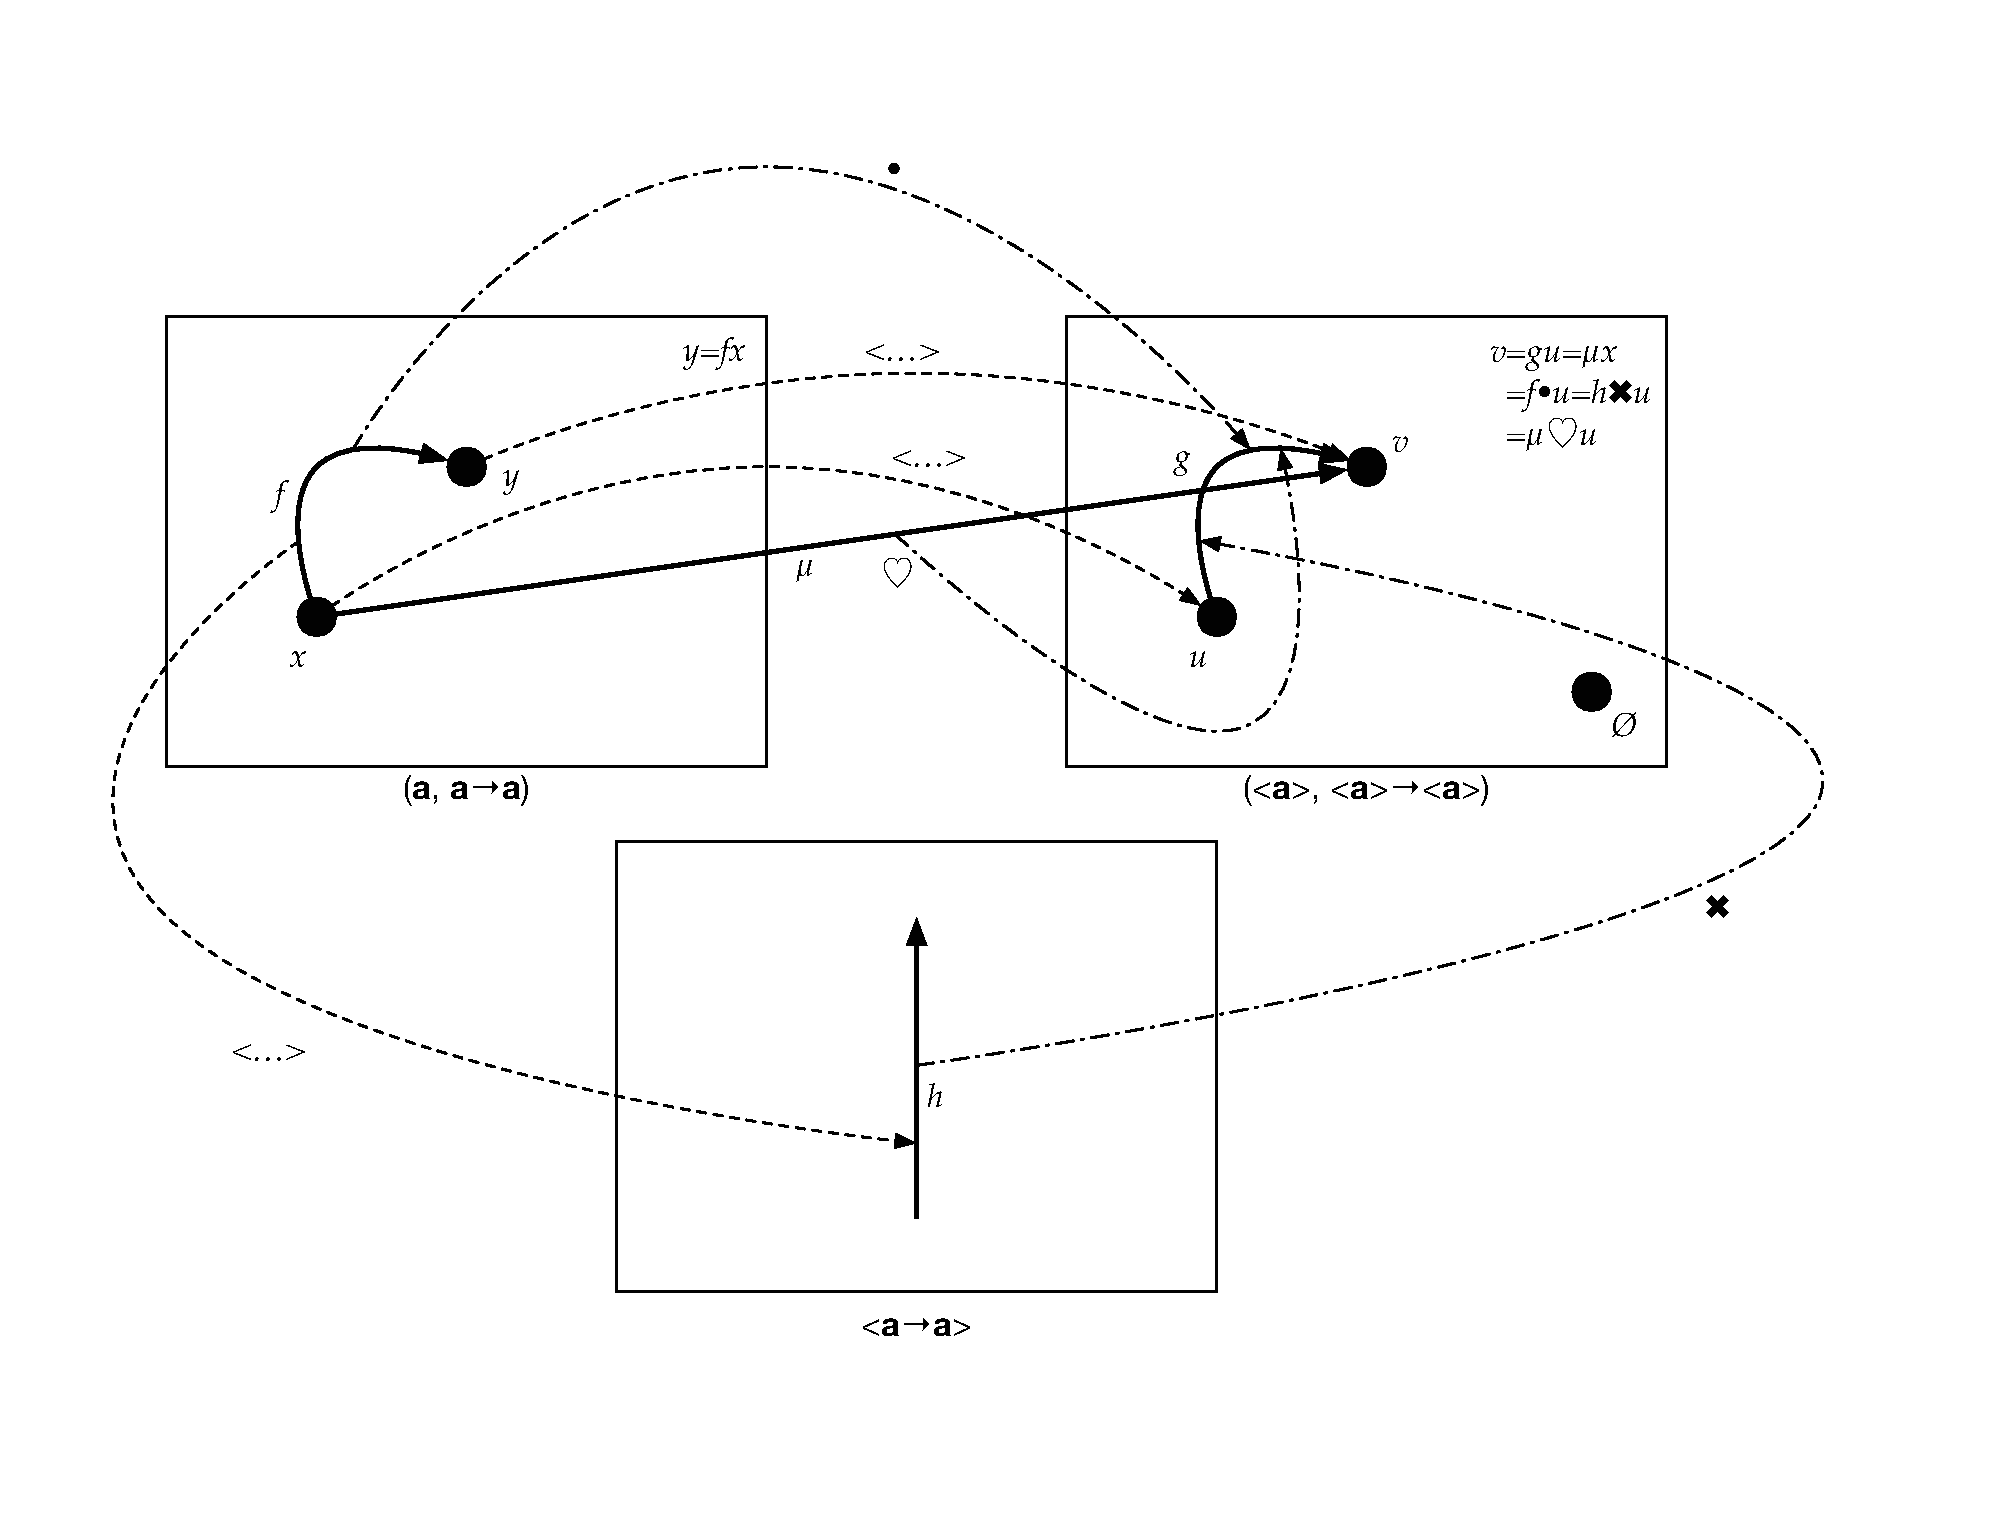
\includegraphics[width=100mm]{fig/functor.eps}
\end{center}
\caption{...}
\label{fig:functor}
\end{figure*}

% \section{IOモナド*}

\begin{table*}
\label{tab:monadplus}
\caption{型と型クラスの関係}
\begin{center}
\begin{tabular}{||c||c|c|c|c|c|c||}
\hline
\multirow{4}{*}{型$\backslash$型クラス}
  &\multicolumn{6}{|c||}{$\mMonadPlusTypeClass$}\\
\cline{2-7}
\multirow{3}{*}{}
  &\multicolumn{4}{|c|}{$\mMonadTypeClass$}
  &\multicolumn{2}{|c||}{$\mMonoidTypeClass$}\\
\cline{3-5}
\multirow{2}{*}{}
  &
  &\multicolumn{3}{|c|}{$\mApplicativeTypeClass$}
  &\multicolumn{2}{|c||}{}\\
\cline{5-5}
\multirow{1}{*}{}
  &
  &\multicolumn{2}{|c|}{}
  &$\mFunctorTypeClass$
  &\multicolumn{2}{|c||}{}\\
\hline\hline
一般コンテナ
  &$\mBind$
  &$\mPureWith{x}$
  &$\mAppMap$
  &$\mMap$
  &
  &\\
\hline
一般モノイド
  &
  &
  &
  &
  &$\mZero$
  &$\mPlus$\\
\hline
リスト
  &$\mBindList$
  &$[x]$
  &$\mAppMapList$
  &$\mMapList$
  &$\mEmptyList$
  &$\mAppend$\\
\hline
Maybe
  &$\mBindMaybe$
  &$\mJustWith{x}$
  &$\mAppMapMaybe$
  &$\mMapMaybe$
  &$\mNothing$
  &($x$ の型に依存)\\
\hline
関数
  &$\mBindFunc$
  &$\mFuncWith{x}$
  &$\mAppMapFunc$
  &$\mMapFunc$
  &$\mAnonParam$
  &$\mComp$\\
\hline
整数
  &
  &
  &
  &
  &$0$
  &$+$\\
\hline
整数
  &
  &
  &
  &
  &$1$
  &$*$\\
\hline
\end{tabular}
\end{center}
\end{table*}

\section{余談:モナドとしての関数}

関数はアプリカティブ関手であった.関数のピュア演算子とアプリカティブマッ
プ演算子はそれぞれ
\begin{align}
\mFuncWith{x}&=\mLambdaEXP{\mAnyParam}{x}\\
g\mAppMapFunc f&=\mLambdaEXP{x}{gx(fx)}
\end{align}
であった.
% 関数ピュア演算子は,任意の引数 $x$ を関数に置き換える.ただし,その関数は引数を捨てて元の変数 $x$ を返す.例えば
% \begin{equation}
% x=\mFuncWith{x}y
% \end{equation}
% と,ダミー変数 $y$ を使って中身の $x$ を取り出せる.

関数のバインド演算子 $\mBindFunc$ を考えておこう.関数のバインド演算子
は
\begin{equation}
g\mBindFunc f=\mLambdaEXP{x}{g(fx)x}
\end{equation}
と定義する.ピュア演算子とバインド演算子から,関数のマップ演算子を
\begin{align}
\mFuncWith{g\mAnonParam}\mBindFunc f
&=\mLambdaEXP{x}{\mFuncWith{g\mAnonParam}(fx)x}\\
&=\mLambdaEXP{x}{\mFuncWith{g(fx)}x}\\
&=\mLambdaEXP{x}{(\mLambdaEXP{\mAnyParam}{g(fx)})x}\\
&=\mLambdaEXP{x}{g(fx)}\\
&=g\mComp f\\
&=g\mMapFunc f
\end{align}
のように合成できる.

まとめると
\begin{align}
\mFuncWith{x}&=\mLambdaEXP{\mAnyParam}{x}\\
g\mMapFunc f&=\mLambdaEXP{x}{g(fx)}=g\mComp f\\
g\mAppMapFunc f&=\mLambdaEXP{x}{gx(fx)}\\
g\mBindFunc f&=\mLambdaEXP{x}{g(fx)x}
\end{align}
である.

% ***Reason***
% http://south37.hatenablog.com/entry/2014/04/27/Haskell%E3%81%AB%E3%81%8A%E3%81%91%E3%82%8B%E3%83%A2%E3%83%8A%E3%83%89
% https://ja.wikipedia.org/wiki/%E3%83%A2%E3%83%8A%E3%83%89_(%E3%83%97%E3%83%AD%E3%82%B0%E3%83%A9%E3%83%9F%E3%83%B3%E3%82%B0)

\separator

関数はモノイドとしての性質も持つ.関数 $\mId=\mAnonParam$ とすると,任
意の関数 $f$ に対して
\begin{equation}
\mId\mComp f=f\mComp\mId=f
\end{equation}
であるから,関数全体の集合を $\mFSet$ で表すと,組み合わせ
$(\mFSet,\mComp,\mId)$ はモノイドである.

モナドでありモノイドである型クラスを\keyword{モナドプラス}と呼ぶ.関数
はモナドプラスである.

今まで出てきた型と型クラスの関係を表\ref{tab:monadplus}に示す.Maybeに
関しては $\mA $ 型がモノイドである場合に限って $\mMaybeType{a}$
型もモノイドである.

\section{この章のまとめ*}

\begin{enumerate}
\item ...
\end{enumerate}


\begin{note}{...}
...
\end{note}

% http://itpro.nikkeibp.co.jp/article/COLUMN/20120110/378061/

\chapter{IO}
\label{ch:io}

A...

\section{アクション}

計算機の状態を変えることを\keyword{副作用}と呼ぶ.副作用とは変数への破
壊的代入に他ならない.例えば,計算機は画面やプリンタに何かを出力するが,
それは画面やプリンタという「変数」を書き換えていることになる.また例え
ば擬似乱数の生成も副作用である.呼び出されるたびに異なる値を返す擬似乱
数生成関数は,そのたびに計算機の内部状態を書き換えているのである.

副作用を持つ関数を\keyword{アクション}と呼ぶ.アクションは値を持つが,
その値は計算の実行時までわからない.例えば擬似乱数を生成するアクション
$\mRand$ があるとしよう.これを変数 $\alpha$ に
\begin{equation}
\alpha=\mRand
\end{equation}
と代入しても,変数 $\alpha$ に擬似乱数が代入されるわけではない.「擬似
  乱数を生成する」というアクションが $\alpha$ に代入されたのだ.

では,いつ「擬似乱数を生成する」アクションが実行されるのだろうか.それ
は,プログラムがまさに計算機の状態を変えるタイミング,つまりプログラム
が実行されるタイミングなのである.そのためには,プログラムそのものをア
クションで表しておかないといけない.我々はプログラム全体を $\omega$ で
表すことにしよう.

プログラムが計算機状態を変える一例として,画面に値を出力することを考え
る.画面に値を出力するアクションを $\mPutStr$ と名付けよう.例えば次の
プログラム例は,画面に ``Hello, world.'' と書き出すものとする.
\begin{equation}
\omega=\mPutStr s\mWhereIsEXP{s}{\mString{``Hello, world.''}}
\end{equation}
アクション $\mPutStr$ は変数を一つとり,その値を画面へ出力すなち破壊的
代入を行う.では $\omega=\mPutStr\alpha$ とすればアクション $\alpha$
が実行されて,晴れて擬似乱数が生成され,その値が画面へ出力されるだろう
か.もちろんそうはならないのである.

ここに $\alpha$ はアクションであり,変数ではない.一方で,アクション
$\mPutStr$ は変数を受け取る.つまり,アクションから何らかの方法で値を
「安全に」抜き取らないといけない.ここで安全性にこだわるのは,アクショ
ン $\alpha$ が副作用を持つからである.副作用を参照透過な変数へ伝播させ
てはいけない.副作用を持つアクションは,副作用を持つアクションへのみ受
け継がれなければならない.

この話は何かと似ていないだろうか.そう,Maybeである.一度ゼロ除算の可
能性に汚染されたコンテナ変数は,コンテナから出すことが許されないのであ
る.Maybeを返す関数$f$の戻り値
\begin{equation}
  \begin{aligned}
    fx&\mGuard{x\neq0}=\mJustWith{1/x}\\
    &\mGuard{\mOtherwise}=\mNothing
  \end{aligned}
\end{equation}
を,別の関数
\begin{equation}
  gy=1+y
\end{equation}
に渡そうと思ったら,
\begin{equation}
  g\mBind fx
\end{equation}
のようにバインド演算子で合成しなければならなかった.

我々はアクションにもバインド演算子を拡張して,
\begin{equation}
  \omega=\mPutStr\mBind\alpha
\end{equation}
とする.これは第\ref{ch:monad}章で見たバインド演算子と同じものである.
同じバインド演算子が使えるカラクリは,次節で見ていくことにする.

\section{IOモナド}

ある関数 $c$ が引数を取らず,いつも決まった $\mDoubleType$ 型の数を返
すとしよう.そうすると,関数 $c$ の型は単純に $\mDoubleType$ である.

呼び出すたびに異なる擬似乱数を返すアクション $\mRand$ もまた毎回
$\mDoubleType$ 型の数を返す.そこで $\mRand$ も $\mDoubleType$ 型とし
たいところだが,こちらは関数ではなくアクションである.そこを区別するた
めに,$\mRand$ の型は $\mIODoubleType$ 型と $\mIOType{\dotsb}$ に入れ
て区別する.\footnote{\haskell では $\mIODoubleType$ のことを \code{IO
Double} と書く.}

呼び出しても何も返さないアクションはどのような型を持つべきだろう.何も
返さない関数というものは無意味だが,アクションは副作用を持つので,何も
返さないものがあっても良いのである.何も返さないことを「空っぽ」を返す
と読み替えて,何も返さないアクションの型を $\mIOUnitType$ 型としよう.
ここに $\mUnitType$ は「空っぽ」の意味で,ユニット型と読む.
$\mIOUnitType$ 型のアクションの例は,画面に値を出力する $\mPutStr$ ア
クションである.\footnote{\haskell では $\mIOUnitType$ のことを
  \code{IO ()} と書く.}

キーボードからの入力を受け取るアクションもある.そのアクションを
$\mReadLn$ としよう.アクション $\mReadLn$ は文字列型を返すので,その
型は $\mIOStringType$ である.\footnote{\haskell では $\mIOStringType$
のことを \code{IO String} と書く.}

アクション $\mPutStr,\mReadLn,\mRand$ は計算機の状態を変化させる.アク
ション $\mPutStr,\mReadLn$ はOSのシステムコールを発行して,前者ならビ
デオメモリの値を書き換えるし,後者ならシリアルインタフェースの入力バッ
ファをフラッシュする.アクション $\mRand$ は呼ばれるたびに内部のカウン
タ値を一つ進める.これらのアクションは参照透過性を破壊する.そのために,
プログラムの他の部分から隔離されねばならない.その隔離のメカニズムを提
供するのがモナドである.

$[\mA]$ 型が $\mA $ 型のリストであるように,$\mIOType{a}$
型は $\mA $ 型の\keyword{IO}である.そしてリストがモナドであるよ
うに,IOもまたモナドである.モナドには,バインド演算子と,アプリカティ
ブ関手から引き継いだピュア演算子の二つが必要であった.アプリカティブ関
手から引き継いだアプリカティブマップ演算子はバインド演算子とピュア演算
子の二つから合成できるし,関手から引き継いだマップ演算子もまたアプリカ
ティブマップ演算子とピュア演算子から合成できるから,アプリカティブマッ
プ演算子とマップ演算子は改めて実装しておく必要はない.

$\mIOUnitType$ 型の場合,ピュア演算子は何も返す必要がないから
\begin{equation}
\mPureWith{\mAnyParam}=()
\end{equation}
であるとする.

% ここに $\mTupleWith{}$ は空のタプルで,「ユニット」と呼ぶ.一方で
% $\mIOUnitType$ 型のバインド演算子は,処理系の奥深くに隠されている.

% 実装依存である.


% http://tnomura9.exblog.jp/12069145/

\section{do記法}

モナドを使った書き方が従来のプログラムの記法からあまりにもかけ離れてい
ることに,\haskell の設計者は気づいていたようで,\haskell には次に述べ
る\keyword{do記法}という記法が用意されている.このdo記法はもちろんシン
タックスシュガーで,新しいことは何もない.

例えば $\omega=\mPutStr\mBind\alpha\mWhereIsEXP{\alpha}{\mRand}$ をdo記法
を用いて書き直すと
\begin{equation}
\label{eq:do-print-random}
\omega=\mDo{a\mDoEq\mRand\mDoNext\mPutStr a}
\end{equation}
となる.ここで変数 $a$ は $\{\dotsb\}$ の中でだけ参照できる変数である.バインド演算子が副作用やゼロ除算汚染を中に閉じ込めたように,do記法の括弧は副作用や汚染を閉じ込める役割を果たす.\footnote{\haskell では \code{omega = do \{ a <- rand; putStr
a \}} と書くか,または $\mDoNext$ を改行に置き換えて
\begin{verbatim}
  omega = do
    a <- rand
    putStr a
\end{verbatim}
と書く.}

ここで,同様なことをする\python プログラムを見てみよう.
\begin{pythoncode}
\begin{verbatim}
import random
define main:
  a = random.random() # (1)
  print(a)            # (2)
\end{verbatim}
\end{pythoncode}
コード中の \code{(1)} の行で $a\mDoEq\mRand$ を実行し,\code{(2)} の行
で $\mPutStr a$ を実行していると思えば,このコードと式
\eqref{eq:do-print-random}の順序はそっくり同じである.もちろんこのdo記
法はバインド演算子を使った式を切り貼りして,順序を入れ替えただけである.

do記法には $\mDoEq$ の他に,我々の $\mLetKeyword$ とよく似た
$\mDoLetKeyword$ という構文が用意されている.この $\mDoLetKeyword$ は
局所変数の導入に用いられて,例えば
\begin{equation}
\omega=\mDo{\mDoLet{y}{fx}\mDoNext\alpha y}
\end{equation}
のように使う.

以下に,do記法を使った例を示す.
\begin{gather}
\mDo{\alpha x}=\alpha x\\
\mDo{y\mDoEq\alpha x\mDoNext\beta y}=\beta\mBind\alpha x\\
\mDo{\alpha x\mDoNext\beta y}=(\mLambdaEXP{\mAnyParam}{\beta y})\mBind \alpha x\label{eq:do-alpha-beta}\\
\mDo{\mDoLet{y}{fx}\mDoNext\alpha y}=\alpha y\mWhereIsEXP{y}{fx}\\
\mDo{y\mDoEq\alpha x\mDoNext\mDoLet{z}{fy}\mDoNext\beta z}
=\beta\mBind{}(f\mMap\alpha x)
\end{gather}
より複雑な例も挙げる.
\begin{multline}
\mDo{y\mDoEq\alpha x\mDoNext y'\mDoEq\alpha'x'\mDoNext\mDoLet{z}{fyy'}
\mDoNext\beta z}\\
=\beta\mBind{}(f\mMap\alpha x\mAppMap\alpha'x')
\end{multline}
最後にdo記法中に変数を2回以上使いまわす例を示す.
\begin{multline}
\mDo{y\mDoEq\alpha x\mDoNext y'\mDoEq\alpha'x'\mDoNext\mDoLet{z}{fyy'}\mDoNext\beta z\mDoNext\mDoLet{z'}{f'yy'}\mDoNext\beta'z'}\\
=(\mLambda yy'\mLambdaArrow{}((\mLambdaEXP{\mAnyParam}{\mLetInEXP{z}{fyy'}{\beta z}})\\
\mBind{}(\mLetInEXP{z'}{f'yy'}{\beta'z'}))) (\alpha x)(\alpha'x')
\end{multline}
この例では変数 $y,y'$ が2回使われている.

% なお $\mFuncWith{f}=\mLambdaEXP{\mAnyParam}{f}$ の関係を用いると式\eqref{eq:do-alpha-beta}はより簡潔に
% \begin{equation}
% \mDo{\alpha x\mDoNext\beta y}=\mFuncWith{\beta y}\mBind\alpha x
% \end{equation}
% と書ける.

我々はバインド演算子を使った通常の記法とdo記法のいずれか読みやすい方を採用すれば良い.

% main =
% do
%   r <- rand
%   print r

% http://qiita.com/saltheads/items/6025f69ba10267bbe3ee

\separator

バインド演算子には,左右の引数を入れ替えた\keyword{右バインド演算子}が
ある.右バインド演算子は $\mBindRight$ と書き,
\begin{equation}
\alpha x\mBindRight\beta=\beta\mBind\alpha x
\end{equation}
であるとする.\footnote{\haskell では $\alpha x\mBindRight\beta$ を \code{alpha x >>= beta} と書く.}

\section{余談:関数であるということ*}

IOモナドの変数は,たとえ値を読み出すだけであっても必ず関数適用が必要で
ある.それは,IOモナドの変数が「自分が読み出されたこと」を知る必要があ
るからである.IOモナドの変数は,自分が読み出されたタイミングで副作用を
発生させる.これは\objectivec や\swift に見られる getter メソッドと同
じ考え方である.

IOモナドの変数値を読み出すために行われる関数呼び出しはダミーである場合
があり,戻り値はしばしば捨てられる.

変数をダミーの関数で包み,それをさらにIOモナドで包んだのがIOモナド変数
である.

もうひとつ,アクションが関数でなければならない理由がある.\haskell は
いつも遅延評価を行うことを思い出してもらいたい.\python であれば,式は
書かれた順に評価される.しかし,例えば
\begin{align}
y_1&=f_1x_1\\
y_2&=f_2x_2
\end{align}
という式があった場合,関数 $f_1$ と $f_2$ のどちらが先に評価されるか,
あるいは同時に評価されるかは\haskell では未定義である.\haskell で唯一
計算順序が保証されているのは,関数適用である.例えば
\begin{equation}
y=g_2(g_1x)
\end{equation}
であれば,確実に関数 $g_1$ が関数 $g_2$ よりも先に評価される.

直列に評価したい関数の戻り値が,いつも次の関数の引数の型と一致している
とは限らないし,次の関数(アクション)が引数を取らない可能性もある.も
し関数 $g_2$ が引数を取らなければ
\begin{equation}
\mFuncWith{g_2}(g_1x)
\end{equation}
とする.この時,関数適用 $(g_1x)$ の結果は単純に捨てられる.
\footnote{\clang では \code{void} 型を返す関数 \code{void g1(int)} を引
  数を取らない関数 \code{int g2(void)} に「食わせる」ことが可能で,
  \code{g2(g1(x))} は正しいコードである.もっとも\clang プログラマは
  \code{g1(x), g2()} という書き方の方を好むであろう.}

\separator

ふたつのアクション $\alpha_1,\alpha_2$ があり,アクション $\alpha_2$
が引数を取らない場合,その二つを合成するには
\begin{equation}
\label{eq:ignore-return}
\alpha_1 x\mBindRight\mFuncWith{\alpha_2}
\end{equation}
とする.式\eqref{eq:ignore-return}はしばしば
% \begin{equation}
% g_2\twoheadleftarrow g_1x=\mFuncWith{g_2}(g_1x)
% \end{equation}
% または
\begin{equation}
\alpha_1 x\mBindRightIgnore\alpha_2=\alpha_1x\mBindRight\mFuncWith{\alpha_2}
\end{equation}
なる演算子 $\mBindRightIgnore$ を用いて記述される.\footnote{\haskell
  では $\alpha_1x\mBindRightIgnore\alpha_2$ を \code{alpha1 x >>
    alpha2} と書く.}

\section{この章のまとめ*}

\begin{enumerate}
\item do記法.
\end{enumerate}

\begin{note}{...}
...
\end{note}


\chapter{データ型の定義*}

...

\section{データ型}

我々はしばしば新しい集合を考える必要に迫られる.例えば,イチ,ニ,サン,
タクサンからなる集合
\begin{equation}
\mSet{Num}\mDefEq\{\mNumOne,\mNumTwo,\mNumThree,\mNumMany\}
\end{equation}
を考えることがあるだろう.集合 $\mSet{Num}$ の元 $n\mIn\mSet{Num}$ は
$\mNumOne$, $\mNumTwo$, $\mNumThree$, $\mNumMany$ のいずれかの値を取る
ことになる.

数学者は新しい集合を定義するが,\haskell プログラマは新しいデータ型を定
義する.集合 $\mSet{Num}$ の定義の代わりに,我々はデータ型
$\mType{Num}$ を
\begin{equation}
  \mDataType\;\mType{Num}
  =\mNumOne\mValueOr\mNumTwo\mValueOr\mNumThree\mValueOr\mNumMany
\end{equation}
のように書いて定義するものとする.式の先頭にある $\mDataType$ は,この
式がデータ型の定義であることを示すタグである.部分的にアンダーラインが
引かれているのは,\haskell が $\mDataType$ を \code{data} と省略してし
まうからである.これは不本意なことだが,文字数節約のために仕方ない.こ
こに $\mSet{Num}$ は型コンストラクタ,$\mNumOne$, $\mNumTwo$,
$\mNumThree$, $\mNumMany$ は値コンストラクタである.
\footnote{\haskell では \code{data Num = One | Two | Three | Many} と書
  く.}

% 値コンストラクタを列挙したデータ型を\keyword{代数型}と呼ぶ.

この節で紹介したデータ型の定義は\clang で言う \code{enum} に近い.他に
\clang で言う \code{struct} や \code{union} すなわち構造体や共用体もこ
の $\mDataType$ 文で定義できるが,これは次節で見ることにする.

\separator

新しいデータ型がある型クラスに属すとき,$\mDataType$ 文でそれを同時に
宣言できる.例えば $\mType{Num}$ 型は同値演算子 $(\equiv)$ を持つこと
が自然である.型 $\mType{Num}$ が $\mEqTypeClass$ 型クラスに属すとき,
\begin{equation}
  \mDataType\;
  \mType{Num}
  =\mNumOne\mValueOr\mNumTwo\mValueOr\mNumThree\mValueOr\mNumMany
  \mDeriving\mEqTypeClass
\end{equation}
のように書く.\footnote{\haskell では \code{data Num = One | Two |
Three | Many deriving Eq} と書く.}

型 $\mType{Num}$ の同値演算子 $(\equiv)$ の実装は
\ref{sec:type-class-and-instance}節で見ることにする.

\section{レコード構文}

データ型の定義では,値コンストラクタにパラメタを与えることもできる.例
えば $\mType{Rectangle}$ という型を考えよう.この型は,始点の平面座標
と幅,高さで合計4個の $\mFloatType$ のパラメタを取るものとする.このと
き
\begin{multline}
  \label{eq:rectangle}
  \mDataType\;
  \mType{Rectangle}\\
  =\mValueWith{Rectangle}
  {\mFloatType\,\mFloatType\,\mFloatType\,\mFloatType}
  \mDeriving\mEqTypeClass
\end{multline}
という風にデータ型の定義を行う.\footnote{\haskell では \code{data
Rectangle = Rectangle Float Float Float Float} と書く.}

$\mType{Rencatngle}$ 型の変数は次のように初期化する.
\begin{equation}
  \left\mBrace
  \begin{aligned}
    r&\mIn\mType{Rectangle}\\
    r&=\mValueWith{Rectangle}{1\,2\,3\,4}
  \end{aligned}
  \right.
\end{equation}
これは\clang で言う \code{struct} と似た用法である.\footnote{\haskell
では
\begin{verbatim}
  r :: Rectangle
  r = Rectangle 1 2 3 4
\end{verbatim}
と書く.}

$\mType{Rectangle}$ 型から中身を取り出すには,次のような関数を用意して
おかねばならない.
\begin{align}
  x\mValueWith{Rectangle}{x\,\mAnyParam\,\mAnyParam\,\mAnyParam}
  &=x\\
  y\mValueWith{Rectangle}{\mAnyParam\,y\,\mAnyParam\,\mAnyParam}
  &=y\\
  width\mValueWith{Rectangle}{\mAnyParam\,\mAnyParam\,w\,\mAnyParam}
  &=w\\
  height\mValueWith{Rectangle}{\mAnyParam\,\mAnyParam\,\mAnyParam\,h}
  &=h
\end{align}
この面倒は,次のシンタックスシュガーを使うことで軽減される.
\footnote{\haskell では
\begin{verbatim}
  x      Rectangle x _ _ _ = x
  y      Rectangle _ y _ _ = y
  width  Rectangle _ _ w _ = w
  height Rectangle _ _ _ h = h
\end{verbatim}
と書く.}

型 $\mType{Rectangle}$ のようにパラメタが多いときは,パラメタに名前が
あると便利である.そこで利用できるのが\keyword{レコード構文}である.レ
コード構文を使うと,式\eqref{eq:rectangle}は
\begin{multline}
  \mDataType\;\mType{Rectangle}\\
  =\mValueRecordBeginWith{Rectangle}
  x\mIn\mFloatType,
  y\mIn\mFloatType,
  width\mIn\mFloatType,
  height\mIn\mFloatType
  \mValueRecordEnd\\
  \mDeriving\mEqTypeClass
\end{multline}
のように書き直すことができる.\footnote{\haskell では
\begin{verbatim}
  data Rectangle = Rectangle {
      x      :: Float,
      y      :: Float,
      width  :: Float,
      height :: Float
    }
    deriving Eq
\end{verbatim}
と書く.}

レコード構文を用いると,型から中身を取り出す関数は自動的に定義される.
また
\begin{equation}
  r=
  \mValueRecordWith{Rectangle}{
    x=1,
    y=2,
    width=3,
    height=4
  }
\end{equation}
のようなレコード構文専用の初期化を行っても良いし,従来の初期化方法を用
いても良い.\footnote{\haskell では\code{r = Rectangle \{ x = 1, y =
    2, width = 3, height = 4 \}} と書く.}

\separator

データ型の定義には,複数の値コンストラクタを指定できる.そのため
\begin{multline}
\mDataType\;\mType{Shape}
=\mValueWith{Circle}{\mFloatType\,\mFloatType}\\
\mValueOr
\mValueWith{Triangle}{\mFloatType\,\mFloatType\,\mFloatType}
\end{multline}
のようなデータ型の定義も可能である.この例では型 $\mType{Shape}$ は値
コンストラクタ $\mValueConstructor{Circle}$ または
$\mValueConstructor{Triangle}$ によって初期化され,それぞれ2個
または3個の $\mFloatType$ 型のパラメタを取る.\footnote{\haskell では
\code{data Shape = Circle Float Float | Triangle Float Float Float}
と書く.}

\section{型クラスとインスタンス化}
\label{sec:type-class-and-instance}

型クラスとは,複数の型が持つ共通のインタフェースである.その複数の型を
いま $\mA $ で表すこととして,型 $\mA $ が型クラス
$\mEqTypeClass$ に属すとしよう.型クラス $\mEqTypeClass$ は等号
$(\equiv)$ と不等号 $(\neq)$ をインタフェースとして持つ.このことを
\begin{equation}
  \mTypeClassDecl\mathop{\mEqTypeClass}\mSuperSet\mA\mWhere{}
  \left\{
  \begin{aligned}
    &(\equiv)\mIn\mProjEXP{\mA }{\mProjEXP{\mA }{\mBoolType}}\\
    &(\neq)\mIn\mProjEXP{\mA }{\mProjEXP{\mA }{\mBoolType}}\\
    &x\equiv y=\neg(x\neq y)\\
    &x\neq y=\neg(x\equiv y)
  \end{aligned}
  \right.
\end{equation}
と書く.\footnote{\haskell では$\mTypeClassDecl$ を \code{class} と書く.ま
  た $\mSuperSet$ を省略して,
\begin{verbatim}
  class Eq a where
    (==) :: a -> a -> Bool
    (/=) :: a -> a -> Bool
    x==y = not(x/=y)
    x/=y = not(x==y)
\end{verbatim}
と書く.}

ここで宣言したのは等号,不等号というインタフェースが「ある」という事だ
けで,その実装は未定義である.等号,不等号の実装は次に述べる
$\mInstance$ 文を使う.

型クラス $\mEqTypeClass$ に属す型 $\mA $ は等号と不等号を持つ.我々
の型 $\mType{Num}$ が型クラス $\mEqTypeClass$ に属すことを宣言し,型ク
ラス $\mEqTypeClass$ が備えるべき等号,不等号を実装するには
\begin{equation}
  \mInstance\;\mEqTypeClass\mSuperSet\mType{Num}
  \mWhere{}
  \left\{
  \begin{aligned}
    \mNumOne\equiv\mNumOne&=\mTrue\\
    \mNumTwo\equiv\mNumTwo&=\mTrue\\
    \mNumThree\equiv\mNumThree&=\mTrue\\
    \mNumMany\equiv\mNumMany&=\mTrue\\
    \mAnyParam\equiv\mAnyParam&=\mFalse
  \end{aligned}
  \right.
\end{equation}
とする.これを\keyword{型クラスのインスタンス化}と呼ぶ.
\footnote{\haskell では
\begin{verbatim}
  instance Eq Num where
    One==One     = True
    Two==Two     = True
    Three==Three = True
    Many==Many   = True
    _==_         = False
\end{verbatim}
と書く.}

型クラスは\keyword{継承関係}を持てる.型クラス $\mOrdTypeClass$ は型ク
ラス $\mEqTypeClass$ から等号,不等号を継承し「小なりイコール」
$(\le)$ を追加する.
\begin{equation}
  \mTypeClassDecl\;\mEqTypeClass\mSuperSet\mA 
  \mSuperClass\mathop{\mOrdTypeClass}\mA 
  \mWhere{}(\le)\mIn\mProjEXP{\mA }{\mProjEXP{\mA }{\mBoolType}}
\end{equation}
型クラス $\mOrdTypeClass$ に属する型は,等号,不等号,小なりイコールと,
それらから派生させることのできる大なり $(>)$,大なりイコール $(\ge)$,
小なり $(<)$,および最大値をとる関数 $\max$ と最小値をとる関数 $\min$
を持つ.\footnote{\haskell では
\begin{verbatim}
  class (Eq a) => Ord a where (<=) :: a -> a -> Bool
\end{verbatim}
と書く.}

\separator

型は複数の型クラスに同時に属すことができる.例えば型 $\mType{Num}$ は
型クラス $\mEqTypeClass$ と同時に型クラス $\mOrdTypeClass$ に属すこと
もできる.それには
\begin{equation}
\mDataType\;\mType{Num}
=\mNumOne\mValueOr\mNumTwo\mValueOr\mNumThree\mValueOr\mNumMany
\mDeriving{}(\mEqTypeClass,\mOrdTypeClass)
\end{equation}
とする.\footnote{\haskell では
\begin{verbatim}
  data Num = One | Two | Three | Many deriving (Eq, Ord)
\end{verbatim}
と書く.}

型クラス $\mOrdTypeClass$ のインスタンスは小なりイコール演算子 $(\le)$
が定義されていなければならない.我々は
\begin{equation}
  \mInstance\;\mOrdTypeClass\mSuperSet\mType{Num}
  \mWhere{}
  \left\{
  \begin{aligned}
    \mNumOne\le\mNumOne&=\mTrue\\
    \mNumOne\le\mNumTwo&=\mTrue\\
    \mNumOne\le\mNumThree&=\mTrue\\
    \mNumOne\le\mNumMany&=\mTrue\\
    \mNumTwo\le\mNumTwo&=\mTrue\\
    \mNumTwo\le\mNumThree&=\mTrue\\
    \mNumTwo\le\mNumMany&=\mTrue\\
    \mNumThree\le\mNumThree&=\mTrue\\
    \mNumThree\le\mNumMany&=\mTrue\\
    \mNumMany\le\mNumMany&=\mTrue\\
    \mAnyParam\equiv\mAnyParam&=\mFalse
  \end{aligned}
  \right.
\end{equation}
のように $\mType{Num}$ の $\le$ 演算子を定義することができる.

\section{余談:型シノニム}

データ型には\keyword{シノニム}(別名)がつけられる.例えば
$\mCharType$ のリスト $[\mCharType]$ は
\begin{equation}
  \mTypeSynonym\;
  \mStringType
  =[\mCharType]
\end{equation}
とすることで,別名 $\mStringType$ を与えることができる.\haskell では
$\mTypeSynonym$ を \code{type} と省略してしまう.これは残念なことだが,
\clang の \code{typedef} のようなものだと思って割り切るしかない.
\footnote{\haskell では \code{type String = [Char]} と書く.}

\section{この章のまとめ*}

\begin{enumerate}
\item ...
\end{enumerate}

\begin{note}{メタクラス}
オブジェクト指向言語の多くが「クラス」と呼ぶものを,\haskell は「型」と呼ぶ.

% クラスのクラスをメタクラスと言う.

% メタクラスのクラスはメタメタクラスである.全てのメタクラスはメタメタクラスに属す.それ故,メタメタクラスもまたメタメタクラスに属す.
\end{note}


\chapter{多相型の定義}
\label{ch:parametric-data-type}
...

\section{多相型}

Maybeのように型パラメタを取る型を\keyword{多相型}と呼ぶ.多相型はどの
ように定義されるかと言うと,
\begin{equation}
\mDataTypePolymorphic\;\mMaybeTypeConstructor\,\mA 
=\mJustWith{\mA }\mValueOr\mNothing
\end{equation}
のように,やはり $\mDataType$ を使って定義される.念のため型パラメタを
取る場合は $\mDataTypePolymorphic$ と区別しておこう.\footnote{\haskell
は $\mDataType$ と $\mDataTypePolymorphic$ を区別せず,
$\mDataTypePolymorphic\;\mMaybeTypeConstructor\mA 
=\mJustWith{\mA }\mValueOr\mNothing$ を \code{data Maybe a =
Just a | Nothing} と書く.}
% この $\mJustWith{\mA }$ は $\mA $ のMaybe型 $(\mMaybeType{a})$ という意味ではなく,$\mA $ 型の変数を型コンストラクタ $\mJustWith{\dotsb}$ に入れなさいという意味.

Maybeが型クラス $\mEqTypeClass$ に属すものとして,$\mEqTypeClass$ から
のインスタンス化をしておこう.ここでも型パラメタ付きの $\mInstance$ を
仮に $\mInstancePolymorphic$ とすると次のように書けそうである.
\begin{multline}
\mInstancePolymorphic\;
\mEqTypeClass\mSuperSet{}(\mMaybeTypeConstructor\,\mA )\\
\mWhere
\left\{
\begin{aligned}
\mJustWith{x}\equiv\mJustWith{y}&=x\equiv y\\
\mNothing\equiv\mNothing&=\mTrue\\
\mAnyParam\equiv\mAnyParam&=\mFalse
\end{aligned}
\right.
\end{multline}
残念ながら,この式は $\mA $ 型の変数 $x,y$ の間に等号 $(\equiv)$
が定義されていることが隠れた前提になっているため,正しくない.我々は
$\mA $ が型クラス $\mEqTypeClass$ に属すことを要求するので,次の
ように言い換える.
\begin{multline}
\mInstancePolymorphic\;
\mEqTypeClass\mSuperSet\mA 
\mSuperClass
\mEqTypeClass\mSuperSet{}(\mMaybeTypeConstructor\,\mA )\\
\mWhere
\left\{
\begin{aligned}
\mJustWith{x}\equiv\mJustWith{y}&=x\equiv y\\
\mNothing\equiv\mNothing&=\mTrue\\
\mAnyParam\equiv\mAnyParam&=\mFalse
\end{aligned}
\right.
\end{multline}
この $\mEqTypeClass\mSuperSet\mA \mSuperClass$ の部分が「以下
$\mA $ 型は $\mEqTypeClass$ 型クラスに属すものとして」という意
味になる.\footnote{\haskell では
\begin{verbatim}
  instance Eq a => Eq (Maybe a) where
    Just x == Just y = x==y
    Nothing==Nothing = True
    _==_             = False
\end{verbatim}
と書く.
}

Maybeの間に新たに定義された等号 $(\equiv)$ は次の型を持つ.
\begin{equation}
(\equiv)
\mIn{}\mEqTypeClass\mSuperSet\mA 
\mSuperClass\mProjEXP{\mMaybeType{a}}{\mProjEXP{\mMaybeType{a}}{\mBoolType}}
\end{equation}

\separator

多相型を定義するとき,型パラメタは2個以上与えられても良い.例えば
Eitherは次のように定義できる.
\begin{equation}
\mDataTypePolymorphic\;\mEitherTypeConstructor\,\mA \,\mB 
=\mLeftWith{\mA }
\mValueOr
\mRightWith{\mB }
\end{equation}

\section{自己参照型}

型の定義中に自分自身を参照する型を\keyword{自己参照型}または
\keyword{再帰型}と呼ぶ.例えばリストは
\begin{equation}
\mDataTypePolymorphic\;\mListTypeConstructor\,\mA =\mEmptyList\mValueOr\mA :\mListTypeConstructor\,\mA 
\end{equation}
のように定義できる.

\section{関手の拡張}

型クラス $\mFunctorTypeClass$ はマップ演算子 $(\mMap)$ を提供する.リ
スト型は $\mFunctorTypeClass$ 型クラスのインスタンスなので,
\begin{align}
  \mTypeClassDeclPolymorphic\;
  &\mFunctorTypeClass\mSuperSet\mListTypeConstructor{}
  \mWhere{}
  \mMap\mIn{}\mProjEXP{(\mProjEXP{\mA }{\mB })}
           {\mProjEXP{[\mA]}{[\mB]}}\\
           \mInstancePolymorphic\;
           &\mFunctorTypeClass\mSuperSet\mListTypeConstructor{}
           \mWhere{}\mMap=\mMapList
\end{align}
と定義する.\footnote{\haskell では
\begin{verbatim}
  class    Functor [] where fmap :: (a -> b) -> [a] -> [b]
  instance Functor [] where fmap = map
\end{verbatim}
と書く.}

Maybe型の場合は
\begin{align}
  \mTypeClassDeclPolymorphic\;
  &\mFunctorTypeClass\mSuperSet\mMaybeTypeConstructor\nonumber\\
&\quad\mWhere{}\mMap\mIn{}\mProjEXP{(\mProjEXP{\mA }{\mB })}{\mProjEXP{\mMaybeType{a}}{\mMaybeType{b}}}\\
  \mInstancePolymorphic\;
  &\mFunctorTypeClass\mSuperSet\mMaybeTypeConstructor\nonumber\\
  &\quad\mWhere
  \left\{
  \begin{aligned}
    f\mMap\mJustWith{x}&=\mJustWith{fx}\\
    f\mMap\mNothing&=\mNothing
  \end{aligned}
  \right.
\end{align}
となる.\footnote{\haskell では
\begin{verbatim}
  class Functor Maybe where
    fmap :: (a -> b) -> Maybe a -> Maybe b
  instance Functor Maybe where
    fmap f (Maybe x) = Maybe (f x)
    fmap f Nothing = Nothing
\end{verbatim}
と書く.}

Either型の場合は
\begin{align}
  \mTypeClassDeclPolymorphic\;
&\mFunctorTypeClass\mSuperSet{}(\mathop{\mEitherTypeConstructor}\,\mA )\nonumber\\
&\quad\mWhere{}\mMap\mIn{}\mProjEXP{(\mProjEXP{\mA }{\mB })}{\mProjEXP{\mEitherType{a}{a}}{\mEitherType{a}{b}}}\\
  \mInstancePolymorphic\;
&\mFunctorTypeClass\mSuperSet{}(\mathop{\mEitherTypeConstructor}\,\mA )\nonumber\\
  &\quad\mWhere{}
  \left\{
  \begin{aligned}
    f\mMap{}\mRightWith{x}&=\mRightWith{fx}\\
    f\mMap{}\mLeftWith{x}&=\mLeftWith{x}
  \end{aligned}
  \right.
\end{align}
となる.\footnote{\haskell では
\begin{verbatim}
  class Functor (Either a) where
    fmap :: (a -> b) -> Either a a -> Either a b
  instance Functor (Either a) where
    fmap f (Right x) = Right (f x)
    fmap f (Left x)  = Left x
\end{verbatim}
と書く.}

型に関して一般化すると
\begin{multline}
  \label{eq:fn}
  \mTypeClassDeclPolymorphic\;
  \mFunctorTypeClass\mSuperSet\mTypeConstructor{f}\\
  \mWhere{}
  \mMap
  \mIn{}(\mA\mMapsTo\mB)
  \mMapsTo\mTypeAssemble{f}{a}
  \mMapsTo\mTypeAssemble{f}{b}
\end{multline}
のように書ける.ここで,型 $\mTypeAssemble{f}{a}$ は型
$\mA$ と型コンストラクタ $\mPolymorphicTypeParameter{f}$ から
\begin{equation}
  \mTypeAssemble{f}{a}
  =\mathop{\mTypeConstructor{f}}\mA
\end{equation}
のように作られる.\footnote{\haskell では
  $\mTypeAssemble{f}{a}$ も
  $\mathop{\mTypeConstructor{f}}\mA $ も同様に \code{f a} と書く.
  そこで式\eqref{eq:fn}は
\begin{verbatim}
  class functor f where fmap :: (a -> b) -> f a -> f b
\end{verbatim}
と書く.}

\section{余談: \code{newtype}*}

リストに新しいマップ演算子 $\mZip$ を定義したいとしよう.この演算子
$\mZip$ は
\begin{equation}
  [f,g,h]\mZip\mListWith{x,y,z}
  =[fx,gy,hz]
\end{equation}
のように働くとする.新しいマップ演算子 $\mZip$ のことを我々は
\keyword{ジップ演算子}と呼ぶことにする.

ジップ演算子を定義するにはどうしたら良いだろうか.汎用性を考えると,ジッ
プ演算子もまたリストのアプリカティブマップ演算子であって欲しい.ところ
が,リストには既に $\mAppMapList$ というアプリカティブマップ演算子が定
義されている.念のためにアプリカティブマップ演算子を用いると
\begin{equation}
  [f,g,h]\mAppMapList[x,y,z]
  =[fx,fy,fz,gx,gy,gz,hx,hy,hz]
\end{equation}
である.ある型のインスタンス化は一種類しか行えないので,リスト型に新し
いアプリカティブマップ演算子を追加することは出来ない.

そこで $\mDataTypePolymorphic$ を使ってリスト型をラップした新しい型を作
る.例えば新しい型を $\mZipListType{a}$ とすると
\begin{equation}
  \label{eq:data-type-ziplist}
  \mDataTypePolymorphic\;
  \mathop{\mZipListTypeConstructor}\mA 
  =\mValueRecordWith{ZipList}{\mGetList\mIn{}[\mA]}
\end{equation}
のように定義することになる.念のため,左辺の
$\mZipListTypeConstructor$ は型コンストラクタ,右辺の
$\mValueConstructor{ZipList}$ は値コンストラクタである.すな
わち
\begin{equation}
  \mZipListType{a}
  =\mZipListTypeConstructor\mA 
\end{equation}
である.

こうしておいて,あとは
\begin{multline}
  \mInstancePolymorphic\;
  \mApplicativeTypeClass\mSuperSet\mZipListTypeConstructor\mA\\
  \mWhere
  \left\{
  \begin{aligned}
    \mPureWith{x}
    &=\mZipListWith{\mRepeat x}\\
    \mZipListWith{\mList{f}}\mAppMap\mZipListWith{\mList{x}}
    &=\mZipListWith{\mList{f}\mZip\mList{x}}
  \end{aligned}
  \right.
\end{multline}
と定義する.ここで
\begin{equation}
  \label{eq:zip}
  \left\{
  \begin{aligned}
    (\mZip)\mAnyParam\mEmptyList&=\mEmptyList\\
    (\mZip)\mEmptyList\mAnyParam&=\mEmptyList\\
    (\mZip)(x:\mList{x})(y:\mList{y})&=(x\mApply y):\mList{x}\mZip\mList{y}
  \end{aligned}
  \right.
\end{equation}
であると定義する.

関数 $\mRepeat$ は引数を無限回繰り返すリストを返す関数である.念のため
関数 $\mRepeat$ の実装方法を書いておくと
\begin{equation}
  \left\mBrace
  \begin{aligned}
    &\mRepeat\mIn{}\mProjEXP{[\mA]}{[\mA]}\\
    &\mRepeat x=x:\mRepeat x
  \end{aligned}
  \right.
\end{equation}
である.

任意のリスト $\mList{x}$ と任意の関数リスト $\mList{f}$ ただし
\begin{align}
\mList{x}&=[x_0,x_1,\dotsb]\\
\mList{f}&=[f_0,f_1,\dotsb]
\end{align}
の両方をそれぞれ値コンストラクタで包んでアプリカティブマップ演算子を適
用すると
\begin{equation}
  \mZipListWith{\mList{f}}\mAppMap\mZipListWith{\mList{x}}
  =[f_0x_0,f_1x_1,\dotsb]
\end{equation}
のようにジップ演算子を適用できる.

このままでも問題はないのだが,式\eqref{eq:data-type-ziplist}を次のよう
に書き換えることがより好ましい.
\begin{equation}
  \mNewDataTypePolymorphic\;
  \mZipListTypeConstructor\mA
  =\mZipListRecordWith{\mGetList\mIn{}[\mA]}
\end{equation}
やったことはキーワード $\mDataTypePolymorphic$ を
$\mNewDataTypePolymorphic$ に置き換えたことである.これは,字面に反して,
型 $\mType{ZipList}$ が何一つ「新しくない」ことを\haskell コンパイラ
に伝えるためである.その結果\haskell コンパイラは型
$\mType{ZipList}$ に対する最適化の機会を得る.

\separator

式\eqref{eq:zip}にもう一段の抽象化をしておこう.関数 $\mZipWith$ を
\begin{equation}
  \left\mBrace
  \begin{aligned}
    {}&\mZipWith\mIn{}\mProjEXP{\mProjEXP{\mProjEXP{(\mProjEXP{\mA }
          {\mProjEXP{\mB }{\mC }})}
        {[\mA]}}{[\mB]}}{[\mC]}\\
    {}&\left\{\begin{aligned}
    \mZipWith\mAnyParam\mEmptyList\mAnyParam
    &=\mEmptyList\\
    \mZipWith\mAnyParam\mAnyParam\mEmptyList
    &=\mEmptyList\\
    \mZipWith f(x:\mList{x})(y:\mList{y})
    &=fxy:\mZipWith f\mList{x}\mList{y}
    \end{aligned}
    \right.
  \end{aligned}
  \right.
\end{equation}
と定義する.こうすれば,演算子 $\mZip$ は
\begin{equation}
(\mZip)=\mZipWith(\mApply)
\end{equation}
と関数 $\mZipWith$ から定義できる.

関数 $\mZipWith$ を再帰的に定義したが,再帰をリストのマップ演算子に押
し込むこともできる.それには
\begin{multline}
\mZipWith f(x:\mList{x})(y:\mList{y})=f'\mMapList\mList{z}\\
\mWhereIsIIEXP{f'}{\mUncurry f}{\mList{z}}{\mZipFunc\mList{x}\mList{y}}
\end{multline}
と,先に $\mZipFunc$ 関数を定義しておいて,その後 $\mZipWith$ 関数を定
義する.ここに $\mZipFunc$ 関数は
\begin{equation}
  \left\mBrace
  \begin{aligned}
    {}&\mZipFunc\mIn{}\mProjEXP{[\mA]}
    {\mProjEXP{\mListType{b}}
      {([\mA],\mListType{b})}}\\
    {}&\mZipFunc xy=(x,y)
  \end{aligned}
  \right.
\end{equation}
であり,$\mUncurry$ 関数は
\begin{equation}
  \left\mBrace
  \begin{aligned}
    {}&\mUncurry\mIn{}
    \mProjEXP{(\mProjEXP{\mA }{\mProjEXP{\mB }{\mC }})}
          {\mProjEXP{(\mA ,\mB )}{\mC }}\\
          {}&\mUncurry fxy=f(x,y)
  \end{aligned}
  \right.
\end{equation}
である.\footnote{\haskell では $\mZipWith$ 関数を
\begin{verbatim}
  zipWith :: (a -> b -> c) -> [a] -> [b] -> [c]
  zipWith f (x:xs) (y:ys) = f' `map` zs
    where f' = uncurry f
          zs = zip xs ys
\end{verbatim}
と書ける.ただし \code{zipWith} は \filename{Prelude} から提供される.}

% http://haskell.g.hatena.ne.jp/hyuki/20060603/zipwith

\section{この章のまとめ*}

\begin{enumerate}
\item ...
\end{enumerate}

\begin{note}{...}
...
\end{note}


\part{\haskell プログラミング}

\chapter{プログラム}
\label{ch:program}

\begin{leader}
A...
\end{leader}

\section{文字セットとコメント}

\haskell コンパイラを含む多くのコンパイラがUnicode文字セットに対応して
いるものの,従来からの習慣や英語圏での使いやすさを考慮してか,ASCII文
字セットだけでプログラムを書けるようにしているし,またそれを推奨してい
る.

\haskell プログラムもまた,文字定数を除いてはASCII文字セットの範囲で書
くことが普通である.そこで我々もその習慣に従うことにしよう.例えば円周
率を代入する変数を $\pi$ と書きたいところだが,我々は \code{pi} と書く.

数学記号のほとんども,ASCII文字セットの中から記号を組み合わせるか,さ
もなくば言葉で表現する.例えば\haskell では $\mFrom$ の代わりに
\code{<-} を使うし,$\neg$ の代わりに \code{not} を使う.

また計算機科学者たちの絶えざる努力にもかかわらず,プログラム中の文字の
装飾はこれまでほとんど受け入れられていない.我々は本書で \textrm{f},
\textit{f}, \textsl{f}, \textbf{f}, \textbf{\textit{f}}, $f$,
$\mathfrak{f}$ を使い分けてきたが,\haskell プログラム中では全て
\code{f} と書く.

以上のような制約にもかかわらず,\haskell プログラムと我々が見えきた
「カリー風の」数学記法は本質的に差がない.本書を読み進めてきた読者なら,
\haskell プログラムを読むのに苦労はいらないだろう.

\haskell では \code{--} から行の終わりまでがコメントとして扱われる.ま
た \code{\{-} で始まり \code{-\}} で終わる文字列もコメントとして扱われ
る.

\separator

習慣的に\haskell プログラムのファイルには拡張子 \filename{.hs} を付け
る.

\section{main関数と一般の関数定義}

\python インタプリタはプログラムを頭から実行していくので,main関数は書
かなくてもよいが,アプリケーションプログラマにとっての一番の関心事は
main関数(\haskell では $\mMain$ アクション)の書き方だろう.iOSアプリ
ケーション開発のように,基本的にはmain関数をプログラマが触れないという
スタイルもあるが,それでもデバッグの時にはmain関数から辿ることになるの
で,main関数のありかを知っておくことはいつでも重要だ.

\haskell コンパイラも $\mMain$ アクションをアプリケーションプログラム
のエントリポイントとして認識する.というよりも,\haskell プログラムと
は $\mMain$ という一つのアクションである.$\mMain$ を含む一般の関数や
アクションはこれまで通り
\begin{equation}
\mMain=\dots
\end{equation}
のように関数名のあとに等号 $(=)$ を置いて定義する.

\clang でmain関数の型がOSの都合で \code{int main(void)} または
\code{int main(int, const char *const *)} と決められているように,
\haskell でも $\mMain$ アクションの型はあらかじめ決められている.その
型は $\mIOIntType$ である.

UNIXおよびUNIXに影響を受けたOSでは,プログラムは終了時に整数値をOSへ返
すことになっている.プログラムが $0$ を返せば,そのプログラムは正常終
了したとみなされる.例えばUNIXシェル(\filename{sh} や \filename{csh}
  のこと)で,
\begin{verbatim}
$ program1 && program2
\end{verbatim}
としたとき,\filename{program1} の戻り値が $0$ のときに限って
\filename{program2} が実行される.

何もせずにOSに $0$ を返すプログラムすなわち
\begin{equation}
\left\mBrace
\begin{aligned}
\mMain&\mIn{}\mIOIntType\\
\mMain&=\mPureWith{0}
\end{aligned}
\right.
\end{equation}
を\haskell で書くと,
\begin{haskellcode}
\begin{verbatim}
-- do-nothing.hs
main :: IO Int
main = pure 0
\end{verbatim}
\end{haskellcode}
または
\begin{haskellcode}
\begin{verbatim}
-- do-nothing.hs
main :: IO Int
main = return 0
\end{verbatim}
\end{haskellcode}
のようになる.ここに \code{return} はモナドのピュア演算子の別名で,特
別に\keyword{ユニット演算子}と呼ぶ.\footnote{GHC v7.8 以前はモナドに
  ピュア演算子が定義されず,モナド独自のユニット演算子が定義されていた.}

このプログラムは\clang の
\begin{ccode}
\begin{verbatim}
/* do-nothing.c */
int main(void) {
  return 0;
}
\end{verbatim}
\end{ccode}
と等しい.

\section{プログラミングの本質}

副作用のないプログラムはひとつの関数で書ける.その関数を $\mMainFunc$
と呼ぶことにすると,この $\mMainFunc$ 関数を
\begin{equation}
\mMainFunc=f_n\mComp f_{n-1}\mComp\dotsb\mComp f_1
\end{equation}
と部分関数に分解することがプログラマの能力である.副作用のないプログラ
ムとは,コマンドラインから引数 $x$ を受け取り,なんらかの処理を行い,
OSに終了値を返すだけのプログラムである.このようなプログラムは普通役に
立たないが,議論が簡単になるので少し見てみよう.

副作用のない関数を合成するのはわけのないことだ.もし\python ならば
\begin{pythoncode}
\begin{verbatim}
y = f2(f1(x))
\end{verbatim}
\end{pythoncode}
のように関数を入れ子にしても良いし,読みづらければ途中経過を一時変数に
して
\begin{pythoncode}
\begin{verbatim}
y1 = f1(x)
y2 = f2(y1)
\end{verbatim}
\end{pythoncode}
としてもよい.副作用のない関数の場合,これが関数合成の規則である.

プログラムが副作用を持つ場合は,プログラム自身がIOモナドであるため,関
数へと分解できないのであった.副作用を持つプログラムはアクションであり,
そのアクションを $\mMain$ アクションと名付けると,その $\mMain$ アクショ
ンを
\begin{equation}
\mMain=\alpha_n\mBind\alpha_{n-1}\mBind\dotsb\mBind\alpha_0
\end{equation}
と部分アクションに分解することがプログラマの能力となる.

% How to unwrap w?

\separator

ここで,プログラマの「サバイバルキット」を用意しておこう.次のプログラ
ムで定数 \code{x} と関数 \code{f} の部分を埋めれば,関数適用の結果つま
り \code{f x} の値を画面に出力する.
\begin{haskellcode}
\begin{verbatim}
-- survivalkit.hs
x :: Double
x = {- Value -}
f :: Double -> Double
f = {- Function -}
main :: IO Int
main = print (f x) >> pure 0
\end{verbatim}
\end{haskellcode}
ファイル名を \filename{survivalkit.hs} とすると,コンパイルと実行は次
のようにする.
\begin{verbatim}
$ ghc survivalkit.hs
$ ./sample
\end{verbatim}%$

プログラム \filename{survivalkit.hs} を数式で書くと
\begin{align}
  {}&\left\mBrace
    \begin{aligned}
      x&\mIn\mDoubleType\\
      x&=\dots\\
    \end{aligned}
    \right.\\
  {}&\left\mBrace
    \begin{aligned}
      f&\mIn{}\mProjEXP{\mDoubleType}{\mDoubleType}\\
      f&=\dots\\
    \end{aligned}
    \right.\\
  {}&\left\mBrace
    \begin{aligned}
      \mMain&\mIn{}\mIODoubleType\\
      \mMain&=\mPrint(fx)\mBindRightIgnore\mPureWith{0}
    \end{aligned}
    \right.
\end{align}
である.この式は $\mPrint(fx)$ がいかなる値を返そうとも,アクション
$\mMain$ の値は $0$ になることを示している.

\section{余談:インタープリタ*}

\section{この章のまとめ*}

\begin{note}{...}
...
\end{note}

\chapter{演算*}

\begin{leader}
演算の例を挙げる.
\end{leader}


\section{名前と予約語*}

表\ref{tab:reserved-symbols}および表\ref{tab:reserved-keywords}に
\haskell で予約されている記号と名前を掲げる.これらの記号,名前は演算
子,関数,定数として使うことが出来ない.

もちろんこれら以外に \code{+} や \code{map} など慣例的に使われている語
の再定義は避けるべきである.特に \filename{Prelude} モジュールは特段の
事情がない限り必ず読み込まれるモジュールなので,\filename{Prelude} で
定義される記号と名前の再定義は避けるべきであろう.\filename{Prelude}
で定義される記号と名前は膨大な数になるので,リファレンスを参考にしても
らいたい.

\haskell で演算子に使える記号は
\begin{verbatim}
 ! @ # $ % ^ & * - + = . \ | / < : > ? ~
\end{verbatim}%$
である.ただし \code{:} ではじまる記号は予約されている.

% *** リファレンス ***
% http://www.sampou.org/haskell/report-revised-j/basic.html
% http://mew.org/~kazu/academic/2013/miyazaki-u/syntax.html

\begin{table*}
\caption{\haskell の予約済み演算子と記号}
\label{tab:reserved-symbols}
\begin{center}
\begin{tabular}{||c|c||}
\hline
\code{--}&行コメント\\
\code{\{-} \code{-\}}&コメント\\
\hline
\code{'}&文字リテラル\\
\code{"}&文字列リテラル\\%{\textquotedblright}\\
\code{`}&関数の中置\\
\code{(} \code{)}&括弧\\
\code{\{} \code{\}}&レコード構文 $(\{\dotsb\})$,ブロック\\
\code{;}&ステートメントセパレータ\\
\hline
% \code{-}&単項マイナス $(-)$\\
\code{\textbackslash}&ラムダ $(\mLambda)$,行分割\\
\code{:}&結合演算子\\
\code{::}&型の宣言 $(\mIn)$\\
\code{..}&等差数列\\
\code{=}&定義 $(=)$\\
\code{=>}&インスタンス定義 $(\mSuperClass)$\\
\code{->}&関数型コンストラクタ $(\mapsto)$,ラムダ式の矢印 $(\rightarrow)$,\\
&case式の矢印 $(\mIfSo)$\\
\code{<-}&リスト内包表記 $(\mFrom)$,do記法中の代入 $(\mDoEq)$\\
\code{@}&asパタン $(@)$\\
\code{|}&ガード $(\mGuard{})$,リスト内包 $(\mListComp)$,データ型の和演算 $(\mValueOr)$\\
\code{,}&リストの値の区切り,リスト内包表記の区切り,\\
&タプルの値の区切り\\
% \code{-<}&(アロー表記用)\\
% \code{-<<}&(アロー表記用)\\
% \code{[|}, \code{|]}&(テンプレート)\\
% \code{?}&(暗黙パラメタ)\\
% \code{\#}&(マジックハッシュ)\\
% \code{*}\\
\hline
\code{!}&正格評価\\
\code{\textasciitilde}&遅延評価\\
\hline
\end{tabular}
\end{center}
\end{table*}

% http://www.nslabs.jp/haskell-keywords.rhtml

\begin{table*}
\caption{\haskell の予約語}
\label{tab:reserved-keywords}
\begin{center}
\begin{tabular}{||l|l||}
\hline
分岐 (1)&\code{case}, \code{of}\\
分岐 (2)&\code{if}, \code{then}, \code{else}\\
型定義&\code{class}, \code{data}, \code{deriving}, \code{instance},\\
&\code{newtype}, \code{type}\\
do記法&\code{do}\\
局所変数 (1)&\code{let}, \code{in}\\
局所変数 (2)&\code{where}\\
演算子定義&\code{infix}, \code{infixl}, \code{infixr}\\
モジュール関係&\code{foreign}, \code{import}, \code{module}\\
ワイルドカード引数&\code{\_}\\
\hline
\end{tabular}
\end{center}
\end{table*}

% http://www.imada.sdu.dk/~rolf/Edu/DM22/F06/haskell-operatorer.pdf
% https://wiki.haskell.org/Keywords

% \begin{table*}
% \caption{\code{Prelude} モジュールの予約語と記号}
% \begin{center}
% \begin{tabular}{||l||}
% \hline
% \code{Bool}, \code{\&\&}, \code{||}, \code{otherwise}\\
% \code{Bounded}, \code{minBoud}, \code{maxBound}\\
% \code{Enum}, \code{succ}, \code{pred}, \code{toEnum}, \code{fromEnum}, \code{enumFrom}, \code{enumFromThen}, \code{enumFromTo}, \code{enumFromThenTo}\\
% \code{Eq}, \code{==}, \code{/=}\\
% \code{Data}, \code{gfoldl}, \code{gunfold}, \code{toConstr}, \code{dataTypeOf}, \code{dataCast1}, \code{dataCast2}, \code{gmapT}, \code{gmapQl}, \code{gmapQr}, \code{gmapQ}\\
% ~~\code{gmapQi}, \code{gmapM}, \code{gmapMp}, \code{gmapMo}\\
% \code{Ord}, \code{<}, \code{<=}, \code{>}, \code{>=}, \code{max}, \code{min}\\
% \code{Read}, \code{readsPrec}, \code{readList}, \code{readPrec}, \code{readListPrec}\\
% \code{Show}, \code{showsPrec}, \code{show}, \code{showList}\\
% \code{Ix}, \code{range}, \code{index}, \code{unsafeIndex}, \code{inRange}, \code{rangeSize}, \code{unsafeRangeSize}\\
% \code{Generic}, \code{Rep}, \code{from}, \code{to}\\
% \code{FiniteBits}, \code{finiteBitSize}, \code{countLeadingZeros}, \code{countTailingZeros}\\
% \code{Bits}, \code{.\&.}, \code{.|.}, \code{xor}, \code{complement}, % \code{shift}, \code{rotate}, \code{zeroBits}, \code{bit}, \code{setBit}, \code{clearBit}, \code{complementBit},\\
% ~~\code{testBit}, \code{bitSizeMaybe}, \code{bitSize}, \code{isSigned}, \code{shiftL}, \code{unsafeShiftL}, \code{shiftR}, \code{unsafeShiftR},\\
% ~~\code{rotateL}, \code{rotateR}, \code{popCount}\\
% \code{Storable}, \code{sizeOf}, \code{alignment}, \code{peekElemOff}, \code{pokeElemOff}, \code{peekByteOff}, \code{pokeByteOff}, \code{peek}, \code{poke}\\
% \code{Maybe}, \code{Just}, \code{Nothing}\\
% \code{Monad}, \code{>>=}, \code{>>}, \code{return}, \code{fail}\\
% \code{Functor}, \code{fmap}, \code{<\$}\\
% \code{MonadFix}, \code{mfix}\\
% \code{MonadFail}\\
% \code{Applicative}, \code{pure}, \code{<*>}, \code{liftA2}, \code{*>},  \code{<*}\\
% \code{Foldable}, \code{fold}, \code{foldMap}, \code{fordr}, \code{foldr'}, \code{foldl}, \code{foldl'}, \code{foldr1}, \code{foldl1}, \code{toList}, \code{null}, \code{length},\\
% ~~\code{elem}, \code{maximum}, \code{minimum}, \code{sum}, \code{product}\\
% \code{Traversable}, \code{traverse}, \code{sequenceA}, \code{mapM}, \code{sequence}\\
% \code{MonadPlus}, \code{mzero}, \code{mplus}\\
% \code{Alternative}, \code{empty}, \code{<|>}, \code{some}, \code{many}\\
% \code{MonadZip}, \code{mzip}, \code{mzipWith}, \code{munzip}\\
% \code{Show1}, \code{liftShowsPrec}, \code{liftShowList}\\
% \code{Read1}, \code{liftReadsSec}, \code{liftReadList}, \code{liftReadPrec}, \code{liftReadListPrec}\\
% \code{Ord1}, \code{liftCompare}\\
% \code{Eq1}, \code{liftEq}\\
% \code{Either}\\
% \code{Show2}, \code{liftShowsPrec2}, \code{liftShowList2}\\
% \code{Read2}, ...\\
% \hline
% \end{tabular}
% \end{center}
% \end{table*}

\section{2次方程式の解*}

2次方程式の解とは,定数 $a,b,c$ が既知の式
\begin{equation}
a*x^2+b*x+c=0
\end{equation}
において定数 $x$ が取り得る値のことである.なお $x^2$ は\haskell では
\code{x**2} と書く.

2次方程式の解法は知られており,
\begin{multline}
  (x_0,x_1)=(q/a,c/q)\\
  \mWhere q\mLetEq\frac{\left(b+(\sgn b)*\sqrt{\mSq b-4*a*c}\right)}{2}
\end{multline}
である.ここに関数 $\mSq$ は
\begin{equation}
  \mSq x=x^2
\end{equation}
である.わざわざ関数にしたのは,単純な \code{x**2} よりも高速な実装
\begin{equation}
  \left\mBrace
  \begin{aligned}
    &\mSq\mIn\mRealTypeClass\mSuperSet\mA 
    \mSuperClass\mProjEXP{\mA }{\mA }\\
    &\mSq x=x*x
  \end{aligned}
  \right.
\end{equation}
を後で与えるためである.平方根 $\sqrt{x}$ は\haskell では \code{sqrt
  x} と書く.

また関数 $\sgn$ は
\begin{equation}
  \left\mBrace
  \begin{aligned}
    {}&\sgn\mIn{}\mRealTypeClass\mSuperSet\mA 
    \mSuperClass\mProjEXP{\mA }{\mA }\\
    {}&
    \begin{aligned}
      \sgn x&\mGuard{x<0}=-1\\
      &\mGuard{\mOtherwise}=1
    \end{aligned}
  \end{aligned}
  \right.
\end{equation}
である.

最後にタプル $(x_0,x_1)$ を画面に表示すれば完了なので
\begin{equation}
  \left\mBrace
  \begin{aligned}
    {}&\mMain\mIn\mIOIntType\\
    {}&\mMain=\mPrint(x_0,x_1)\mBindRightIgnore\mPureWith{0}
  \end{aligned}
  \right.
\end{equation}
とする.

これをそのまま\haskell で実装すれば,2次方程式の解が求まる.
\begin{haskellcode}
\begin{verbatim}
-- quadratic.hs
a = {- ... -}
b = {- ... -}
c = {- ... -}
sgn :: Real a => a -> a
sgn x | x<0       = -1
      | otherwise = 1
sq :: Real a => a -> a
sq x = x*x
(x0, x1) = (q/a, c/q) where
  q = (b+sgn(b)*sqrt(sq b - 4*a*c))/2.0
main :: IO Int
main = print (x0, x1) >> pure 0
\end{verbatim}
\end{haskellcode}

なお,2次方程式のよく知られた解法,すなわち
\begin{equation}
  (x_0,x_1)=\left(\frac{-b+d}{2*a},\frac{-b-d}{2*a}\right)
  \mWhereIsEXP{d}{\sqrt{b^2-4*a*c}}
\end{equation}
は定数 $a$ または $c$ の値が小さい場合には計算誤差が大きくなるため,推
奨されない.

\section{複素数*}

2次方程式の定数 $a,b,c$ が複素数だとしよう.それぞれの実部を添え字 $r$
で,虚部を添え字 $i$ で区別することにすると
\begin{align}
a&=a_r\mComplexPlus a_i\\
b&=b_r\mComplexPlus b_i\\
c&=c_r\mComplexPlus c_i
\end{align}
となる.ここに $\mComplexPlus$ は複素数を合成する演算子で,第1引数(左
  引数)が実部,第2引数(右引数)が虚部からなる複素数を合成するものと
する.\haskell では
\begin{haskellcode}
\begin{verbatim}
import Data.Complex
a :: Complex Double
a = ar :+ ai
\end{verbatim}
\end{haskellcode}
のように \code{:+} 演算子を使って複素数をコンストラクトする.

このように\haskell では複素数を
\begin{equation}
  \mComplexType{a}=\mathop{\mTypeConstructor{Complex}}\mA 
\end{equation}
の型パラメタ $\mA $ に $\mFloatType$ 型または $\mDoubleType$ 型を
当てはめて構築した型を用いる.$\mFloatType$ 型および $\mDoubleType$ 型
は $\mRealFloatTypeClass$ 型クラスに属する.

複素数の場合の2次方程式の解は,実数の場合とほぼ同じで
\begin{equation}
  (x_0,x_1)=(q/a,c/q)\mWhere\left\{
  \begin{aligned}
    &q\mLetEq\left(b+\sgn'abc*r\right)/2\\
    &r\mLetEq\mSqrt'{(\mSq'b-4*a*c)}
  \end{aligned}
  \right.
\end{equation}
である.実数の場合との違いは $\mSq$ 関数と $\sgn$ 関数をそれぞれ
$\mSq'$ 関数と $\sgn'$ 関数に置き換えたことで,
\begin{equation}
  \left\mBrace
  \begin{aligned}
    &\mSq'\mIn\mRealFloatTypeClass\mSuperSet\mA \mSuperClass\mProjEXP{\mComplexType{a}}{\mComplexType{a}}\\
    &\mSq'x=x*x
  \end{aligned}
  \right.
\end{equation}
および
\begin{equation}
  \left\mBrace
  \begin{aligned}
    &\begin{aligned}
       \sgn'&\mIn\mRealFloatTypeClass\mSuperSet\mA \mSuperClass\\
       &\quad\mProjEXP{\mComplexType{a}}{\mProjEXP{\mComplexType{a}}{\mProjEXP{\mComplexType{a}}{\mA }}}
     \end{aligned}\\
    &\begin{aligned}
       \sgn'abc&\mGuard{\mRealPart((\mConjugate b)*\mSqrt'{(\mSq' b-4\mComplexTimes a*c)})<0}=-1\\
       &\mGuard{\mOtherwise}=1
     \end{aligned}
  \end{aligned}
  \right.
\end{equation}
である.

この $\sgn'$ 関数の中で複素数の平方根および複素数の実数倍を計算する必
要がある.そこで,複素数の平方根を
\begin{equation}
  \left\mBrace
  \begin{aligned}
    &\mSqrt'\mIn\mRealFloatTypeClass\mSuperSet\mA 
    \mSuperClass\mProjEXP{\mA }{\mA }\\
    &\begin{aligned}
       \mSqrt'(x\mComplexPlus y)
       &=\frac{\sqrt{2}}{2}*\left(\sqrt{d+x}\mComplexPlus(\sgn y)*\sqrt{d-x}\right)\\
       &\quad\mWhereIsEXP{d}{\sqrt{\mSq x+\mSq y}}
     \end{aligned}
  \end{aligned}
  \right.
\end{equation}
と定義し,複素数の実数倍は演算子 $\mComplexTimes$ で表すとして
\begin{equation}
  \left\mBrace
  \begin{aligned}
    &(\mComplexTimes)\mIn\mRealFloatTypeClass\mSuperSet\mA \mSuperClass
    \mProjEXP{\mA }{\mProjEXP{\mComplexType{a}}{\mComplexType{a}}}\\
    &(\mComplexTimes)a(x\mComplexPlus y)=a*x\mComplexPlus a*y
  \end{aligned}
  \right.
\end{equation}
とした.(演算子 $\mComplexTimes$ は \code{*.} と書くことにする.)

\haskell は複素数の実数倍のための演算子を標準では用意していないため,
このように独自の演算子を定義するか,あるいは複素数掛ける複素数の形にし
て演算を行うかのいずれかが必要である.

% 効率を考えなければ,次のような型変換関数を作ることも手である.
% \begin{haskellcode}
% \begin{verbatim}
% toComplex :: RealFloat a => a -> Complex a
% toComplex x = x :+ 0
% \end{verbatim}
% \end{haskellcode}

なお,$\mConjugate$ は共役複素数を求める関数,$\Re$ は実部を求める関数
である.$\Re$ は\haskell では \code{realPart} と書く.

まとめると次のようになる.

\begin{haskellcode}
\begin{verbatim}
-- complex.hs
import Data.Complex

a, b, c :: Complex Double
a = {- ... -} :+ {- ... -}
b = {- ... -} :+ {- ... -}
c = {- ... -} :+ {- ... -}

sq :: Real a => a -> a
sq x = x*x

sq' :: RealFloat a => Complex a -> Complex a
sq' x = x*x

sgn :: Real a => a -> a
sgn x | x < 0     = (-1)
      | otherwise = 1

sgn' :: RealFloat a =>
  Complex a -> Complex a -> Complex a -> Complex a
sgn' a b c
  | realPart((conjugate b)*sqrt'(sq' b-4*.(a*c)))<0 = (-1):+0
  | otherwise                                       = 1:+0

sqrt' :: RealFloat a => Complex a -> Complex a
sqrt' (x:+y) = (sqrt 2)/2*((sqrt(d+x)):+sgn(y)*(sqrt(d-x)))
  where d = sqrt(sq x + sq y)

(*.) :: Real a => a -> Complex a -> Complex a
(*.) a (x:+y) = a*x:+a*y

(x0, x1) = (q/a, c/q) where
  q = (b + sgn' a b c * r) / 2
  r = sqrt'(sq' b - 4*.(a*c))

main :: IO Int
main = print a >> pure 0
\end{verbatim}
\end{haskellcode}

\section{余談:正格評価*}

% https://blog.miz-ar.info/2016/06/writing-efficient-program-with-haskell/

\section{この章のまとめ*}

\begin{note}{...}
...
\end{note}

\chapter{より複雑な演算}

\section{演算子の優先順位*}

\section{数学関数の演算*}

$y=fx$ ただし
\begin{equation}
\begin{aligned}
fx&\mGuard{x\equiv0}=1\\
&\mGuard{\mOtherwise}=(\sin x)/x
\end{aligned}
\end{equation}
とする.ここで $0\le x\le\pi$ の範囲で $y$ の値を求めたいとしよう.$x$
の範囲を $n+1$ 分割するとする.

まず $n$ に具体的な型と値を与えておこう.これは次のようにする.
\begin{equation}
\left\mBrace
\begin{aligned}
n&\mIn\mIntType\\
n&=100
\end{aligned}
\right.
\end{equation}

次に,関数 $f$ を定義しておこう.
\begin{equation}
\left\mBrace
\begin{aligned}
f&\mIn\mProjEXP{\mDoubleType}{\mDoubleType}\\
fx&\mGuard{x\equiv0}=1\\
&\mGuard{\mOtherwise}=(\sin x)/x
\end{aligned}
\right.
\end{equation}

関数 $f$ に与える引数 $x$ のリストを定義する.
\begin{equation*}
  \left\mBrace
  \begin{aligned}
    \mList{x}
    &\mIn{}[\mDoubleType]\\
    \mList{x}
    &=[i/n*\pi\mListComp i\mFrom\mListWith{0\dotsb n}]
  \end{aligned}
  \right.
\end{equation*}
実はこのままではまずい.変数 $i$ も変数 $n$ も $\mIntType$ 型なので,
割り算が出来ないのだ.そこで型変換のための関数 $\mFromIntegral$ を使お
う.関数 $\mFromIntegral$ は $\mIntegralTypeClass$ 型クラスの型の変数
を,任意の型へと変換する.関数 $\mFromIntegral$ を使って書き直すと
\begin{equation}
  \left\mBrace
  \begin{aligned}
    \mList{x}
    &\mIn{}[\mDoubleType]\\
    \mList{x}
    &=[(\mFromIntegral i)/(\mFromIntegral n)*\pi\mListComp i\mFrom[0\dotsb n]]
  \end{aligned}
  \right.
\end{equation}
となる.この結果,リスト $\mList{x}$ は
\begin{equation}
  \mList{x}
  =[0,(1/n)*\pi,(2/n)*\pi,\dotsb,\pi]
\end{equation}
となる.

最後に,関数 $f$ をリスト $\mList{x}$ に適用して結果を得る.
\begin{equation}
  \left\mBrace
  \begin{aligned}
    y
    &\mIn{}[\mDoubleType]\\
    y
    &=f\mMapList\mList{x}
  \end{aligned}
  \right.
\end{equation}

結果 $\mList{y}$ はプログラム
\begin{equation}
\mMain=\mPrint y\mBindRightIgnore\mPureWith{0}
\end{equation}
によって出力できる.

これをそのまま\haskell プログラムにすると次のようになる.
\begin{haskellcode}
\begin{verbatim}
-- sample.hs
n :: Int
n = 100
f :: Double -> Double
f x | x == 0    = 1
    | otherwise = (sin x)/x
xs :: [Double]
xs = [(fromIntegral i) / (fromIntegral n)
  * pi | i <- [0..n]]
ys :: [Double]
ys = f `map` xs
main = print ys >> pure 0
\end{verbatim}
\end{haskellcode}

なお,円周率 $\pi$ はそのまま定数 \code{pi} として \filename{Prelude}
で定義されている.

\separator

\haskell は\cxx の \code{std::vector} や \code{std::valarray} のような
効率的な数値配列を表す型を持っていない.

\begin{table}
\caption{\filename{Prelude} のデータ型}
\label{tab:data-types}
\begin{center}
\begin{tabular}{||c|c||}
\hline
名前&型名\\
\hline\hline
\code{Bool}&論理型 $(\mBoolType)$\\
\code{Char}&文字型 $(\mCharType)$\\
\code{Int}&整数型 $(\mIntType)$\\
\code{Integer}&整数型 $(\mIntegerType)$\\
\code{Float}&単精度浮動小数点型 $(\mFloatType)$\\
\code{Double}&倍精度浮動小数点型 $(\mDoubleType)$\\
\code{String}&\code{[Char]} の型シノニム\\
\hline
\end{tabular}
\end{center}
\end{table}

\begin{table}
\caption{\filename{Prelude} の多相型}
\label{tab:data-types-polymorphic}
\begin{center}
\begin{tabular}{||c|c||}
\hline
名前&型名\\
\hline\hline
\code{[a]}&リスト $([\mA])$\\
\code{Maybe a}&Maybe $\left(\mMaybeType{a}\right)$\\
\code{Either a b}&Either $\left(\mEitherType{a}{b}\right)$\\
\code{((->)r)a}&関数 $\left(\mFuncType{a}{r}\right)$\\
\hline
\end{tabular}
\end{center}
\end{table}

% \section{コンボリューション演算*}

---

\begin{equation}
(f\circledcirc g)t=\sum_xfx*g(t-x)
\end{equation}

\begin{equation}
\begin{aligned}
yt&=\sum(\mLambdaEXP{x}{\mFirst x*\mSecond x})\mMapList\mList{h}\\
&\quad\mWhere\\
&\qquad\mList{h}\mLetEq{}\mZipFunc\mList{f}\mList{g}\\
&\qquad\mList{f}\mLetEq[fx\mListComp x\mFrom\mListWith{0,1\dotsb n}]\\
&\qquad\mList{g}\mLetEq[g(t-x)\mListComp x\mFrom\mListWith{0,1\dotsb n}]
\end{aligned}
\end{equation}

効率悪い.

---

\begin{equation}
(\circledcirc)\mIn{}(\mNumTypeClass\mSuperSet\mA )\mSuperClass{}
\mProjEXP{
  (\mProjEXP{\mA }{\mA })
}
{
  \mProjEXP{(\mProjEXP{\mA }{\mA })}
  {\mProjEXP{\mA }{\mA }}
}
\end{equation}

\begin{equation}
f\circledcirc g=\mLambdaEXP{t}{\sum fx*g(t-x)}
\end{equation}


$$
yt=(f\circledcirc g)t
$$


$$
yt=\sum_xfx*g(t-x)
$$

$$
y=\sum_xfx*g(\mAnonParam-x)
$$

\section{行列演算*}

% http://qiita.com/lotz/items/2c932b45f78f6fc70e9c
% http://itpro.nikkeibp.co.jp/article/COLUMN/20120605/400424/

\section{余談:イメージ演算*}

\haskell だけでイメージ(画像)を効率的に扱おうとすると非常な困難に出
会う.これは\haskell がイメージデータを効率的に保存するデータ構造を持
たないからである.一つの解決策は OpenCV というイメージ演算ライブラリの
\haskell バインディングを用いることである.

% http://qiita.com/ma-oshita/items/2a66d8818664f2936afe
% http://nebuta.hatenablog.com/entry/2013/06/15/154259

---

% \section{余談:複素数*}

\begin{equation}
z={}!x{}\mComplexPlus{}!y
\end{equation}

\begin{haskellcode}
\begin{verbatim}
import Data.Complex
z :: Complex Double
z = !x :+ !y
\end{verbatim}
\end{haskellcode}

% ベクトル

\section{この章のまとめ*}

\chapter{IO*}
\section{書き出し*}
\section{読み込み*}
\section{IOモナド*}
% \section{余談:ダークサイド*}

\section{余談:コマンドライン引数*}

コマンドライン引数はアクション \code{getArgs} で読み出すことができる.
例えば
\begin{haskellcode}
\begin{verbatim}
-- args.hs
import System.Environment (getArgs)
main :: IO Int
main = do
  args <- getArgs
  {- do something -}
  return 0
\end{verbatim}
\end{haskellcode}
とすると,リスト \code{args} にコマンドライン引数が渡される.アクショ
ン \code{getArgs} の戻り値の型は \code{[String]} である.

\begin{equation}
\mMain=(\dotsb\mWhere{}\mList{a}=\mAction{getArgs})\mBindRightIgnore\mPureWith{0}
\end{equation}

\section{この章のまとめ*}

\chapter{文字列処理*}
\section{文字列型*}
\section{構文解析 (1)*}
\section{構文解析 (2)*}
\section{余談: Unicode*}
\section{この章のまとめ}

\chapter{状態系モナド*}
\section{STモナド*}
\section{Stateモナド*}
\section{ReaderモナドとWriterモナド*}
\section{余談:関数モナド*}
\section{この章のまとめ*}

\chapter{モナド変換子*}
\section{Identityモナド*}
\section{StateTモナド*}
\section{リフト*}
% http://qiita.com/7shi/items/4408b76624067c17e933
\section{余談: Extensible Effects*}
% http://konn-san.com/prog/haskell/extensible-effects.html
\section{この章のまとめ*}
% \section{余談:プリミティブ型*}

\chapter{例外*}
\section{Eitherモナド*}
\section{mtlモジュール*}
\section{exceptionsモジュール*}
\section{余談:モナド変換子を使う*}
\section{この章のまとめ*}

% http://syocy.hatenablog.com/entry/2016/07/02/174426

% \chapter{道具箱*}
% \section{リストの操作*}
% \section{非決定性*}
% \section{並列処理*}
% \section{余談:チューニング*}
% \section{この章のまとめ*}

% http://itchyny.hatenablog.com/entry/2015/12/27/150000

\chapter{Freeモナド*}
\section{ドメイン特化言語*}
\section{Freeモナド*}
\begin{align}
\mDataType\;&\mathop{\mTypeConstructor{Free}}\mType{f}\mA =\mathop{\mValueConstructor{Pure}}\mA \mValueOr\mathop{\mValueConstructor{Free}(\mType{f}(\mathop{\mValueConstructor{Free}}\mType{f}\mA ))}\\
\mInstance\;&\mFunctorTypeClass\mSuperSet\mType{f}\mSuperClass\mTypeConstructor{Monad}(\mathop{\mTypeConstructor{Free}}\mType{f})\nonumber\\
&\quad\mWhere\left\{
\begin{aligned}
\mPureWith{x}&=\mValueWith{Pure}{x}\\
k\mBind\mValueWith{Pure}{a}&=ka\\
k\mBind\mValueWith{Free}{f}&=\mValueWith{Free}{(k\mBind\mAnonParam)\mMap f}
\end{aligned}
\right.
\end{align}

\begin{haskellcode}
\begin{verbatim}
data Free f a = Pure a | Free (f (Free f a))
instance Functor f => Monad (Free f) where
    return = Pure
    Pure a >>= k = k a
    Free fm >>= k = Free (fmap (>>=k) fm)
\end{verbatim}
\end{haskellcode}

\section{(DSLの例)*}
\section{余談: Operationalモナド*}
\section{この章のまとめ*}

% http://d.hatena.ne.jp/its_out_of_tune/20121111/1352632815
% http://qiita.com/hiruberuto/items/3d55b0e54565dbb286a7
% http://fumieval.hatenablog.com/entry/2013/05/09/223604
% http://d.hatena.ne.jp/fumiexcel/20121111/1352614885
% http://qiita.com/dico_leque/items/d3fac511d0c284305c13

% http://tune.hateblo.jp/entry/2014/09/28/185233
% http://konn-san.com/prog/haskell/extensible-effects.html



\chapter{カテゴリ*}

\section{多値*}

\haskell の関数の引数は常にひとつであり,戻り値も常にひとつである.しか
し,複数の戻り値を返したい場合もある.例えば実数 $x$ の平方根は
$\sqrt{x}$ および $-\sqrt{x}$ のふたつである.そこで次のような関数
$\mSqrts$ を考えてみる.
\begin{equation}
  \left\mBrace
  \begin{aligned}
    &\mSqrts\mIn{}\mRealTypeClass\mSuperSet\mA \mSuperClass
    \mA\mMapsTo[\mA]\\
    &\mSqrts x=[\mSqrt x,(-\mSqrt x)]
  \end{aligned}
  \right.
\end{equation}

ここで型 $\mA\mMapsTo[\mA]$ に別名を与えよう.別名を与えるには型シノニ
ムを定義する方法と,$\mNewDataType$ を用いる方法とがある.前者は単に読
みやすさの向上のためだけであるが,後者は第\ref{ch:polymorphic-types}章
で見たように特定の型クラスの新しいインスタンスとしてその型を定義するた
めである.

我々は後者を選択することにして
\begin{equation}
  \mNewDataType\;
  \mTypeConstructor{NonDet}\,\mA\,\mB
  =\mValueRecordWith{NonDet}{\mRun\mIn\mA\mMapsTo[\mB]}
\end{equation}
とする.

型コンストラクタ $\mTypeConstructor{NonDet}$ によって作られる型
$\mTypeAssemble{NonDet}{\mA\,\mB}$ は型 $\mA\mMapsTo[\mA]$ とは異な
る型であるため,関数 $\mSqrts$ の新しいバージョンが必要になる.そこで
\begin{equation}
  \left\mBrace
  \begin{aligned}
    &\mSqrts'\mIn\mRealTypeClass\mSuperSet\mA \mSuperClass
    \mTypeAssemble{NonDet}{\mA\,\mA}\\
    &\mSqrts'=\mValueWith{NonDet}{\mRun=\mSqrts}
  \end{aligned}
  \right.
\end{equation}
のように定義しよう.

関数 $\mSqrts'$ はコンテナ $\mValueWith{NonDet}{\dotsb}$ に包まれ
ているので,
\begin{equation}
  y=\mRun\mSqrts'x
\end{equation}
のようにして呼び出さねばならない.

次節から,多値を返す関数の適用と合成を一般化する.その前に用語の説明を
しておこう.複数の値を返す関数のうち,返す値の数が定まらないような関数
を\keyword{非決定的}な関数と呼ぶ.リストは一般に長さが定まらないので,
リストを返す関数は非決定的な関数である.

% https://practical-scheme.net/wiliki/wiliki.cgi?Scheme%3A多値

\section{カテゴリ*}

非決定的な関数 $\mDuplicate$ と $\mTriplicate$ を
\begin{align}
  \mDuplicate x
  &=[x,x]\\
  \mTriplicate x
  &=[x,x,x]
\end{align}
のように定義しよう.このふたつの関数をもし合成できるとしたら,合成され
た関数は,$x$ を引数に取り $[x,x,x,x,x,x]$ を返すものと考えるのが自然で
あろう.しかし,どのように合成したら良いだろうか.

いま欲しいのは,
\begin{equation}
  y
  =\mTriplicate\square\mDuplicate x
\end{equation}
としたときに $y=[x,x,x,x,x,x]$ となるような合成演算子 $\square$ である.

関数合成演算子 $(\mComp)$ が使えないことは明らかである.少し検討すると,
このふたつの関数は
\begin{equation}
  y
  =\mJoinList(\mTriplicate\mMapList(\mDuplicate x))
\end{equation}
のように合成できることがわかる.これを関数合成演算子を使って分解すると
\begin{equation}
  \label{eq:triplicate-duplicate}
  y
  =\mJoinList\mComp(\mTriplicate\mMapList)\mComp\mDuplicate\mApply x
\end{equation}
となり,少しは読みやすくなる.しかし,合成のたびに平坦化演算子
$(\mJoinList)$ やマップ演算子 $(\mMapList)$ を書くのは煩雑であるし,3段以
上の合成になると手に負えなくなる.

このような問題を解決するのが\keyword{カテゴリ}すなわち
$\mCategoryTypeClass$ 型クラスである.

$\mCategoryTypeClass$ 型クラスは次のように定義されている.
\begin{equation}
  \mTypeClassDecl\;
  \mCategoryTypeClass\,\mType{cat}
  \mWhere\left\{
  \begin{aligned}
    \mIdCat&\mIn\mType{cat}\,\mA\,\mA\\
    (\mCompCat)
    &\mIn\mType{cat}\,\mB\,\mC
    \mMapsTo\mType{cat}\,\mA\,\mB
    \mMapsTo\mType{cat}\,\mA\,\mC
  \end{aligned}
  \right.
\end{equation}
型パラメタ $\mType{cat}$ が $\mType{cat}=(\mMapsTo)$ のとき
$\mIdCat=\mId$ かつ $\mCompCat=\mComp$ になるので,カテゴリは関数を何や
ら拡張したものであることがわかる.

我々は $\mDuplicate$ や $\mTriplicate$ の型を考えて
\begin{equation}
  \mType{cat}\,\mType{x}\,\mType{y}=\mType{x}\mMapsTo[\mType{y}]
\end{equation}
と考えてみよう.つまり
$\mType{cat}=((\mMapsTo)\mAnonParam[\mAnonParam])$ と考えるわけである.

そうすると,まず $\mIdCat$ は $\mA\mMapsTo[\mA]$ 型でなければならないか
ら
\begin{equation}
  \label{eq:id-category}
  \mIdCat=\mLambda x\mLambdaArrow[x]
\end{equation}
となる.

次に $(\mCompCat)$ であるが,$\mA=\mB=\mC$ とすると
$(\mA\mMapsTo[\mA])\mMapsTo(\mA\mMapsTo[\mA])\mMapsTo(\mA\mMapsTo[\mA])$
であるから,式\eqref{eq:triplicate-duplicate}から
\begin{equation}
  \mTriplicate\mCompCat\mDuplicate
  =\mJoinList\mComp(\mTriplicate\mMapList)\mComp\mDuplicate
\end{equation}
をそのまま抽象化して
\begin{equation}
  \label{eq:triplicate-duplicate-comp}
  f\mCompCat g=\mJoinList\mComp(f\mMapList)\mComp g
\end{equation}
とすれば,そのまま使えそうである.

これで,我々の型コンストラクタ $\mTypeConstructor{NonDet}$ を
$\mCategoryTypeClass$ 型クラスのインスタンスにできる.ただし,式
\eqref{eq:id-category} ならびに式 \eqref{eq:triplicate-duplicate-comp}
は型 $\mTypeAssemble{NonDet}{\mA\,\mB}$ に対応していないので,次
のように値コンストラクタで包んだ上でインスタンス化を行う.
\begin{multline}
  \label{eq:nondet-instance}
  \mInstance\;
  \mTypeClass{Category}\mSuperSet\mTypeConstructor{NonDet}\\
  \mWhere\left\{
  \begin{aligned}
    \mIdCat
    &=\mValueWith{NonDet}{\mLambdaEXP{x}{[x]}}\\
    \mValueWith{NonDet}{f}\mCompCat\mValueWith{NonDet}{g}
    &=\mValueWith{NonDet}{\mJoinList\mComp(f\mMapList)\mComp g}
  \end{aligned}
  \right.
\end{multline}
続けて,$\mTypeAssemble{NonDet}{\mA\,\mB}$ 型バージョンの
$\mDuplicate$ と $\mTriplicate$ を定義しておこう.
\begin{align}
  &\left\mBrace
  \begin{aligned}
    &\mDuplicate'
    \mIn\mTypeAssemble{NonDet}{\mA\,\mA}\\
    &\mDuplicate'
    =\mValueWith{NonDet}{\mDuplicate}
  \end{aligned}
  \right.\\
  &\left\mBrace
  \begin{aligned}
    &\mTriplicate'
    \mIn\mTypeAssemble{NonDet}{\mA\,\mA}\\
    &\mTriplicate'
    =\mValueWith{NonDet}{\mTriplicate}
  \end{aligned}
  \right.
\end{align}

これで,式\eqref{eq:triplicate-duplicate}は
\begin{equation}
  y=\mRun(\mTriplicate'\mCompCat\mDuplicate')x
\end{equation}
のようにシンプルに書き下すことができる.念のため右辺の括弧の中身を展開
しておくと
\begin{align}
  \mTriplicate'\mCompCat\mDuplicate'
  &=\mValueWith{NonDet}{\mTriplicate}\mCompCat\mValueWith{NonDet}{\mDuplicate}\\
  &=\mValueWith{NonDet}{\mJoinList\mComp(\mTriplicate\mMapList)\mComp\mDuplicate}
\end{align}
である.

\separator

$\mCategoryTypeClass$ 型クラスは \filename{Control.Category}で
\begin{haskellcode}
\begin{verbatim}
class Category cat
  where id  :: cat a a
        (.) :: cat b c -> cat a b -> cat a c
\end{verbatim}
\end{haskellcode}
と定義されており,\filename{Prelude} の \code{id} および \code{.} と名
前が衝突している.従って \code{Category} 型クラスの \code{id} および
\code{.} を使用する際は
\begin{haskellcode}
\begin{verbatim}
import Control.Category as Cat
\end{verbatim}
\end{haskellcode}
としておき,\code{Cat.id} および \code{Cat..} として使用する.

インスタンス化のことまで考えると,次のようにインポートしインスタンス化
するのが良いだろう.
\begin{haskellcode}
\begin{verbatim}
-- duplicate-triplicate.hs
import qualified Control.Category as Cat

newtype NonDet a b = NonDet { run :: a -> [b] }

instance Cat.Category NonDet where
  id                      = NonDet (\x -> [x])
  (NonDet f) . (NonDet g) = NonDet (concat . map f . g)

duplicate :: a -> [a]
duplicate x = [x, x]

triplicate :: a -> [a]
triplicate x = [x, x, x]

duplicate' :: NonDet a a
duplicate' = NonDet duplicate

triplicate' :: NonDet a a
triplicate' = NonDet triplicate

x = "Hello."
y = run (triplicate' Cat.. duplicate') x
\end{verbatim}
\end{haskellcode}

ところで\haskell は次のふたつの演算子
\begin{align}
  \label{eq:leftleftarrows}
  f\leftleftarrows g
  &=\mLambda x\mLambdaArrow f\mBind gx\\
  f\rightrightarrows g
  &=\mLambda x\mLambdaArrow f\mBindRight gx
\end{align}
を定義している.\haskell では $\leftleftarrows$ を \code{<=<} と書き,
$\rightrightarrows$ を \code{>=>} と書く.

またリストのバインド演算子 $(\mBindList)$ は
\begin{equation}
  f\mBindList\mList{x}
  =\mJoinList(f\mMapList\mList{x})
\end{equation}
であった.

関数 $f$, $g$ が $\mValueWith{NonDet}{f}$,
$\mValueWith{NonDet}{g}$ として与えられることを考えると,関
数 $f$, $g$ の型は $\mA\mMapsTo[\mA]$ で確定するので,式
\eqref{eq:leftleftarrows}の中のバインド演算子 $(\mBind)$ はリストのバ
インド演算子 $(\mBindList)$ で確定する.

そこで $\leftleftarrows$ 演算子とリストのバインド演算子を用い
ると
\begin{align}
  \mJoinList\mComp(f\mMapList)\mComp g
  &=\mLambda x\mLambdaArrow\mJoinList(f\mMapList(gx))\\
  &=\mLambda x\mLambdaArrow f\mBindList(gx)\\
  &=f\leftleftarrows g
\end{align}
であるから,式\eqref{eq:nondet-instance}の2行目は
\begin{equation}
  \mValueWith{NonDet}{f}\mComp\mValueWith{NonDet}{g}
  =\mValueWith{NonDet}{f\leftleftarrows g}
\end{equation}
とも書ける.改めて式\eqref{eq:nondet-instance}を書き直すと
% pureも説明!!
\begin{multline}
  \mInstancePolymorphic\;
  \mCategoryTypeClass\mSuperSet\mTypeConstructor{NonDet}\\
  \mWhere\left\{
  \begin{aligned}
    \mIdCat
    &=\mValueWith{NonDet}{\mPureWith{x}}\\
    \mValueWith{NonDet}{f}\mCompCat\mValueWith{NonDet}{g}
    &=\mValueWith{NonDet}{f\leftleftarrows g}
  \end{aligned}
  \right.
\end{multline}
である.\haskell で書けば
\begin{haskellcode}
\begin{verbatim}
instance Cat.Category NonDet where
  id                      = NonDet pure
  (NonDet f) . (NonDet g) = NonDet (f <=< g)
\end{verbatim}
\end{haskellcode}
である.

\section{カテゴリ則*}

\begin{align}
\mIdCat\mCompCat f&=f\mCompCat\mIdCat=f\\
(f\mCompCat g)\mCompCat h&=f\mCompCat(g\mCompCat h)
\end{align}

\section{余談: Kleisliカテゴリ*}

\begin{equation}
  \mNewDataType\;
  \mTypeConstructor{ItCouldBe}\,\mA\,\mB
  =\mValueRecordWith{ItCouldBe}{\mathrm{runIt}\mIn\mA\mMapsTo\mMaybeType{b}}
\end{equation}

\begin{equation}
  \left\mBrace
  \begin{aligned}
    &\mathrm{rec}
    \mIn{}(\mRealTypeClass\mSuperSet\mA)
    \mSuperClass\mA\mMapsTo\mA\\
    &
    \begin{aligned}
      \mathop{\mathrm{rec}}x&\mGuard{x\neq0}
      =\mJustWith{1/x}\\
      &\mGuard{\mOtherwise}
      =\mNothing
    \end{aligned}
  \end{aligned}
  \right.    
\end{equation}

\begin{equation}
  y
  =\sharp\mComp(f\mMapMaybe)\mComp g\mApply x
\end{equation}

\begin{equation}
  \mathrm{rec}'
  =\mValueWith{ItCouldBe}{\mathrm{rec}}
\end{equation}

---

\begin{align}
  \mNewDataType\;
  &\mTypeConstructor{NonDet}\,\mA\,\mB
  =\mValueWith{NonDet}{\mA\mMapsTo[\mB]}\\
  \mNewDataType\;
  &\mTypeConstructor{ItCouldBe}\,\mA\,\mB
  =\mValueWith{ItCouldBe}{\mA\mMapsTo\mMaybeType{b}}
\end{align}



\begin{equation}
  \mNewDataType\;
  \mTypeConstructor{Kleisli}\,\mPolymorphicTypeParameter{m}\,\mA\,\mB
  =\mValueWith{NonDet}{\mA\mMapsTo\mTypeAssemble{m}{\mB}}
\end{equation}

---

\chapter{アローと継続*}
\section{アロー*}

$$
\mArrowWith{f}
$$

$$
\Rrightarrow
$$

\begin{equation}
\mTypeClassDeclPolymorphic\mTypeClass{Arrow}{}\mA 
\mWhere\left\{
\begin{aligned}
  \mathrm{arr}&\mIn{}\mProjEXP{(\mProjEXP{\mB }{\mC })}{\mA \mB \mC }\\
  \ggg&\mIn\mProjEXP{\mA \mB \mC }{\mProjEXP{\mA \mC \mType{d}}{\mA \mB \mType{d}}}\\
  \mathrm{first}&\mIn\mProjEXP{\mA \mB \mC }{\mA (\mB ,\mType{d})(\mC ,\mType{d})}\\
  \mathrm{second}&\mIn\mProjEXP{\mA \mB \mC }{\mA (\mType{d},\mB )(\mType{d},\mC )}
\end{aligned}
\right.
\end{equation}

\begin{equation}
\mNewDataType\textit{Fn}\mA \mB ={}^\textit{Fn}\{\mathit{run}\mIn\mProjEXP{\mA }{\mB }\}
\end{equation}

\begin{multline}
  \mInstance\mTypeClass{Arrow}{}\textit{Fn}\\
  \mWhere\left\{
  \begin{aligned}
    \mathop{\mathrm{arr}} f&=\mathit{Fn} f\\
    \mathop{\mathrm{first}} (\mathit{Fn} f)&=\mathit{Fn}(\mathop{\mathrm{mapFst}} f)\\
      &\quad\mWhere\mathop{\mathrm{mapFst}}g(a,b)=(ga,b)\\
    \mathop{\mathrm{second}} (\mathit{Fn} f)&=\mathit{Fn}(\mathop{\mathrm{mapSnd}} f)\\
      &\quad\mWhere\mathop{\mathrm{mapSnd}} g(a,b)=(a,gb)
  \end{aligned}
  \right.
\end{multline}

\begin{equation}
  \mInstance\mTypeClass{Category}\mathit{Fn}\mWhere
  \left\{
  \begin{aligned}
    (\mathit{Fn} g)\mComp(\mathit{Fn} f)&=\mathit{Fn}(g\mComp f)\\
    \mId&=\mathop{\mathrm{arr}}\mId
  \end{aligned}
  \right.
\end{equation}

---

$\mArrow,\mArrowAnd,\mArrowOr$

% http://qiita.com/CyLomw/items/a618b7c7326d9abede63
% http://qiita.com/CyLomw/items/ff1e5d1600291c952c5e
% http://qiita.com/CyLomw/items/a874cee33c69653f53c6
% http://qiita.com/CyLomw/items/688942f19a5bc3a25037
% http://www.kotha.net/ghcguide_ja/7.6.2/arrow-notation.html
% http://d.hatena.ne.jp/haxis_fx/20110720/1311149995
% http://d.hatena.ne.jp/r-west/20070720/1184946510
% http://d.hatena.ne.jp/r-west/20070531/1180630841
% http://d.hatena.ne.jp/r-west/20070604/1180976373
% http://d.hatena.ne.jp/r-west/20070529/1180455881
% https://wiki.haskell.org/Arrow_tutorial

% http://qiita.com/CyLomw/items/688942f19a5bc3a25037
% http://d.hatena.ne.jp/r-west/20070720/1184946510
% https://www.haskell.org/arrows/
% https://wiki.haskell.org/Arrow_tutorial
\section{\scheme の継続*}
\section{継続モナド*}
\section{余談:チューリング=チャーチのテーゼ*}
\section{この章のまとめ*}

\chapter{モジュール*}
\section{標準モジュール*}
\section{モジュールの作成*}
% http://mew.org/~kazu/academic/2013/miyazaki-u/syntax.html
% http://qiita.com/techno-tanoC/items/1fa1c65db08da2440fc4
\section{非標準モジュール*}
\section{余談:モジュールの公開*}
\section{この章のまとめ*}
% http://itpro.nikkeibp.co.jp/article/COLUMN/20060801/244812/?itp_leaf_index

\part{補講}

\chapter{代数的構造}

\begin{leader}
この章では「代数的構造」を見ていくことにする.代数的構造とは,四則演算
のような数に関する基本的な性質を抽象化していくことで,数の背後にある基
本的なメカニズムを抽出したものである.代数的構造はあらゆるプログラミン
グ言語に明示的,あるいは非明示的に見られる要素である.
\end{leader}

\section{数}

これから各種の\keyword{代数的構造}を見ていくことにする.代数的構造と言っ
ても,身構える必要はない.それは,我々プログラマが日々接している概念に,
共通した名前を与えたにすぎない.

まず最初に,我々にとって一番身近な代数的構造である\keyword{数}を見てみ
よう.数の代表例は\keyword{実数}であるから,実数を例にとって考えてみよ
う.実数全体の集合を $\mRSet$ で表すことにする.また任意の実数を
$x,y,z$ で表すこととする.このことを数学者は $x,y,z\in\mRSet$ と書くが,
本書ではこれまで通り
\begin{equation}
x,y,z\mIn\mRSet
\end{equation}
と表すことにする.

以下に実数の備える代数的性質を列挙する.どれも当たり前のことに見えるが,
ひとつひとつ見ていこう.ここで $x,y,z\mIn\mRSet$ とする.
\begin{description}
\item[実数の性質1. 加法の全域性] 任意の $x$ と任意の $y$ の\keyword{加
法}(足し算)の結果すなわち\keyword{和} $x+y$ は $\mRSet$ の元すなわ
ち実数である.演算の結果が同じ集合の元になることを\keyword{全域性}と
呼ぶ.
\item[実数の性質2. 加法の結合性] 任意の $x,y,z$ について
\begin{equation}
(x+y)+z=x+(y+z)
\end{equation}
である.これを加法の\keyword{結合性}(結合律)と呼ぶ.
\item[実数の性質3. 零元(加法単位元)の存在] 特別な実数 $0\mIn\mRSet$ があり
\begin{equation}
0+x=x+0=x
\end{equation}
である.この $0$ は足し算の\keyword{単位元}である.\keyword{零元}また
は\keyword{加法単位元}と呼ぶこともある.単位元が存在することを単位律と
呼ぶこともある.
\item[実数の性質4. 負元(加法逆元)の存在] 任意の $x$ に対して
$-x\mIn\mRSet$ があり
\begin{equation}
-x+x=0
\end{equation}
である.この $-x$ は $x$ の加法の\keyword{逆元}である.\keyword{負元}
または\keyword{加法逆元}と呼ぶこともある.逆元が存在することを消約律と
呼ぶこともある.
\item[実数の性質5. 加法の可換性] 任意の $x,y$ について
\begin{equation}
x+y=y+x
\end{equation}
である.このことを加法の\keyword{可換性}(可換律)と呼ぶ.
\item[実数の性質6. 乗法] 任意の $x$ と任意の $y$ の\keyword{乗法}(掛
け算)の結果すなわち\keyword{積} $x*y$ は $\mRSet$ の元すなわち実数
である.
\item[実数の性質7. 乗法の結合性] 任意の $x,y,z$ について
\begin{equation}
(x*y)*z=x*(y*z)
\end{equation}
である.
\item[実数の性質8. 単位元の存在] 特別な実数 $1\mIn\mRSet$ があり
\begin{equation}
1*x=x*1=x
\end{equation}
である.この $1$ を乗法の単位元または\keyword{乗法単位元}と呼ぶ.
\item[実数の性質9. 逆元の存在] 任意の $x$ に対して $x^{-1}\mIn\mRSet$
があり
\begin{equation}
x^{-1}*x=1
\end{equation}
である.この $x^{-1}$ は $x$ の乗法の逆元である.\keyword{乗法逆元}と
呼ぶこともある.ただし性質11で述べる通り,加法単位元については逆元がな
くても良い.
\item[実数の性質10. 乗法の可換性] 任意の $x,y$ について
\begin{equation}
x*y=y*x
\end{equation}
である.このことを乗法の可換性と呼ぶ.
\item[実数の性質11. 加法単位元の乗法逆元] 加法単位元に対する乗法の逆元
は存在しなくても良い.(つまり $0^{-1}$ のことは考えなくて良い.)
\item[実数の性質12. 分配律] 加法と乗法が混在する場合
\begin{equation}
(x+y)*z=(x*z)+(y*z)
\end{equation}
と乗法を\keyword{分配}する.
\end{description}
以上が実数の代数的性質の全てである.我々がよく使う引き算,割り算は数学
上はシンタックスシュガーである.

上述の12個の条件が当てはまる数には\keyword{有理数}や\keyword{複素数}が
ある.この12個の性質をまとめて,数学では\keyword{体}と呼ぶ.

体の要素は,集合 $\mKSet$,二項演算子 $+$,二項演算子 $+$ の単位元 $0$,
二項演算子 $+$ の逆元生成演算子 $-$,もう一つの二項演算子 $*$,二項演
算子 $*$ の単位元 $1$,二項演算子 $*$ の逆元生成演算子 ${}^{-1}$ であ
るから,体はそれらを列挙して $\mTupleWith{\mKSet,+,0,-,*,1,{}^{-1}}$
と表現する.

体の性質から言えることを一つ紹介しよう.これから
\begin{equation}
z\uparrow n=\underbrace{z*\dotsb*z}_n
\end{equation}
なる二項演算子 $\uparrow$(\keyword{クヌースの矢印})を使う.ここに
$z$ を体の元,$n$ を自然数とした.さて $z\uparrow2$ は
\begin{equation}
z\uparrow2=z*z
\end{equation}
であるから,いま $z=x+y$ とすると
\begin{align}
z\uparrow2&=z*z\\
&=z*(x+y)\\
&=z*x+z*y\;\text{---分配律}\\
&=(x+y)*x+(x+y)*y\\
&=x*x+y*x+x*y+y*y\;\text{---分配律}\\
&=x\uparrow2+x*y+y*x+y\uparrow2
\end{align}
となり
\begin{equation}
\label{eq:xysq}
(x+y)\uparrow2=x\uparrow2+x*y+y*x+y\uparrow2
\end{equation}
を得る.式\eqref{eq:xysq}は体の性質だけを使って導いた関係なので,実数
だけでなく有理数や複素数にもそのまま使える.実際には式\eqref{eq:xysq}
は体の性質のうち分配律だけを使っているので,体以外にも応用が利く式でも
ある.\footnote{Knuthの矢印 $(\uparrow)$ は\haskell では演算子
\code{\^} として提供されている.}

\begin{table*}
\caption{代表的な代数的構造の性質(1)}
\label{tab:field-and-ring}
\begin{center}
\begin{tabular}{||c||c|c|c|c|c|c||}
\hline
代数的構造&$+$&$+$ の単位元&$+$ の逆元&$*$&$*$ の単位元&$*$ の逆元\\
\hline\hline
体&可換&あり&あり&可換&あり&あり\\
環&可換&あり&あり&非可換&あり&なし\\
\hline
\end{tabular}
\end{center}
\end{table*}

\section{群}

体の性質を若干緩めたい場合がある.さもなければ,\keyword{整数},
\keyword{正方行列},\keyword{クォータニオン}(四元数),\keyword{論理
値},\keyword{ベクトル},ベクトルの\keyword{変換},集合から集合への
\keyword{写像}と言った重要な概念が数の概念からこぼれてしまうからである.
例えば整数の掛け算の逆元は(単位元の逆元を除いて)整数の中には存在しな
いし,正則行列やクォータニオンの場合は掛け算が可換ではない.

だいたいどの辺まで制約を緩めたものを数の仲間に入れるかというのは見解の
分かれるところでもあるが,体から性質9(乗法の逆元),性質10(乗法の可
換性),性質11(加法単位元の乗法逆元)を取り除いたものを\keyword{環}
と呼び,環の性質を持つものを数の仲間に入れることが一般的である.環の性
質を持つものは,体である実数,有理数,複素数に加えて,整数,正方行列,
クォータニオン,論理値などがある.

制約を少しずつ緩める代わりに,制約をその構成要素に分解するほうがさらな
る応用が利きそうである.体には二つの二項演算子 $+$ と $*$ が登場した.
その片方にのみ注目してみたらどうなるだろう.それがこの節で取り上げる
\keyword{群}である.

形式的に体と環の性質を並べたものが表\ref{tab:field-and-ring}である.こ
れを見ると,各演算子について「可換・単位元あり・逆元あり」の組み合わせ
が二つペアになったもの(体)か,「可換・単位元あり・逆元あり」の組み合
わせと「非可換・単位元あり・逆元なし」の組み合わせがペアになったもの
(環)があることがわかる.

いま集合 $\mSet{G}$ があり,$x,y,z\mIn\mSet{G}$ であるとし,二項演算子
を $\mBinOp$ と書くことにして,体の性質の前半分を書き下してみよう.
\begin{description}
\item[性質1.] 任意の $x$ と任意の $y$ の演算の結果 $x\mBinOp y$ は
$\mSet{G}$ の元である.
\item[性質2.] 任意の $x,y,z$ について
\begin{equation}
(x\mBinOp y)\mBinOp z=x\mBinOp(y\mBinOp z)
\end{equation}
である.
\item[性質3.] 特別な元 $\mZero\mIn\mSet{G}$ があり
\begin{equation}
\mZero\mBinOp x=x\mBinOp\mZero=x
\end{equation}
である.
\item[性質4.] 任意の $x$ に対して $\mMinus x\mIn\mSet{G}$ があり
\begin{equation}
\mMinus x\mBinOp x=\mZero
\end{equation}
である.
\item[性質5.] 任意の $x,y$ について
\begin{equation}
x\mBinOp y=y\mBinOp x
\end{equation}
である.
\end{description}
このような性質が満たされる時,組み合わせ
$\mTupleWith{\mSet{G},\mBinOp,\mZero,\mMinus}$ を\keyword{可換群}また
は\keyword{加群}と呼ぶ.この可換群が最初の構成要素「可換・単位元あり・
逆元あり」の正体である.

例えば $\mTupleWith{\mRSet,+,0,-}$ は可換群である.整数全体の集合を
$\mZSet$ とすると $\mTupleWith{\mZSet,+,0,-}$ も可換群である.また,集
合 $\mRSet$ から $0$ だけを取り除いた集合を $\mRSet\setminus0$ とする
とき $\mTupleWith{\mRSet\setminus0,*,1,{}^{-1}}$ も可換群である.

可換群は代表的な代数的構造のひとつであり,他にも数学のあちこちに顔を出
している.例えば回転角を $t$ とする二次元の回転変換を $R_t$ として,回
転変換 $R_t$ すべてからなる集合 $\mSet{R}$ を考えてみよう.回転の合成
を $\mCompRot$ で表すとすると
\begin{equation}
\label{eq:rotation}
R_{t_1}\mCompRot R_{t_2}=R_{(t_1+t_2)}
\end{equation}
であるから,回転を合成した結果も回転である.また式\eqref{eq:rotation}
から
\begin{equation}
  R_{t_1}\mCompRot\left(R_{t_2}\mCompRot R_{t_3}\right)
  =\left(R_{t_1}\mCompRot R_{t_2}\right)\mCompRot R_{t_3}
\end{equation}
であるから,回転変換は結合性も満たしている.

次にに回転変換に単位元があるかどうか調べてみよう.回転しない変換は
\keyword{恒等変換}とも言い,しばしば $I$ で表す.何もしない回転変換は
$0$ 度の回転であるから $I=R_0$ である.このとき式\eqref{eq:rotation}か
ら
\begin{equation}
I\mCompRot R_t=R_t\mCompRot I=R_t
\end{equation}
であるから,$I$ は回転変換の単位元であると言える.

最後に回転変換に逆元があるかも調べてみよう.$t$ 回転の逆は明らかに
$-t$ であるから
\begin{equation}
R_{-t}\mCompRot R_t=R_t\mCompRot R_{-t}=I
\end{equation}
が成り立つ.そこで
\begin{equation}
{R_t}^{-1}=R_{-t}
\end{equation}
として $R_t$ の逆元 ${R_t}^{-1}$ を定義することができる.

このように,組み合わせ $\mTupleWith{\mRSet,\mCompRot,I,{}^{-1}}$ も可
換群である.(回転 $R_t$ 全体の集合 $\mSet{R}$ が群を形成することは,
パラメタ $t$ が所属する実数全体の集合 $\mRSet$ が群を形成することに
大いに頼っている.この部分を詳細に調べるとリー群という美しい代数的構
造が見つかる.)

回転されるものをベクトルと呼ぶ.ベクトルや回転変換の実装方法はいくつか
あり,例えば第1座標値を $u$,第2座標値を $v$ としたときにベクトル
$\mVec{p}$ を
\begin{equation}
\mVec{p}=\begin{bmatrix}u\\v\end{bmatrix}
\end{equation}
と表すことにしよう.矢印は変数 $p$ がベクトルであることを忘れないよう
にするための飾りである.このとき,回転変換は
\begin{equation}
R_t=\begin{bmatrix}\cos t&-\sin t\\\sin t&\cos t\end{bmatrix}
\end{equation}
と行列で表すことになり,回転後のベクトル $\mVec{p'}$ は
\begin{equation}
\mVec{p'}=R_t*\mVec{p}
\end{equation}
となる.ここに演算子 $*$ は行列の積である.また,この場合変換の合成
$\mCompRot$ は行列積 $*$ となる.

他にもベクトルを複素数で表現する方法もある.いま $\mVec{p}$ を
\begin{equation}
\mVec{p}=u+I v
\end{equation}
と表して,回転変換 $R_t$ を
\begin{equation}
R_t=\cos t+I\sin t
\end{equation}
とすると,回転後の $\mVec{p'}$ はやはり
\begin{equation}
\mVec{p'}=R_t*\mVec{p}
\end{equation}
と書ける.ここに演算子 $*$ は複素数の積である.また,この場合変換の合
成 $\mCompRot$ も複素数積 $*$ となる.

任意次元のベクトル全体からなる集合を $\mSet{V}$ として,零ベクトルを
$\mVec{0}$ で表すことにしよう.ここでも矢印はベクトルであることを忘れ
ないようにするための飾りである.ベクトル同士の加算を二項演算子 $+$ で
表し,向きを反転させた逆ベクトル作る演算子を $-$ とすると,組み合わせ
$\mTupleWith{\mSet{V},+,\mVec{0},-}$ もまた可換群である.

可換群の性質のうち最初の4項目だけを満たすものを群と呼ぶ.可換群は群の
特別な場合である.現代の数学では $x\mBinOp y\neq y\mBinOp x$ のように
演算子の前後を入れ替えると結果が異なるような演算をよく取り扱うので,一
般の群は可換群よりもよく取り上げられ,それ故より短い名前が付けられてい
る.

もう一度組み合わせ $\mTupleWith{\mSet{G},\mBinOp,O,\mMinus}$ が群であ
る条件を少し緩め,逆元が存在しなくても良い「緩やかな群」を考えてみる.
この「緩やかな群」のことを\keyword{単位的半群}または\keyword{モノイド}
と呼ぶ.これが構成要素「非可換・単位元あり・逆元なし」の正体である.

\begin{table}
\caption{代表的な代数的構造の性質 (2)}
\label{tab:group-and-monoid}
\begin{center}
\begin{tabular}{||c||c|c|c||}
\hline
代数的構造&$\mBinOp$&$\mBinOp$の単位元&$\mBinOp$の逆元\\
\hline\hline
可換群&可換&あり&あり\\
群&非可換&あり&あり\\
単位的半群&非可換&あり&なし\\
半群&非可換&なし&なし\\
\hline
\end{tabular}
\end{center}
\end{table}

単位的半群の性質は次の三つである.ただし $x,y,z$ が集合 $\mSet{M}$ の
元であるとする.
\begin{description}
\item[単位的半群の性質1.] 任意の $x$ と任意の $y$ の演算の結果
$x\mBinOp y$ は $\mSet{M}$ の元である.
\item[単位的半群の性質2. 結合性] 任意の $x,y,z$ について
\begin{equation}
(x\mBinOp y)\mBinOp z=x\mBinOp(y\mBinOp z)
\end{equation}
である.
\item[単位的半群の性質3. 単位元の存在] 特別な元 $\mZero\mIn\mSet{M}$ があり
\begin{equation}
\mZero\mBinOp x=x\mBinOp\mZero=x
\end{equation}
である.
\end{description}
このとき,組み合わせ $\mTupleWith{\mSet{M},\mBinOp,\mZero}$ が単位的半
群である.可換群とこの単位的半群を組み合わせたのが環,可換群二つを組み
合わせたのが体であった.

なお,これまで単位元の定義として
\begin{equation}
\mZero\mBinOp x=x\mBinOp\mZero=x
\end{equation}
を掲げているが,厳密には単位元は
\begin{equation}
\mZero_\mLeft\mBinOp x=x\mBinOp\mZero_\mRight=x
\end{equation}
のように,\keyword{左単位元}と\keyword{右単位元}を区別しても良い.

単位的半群の性質からさらに性質3を消したものを\keyword{半群}と呼ぶ.可
換群,群,単位的半群,半群を一覧にしたものを表
\ref{tab:group-and-monoid}に掲げる.

\section{圏}

これまでは集合の元同士に対する二項演算を考えてきた.集合$\mSet{M}$が単
位的半群であるとき,集合$\mSet{M}$の元$x,y\mIn\mSet{M}$に対して
$x\mBinOp y\mIn\mSet{M}$であった.見方を変えると,演算子$\mBinOp$とは
集合$\mSet{M}$の元2個から出発して,集合$\mSet{M}$の元1個へとジャンプさ
せる\keyword{写像}であると言える.これを
\begin{equation}
\mBinOp\mIn{}\mMorph{(\mSet{M}\mSetTimes\mSet{M})}{\mSet{M}}
\end{equation}
と書く.ここに $\mSet{X}\mSetTimes\mSet{Y}$ は集合 $\mSet{X}$ と集合
$\mSet{Y}$ の\keyword{直積集合}である.直積集合と元の集合はもはや別な
集合であることに注意しよう.

写像は $\mMorph{\mSet{M}\mSetTimes\mSet{M}}{\mSet{M}}$ に限ったもの出
はなく,集合 $\mSet{M}$ から集合 $\mSet{M}$ への写像 $\mUnOp$ ただし
\begin{equation}
\mUnOp\mIn\mMorph{\mSet{M}}{\mSet{M}}
\end{equation}
があっても良い.実はこれまでにも登場した逆元を作る演算子はまさに
$\mMorph{\mSet{M}}{\mSet{M}}$ という写像である.

またベクトルには,実数倍や回転といった写像がある.これらは実数のパラメ
タを一つとるので,ベクトル全体の集合を $\mSet{V}$,実数全体の集合を
$\mRSet$ として,実数のパラメタを $r$ としたときに
\begin{equation}
\mUnOp_r\mIn{}\mMorph{(\mRSet\mSetTimes\mSet{V})}{\mSet{V}}
\end{equation}
と書ける.例えば回転の場合は $\mUnOp_r=R_r$ である.

このようにとある集合(例えば $\mSet{M}\mSetTimes\mSet{M}$ や
$\mRSet\mSetTimes\mSet{V}$)から異なる別な集合(例えば $\mSet{M}$ や
$\mSet{V}$)へという写像を一般化するとどうなるだろうか.いま,集合
$\mSet{X}$ から集合 $\mSet{Y}$ への写像 $f$ があり,集合 $\mSet{Y}$ か
ら集合 $\mSet{Z}$ への写像 $g$ があるとする.すなわち
\begin{align}
f&\mIn\mMorph{\mSet{X}}{\mSet{Y}}\\
g&\mIn\mMorph{\mSet{Y}}{\mSet{Z}}
\end{align}
があるとする.また写像同士を二項演算子 $\mCompProj$ で\keyword{合成}で
きるものとする.例えば $f$ と $g$ の合成写像は $\mSet{X}$ を出発点に
$\mSet{Y}$ を経由して $\mSet{Z}$ へと行くので
\begin{equation}
f\mCompProj g\mIn\mMorph{\mSet{X}}{\mSet{Z}}
\end{equation}
と書ける.ここで合成演算子は結合性を満たすものとしておこう.

さらに
\begin{equation}
I_\mSet{X}\mIn\mMorph{\mSet{X}}{\mSet{X}},\;
I_\mSet{Y}\mIn\mMorph{\mSet{Y}}{\mSet{Y}},\;
I_\mSet{Z}\mIn\mMorph{\mSet{Z}}{\mSet{Z}}
\end{equation}
という写像もあるとしよう.ここで
\begin{equation}
I_\mSet{Y}\mCompProj f=f\mCompProj I_\mSet{X}
\end{equation}
とすると,写像 $I_\mSet{X}$ と写像 $I_\mSet{Y}$ はそれぞれ写像の合成演
算子 $\mCompProj$ に対して単位元のように振る舞う.写像 $g$ については
\begin{equation}
I_\mSet{Z}\mCompProj g=g\mCompProj I_\mSet{Y}
\end{equation}
であるとする.このような写像 $I_\mSet{X},I_\mSet{Y},I_\mSet{Z}$ を
\keyword{恒等写像}と呼ぶ.

集合 $\mSet{X}$,集合 $\mSet{Y}$,集合 $\mSet{Z}$ の集合
$\mSet{C}=\{\mSet{X},\mSet{Y},\mSet{Z}\}$ と,写像 $f$ と写像
$g$ の集合 $\mSet{P}=\{f,g\}$ と,写像合成演算子 $\mCompProj$
と,恒等写像の集合 $\mSet{I}$ の組み合わせ
$\mTupleWith{\mSet{C},\mSet{P},\mCompProj,\mSet{I}}$ を\keyword{圏}と
呼ぶ.写像合成演算子 $(\mCompProj)$ と恒等写像の集合 $(\mSet{I})$ は自
明であるためしばしば省略され,組み合わせ
$\mTupleWith{\mSet{C},\mSet{P}}$ を圏とする書き方もよくされる.

圏を考えるとき,変換や写像は全て\keyword{射}と呼ぶ決まりである.

いまある単位的半群 $\mTupleWith{\mSet{M},\mBinOp,O}$ があるとする.集
合 $\mSet{C}$ を $\mSet{M}$ 及び $\mSet{M}\mSetTimes\mSet{M}$ を元とす
る集合すなわち
\begin{equation}
\mSet{C}=\{\mSet{M},\mSet{M}\mSetTimes\mSet{M}\}
\end{equation}
とし,集合 $\mSet{P}$ を $\mBinOp$ のみを元とする集合すなわち
\begin{equation}
\mSet{P}=\{\mBinOp\}
\end{equation}
とすると,組み合わせ $\mTupleWith{\mSet{C},\mSet{P}}$ は圏になっている.

---

圏の構造.

カリー化された加算.カリー化されたmin.

対象,射,射の合成.

対象は整数集合.

射は整数から整数への関数.

恒等射.

射の合成.関数の合成.

単位律.結合律.

モノイドとは対象がひとつだけ存在する圏である.四則演算は対象がひとつだけなので,モノイドである.

関手.カリー化した圏から中置演算子への圏への写像.

% http://bitterharvest.hatenablog.com/entry/2015/02/12/155738

\section{余談:束*}

\section{この章のまとめ}

% http://bitterharvest.hatenablog.com/entry/2015/02/12/155738

\begin{table*}
\begin{center}
\begin{tabular}{||c||c|c|c|c|c||}
\hline
&Totality&Associativity&Identity&Divisibility&Commutativity\\
\hline\hline
Semicategory&&$\checkmark$&&&\\
Category&&$\checkmark$&$\checkmark$&&\\
Groupoid&&$\checkmark$&$\checkmark$&$\checkmark$&\\
Magma&$\checkmark$&&&&\\
Quasigroup&$\checkmark$&&&$\checkmark$&\\
Loop&$\checkmark$&&$\checkmark$&$\checkmark$&\\
Semigroup&$\checkmark$&$\checkmark$&&&\\
Monoid&$\checkmark$&$\checkmark$&$\checkmark$&&\\
Group&$\checkmark$&$\checkmark$&$\checkmark$&$\checkmark$&\\
Abelian Group&$\checkmark$&$\checkmark$&$\checkmark$&$\checkmark$&$\checkmark$\\
\hline
\end{tabular}
\end{center}
\end{table*}

\begin{table*}
\caption{代数的構造}
\label{tab:algebraicstrcture}
\begin{center}
\begin{tabular}{||c||c|c|c|c|c||}
\hline
&全域性&結合性&単位律&消約律&可換性\\
\hline\hline
半圏(semicategory)&&$\checkmark$&&&\\
圏(category)&&$\checkmark$&$\checkmark$&&\\
亜群(groupoid)&&$\checkmark$&$\checkmark$&$\checkmark$&\\
マグマ(magma)&$\checkmark$&&&&\\
擬群(quasigroup)&$\checkmark$&&&$\checkmark$&\\
ループ(loop)&$\checkmark$&&$\checkmark$&$\checkmark$&\\
半群(semigroup)&$\checkmark$&$\checkmark$&&&\\
モノイド(monoid)&$\checkmark$&$\checkmark$&$\checkmark$&&\\
群(group)&$\checkmark$&$\checkmark$&$\checkmark$&$\checkmark$&\\
可換群(Abelian group)&$\checkmark$&$\checkmark$&$\checkmark$&$\checkmark$&$\checkmark$\\
\hline
\end{tabular}
\end{center}
\end{table*}

% 亜群(groupoid)を中国語では「廣(広)群」と書く.亜群はかつてはマグマの訳語として我が国で用いられていた.
% 擬群のことを準群と呼ぶこともある.この場合ループを擬群と呼ぶこともある.


\chapter{モナドとプログラミング言語*}
\section{ジョイン*}
\section{クライスリ・トリプル*}
\section{*}
\section{余談:計算可能性*}
% https://ja.wikipedia.org/wiki/計算可能関数
$\mu$再帰関数
% https://ja.wikipedia.org/wiki/Μ再帰関数
\section{この章のまとめ*}


\chapter{ラムダ*}

\section{条件式}

条件式は一種のシンタックスシュガーである.次のように関数
$t,f,\mIfFunc$ を定義すると,それぞれ真,偽,条件分岐のように振る舞う.
\begin{align}
t&=\mLambdaEXP{xy}{x}\\
f&=\mLambdaEXP{xy}{y}\\
\mIfFunc pxy&=pxy
\end{align}
本当かどうか試してみよう.
\begin{align}
\mIfFunc txy&=txy\\
&=(\mLambdaEXP{xy}{x})xy\\
&=x\\
\mIfFunc fxy&=fxy\\
&=(\mLambdaEXP{xy}{y})xy\\
&=y
\end{align}
確かに $\mIfFunc t$ は1番目の引数だけを,$\mIfFunc f$ は2番目の引数だ
けを残す.これは条件分岐そのものである.

\section{整数*}
\section{Yコンビネータ*}


\section{余談:冗談言語*}

% http://qiita.com/7shi/items/1345bf32003faff435cb#%E4%B8%8D%E5%8B%95%E7%82%B9%E3%82%B3%E3%83%B3%E3%83%93%E3%83%8D%E3%83%BC%E3%82%BF

\section{この章のまとめ*}

\chapter{型付きラムダ*}
\section{型付きラムダ*}
\section{カリー=ハワード同型対応*}
\section{*}
\section{*}

\clang は公式にはラムダ式を採用していない.しかし\clang にラムダ式を持
たせる拡張はいくつか提案されている.その一つがApple社が自社OSの Grand
Central Dispatch 機能のために行った「ブロック拡張」である.このブロッ
ク拡張を用いたクロージャの例を見てみよう.
\begin{ccode}
\begin{verbatim}
#include <Block.h>
#include <stdio.h>
typedef int (^int_to_int)(int);
int_to_int make_plus_n(int n) {
  return Block_copy(^(int x) {
      return n+x;
    });
}
int main(void) {
  int_to_int make_plus_10
    = make_plus_n(10);
  int x = make_plus_10(1);
  printf("x = %d\n", x);
  return 0;
}
\end{verbatim}
\end{ccode}
コード中の \code{\textasciicircum(int x) \{ return n+x; \}} がブロック
(クロージャ)である.\clang のブロック拡張はオープンソースコミュニティ
に還元されているため,GCCやclangで使用可能である.

\section{この章のまとめ*}

% https://ja.wikipedia.org/wiki/ホーア論理

\chapter{マクロ*}

\section{\commonlisp のマクロ}

\section{\scheme のハイジェニックマクロ}

\section{\cxx のテンプレート}

% \section{基本関数*}
% \section{分岐と再帰*}
% \section{継続*}
% \section{余談:ハイジェニックマクロ*}
% \section{この章のまとめ*}

% \chapter{\cxx}

% \section{クラスとテンプレート*}
% \section{ラムダ式*}


\cxxfourteen
\begin{verbatim}
auto lambda_exp
  = [](auto x, auto y) { return x+y; };
\end{verbatim}

\begin{verbatim}
auto lambda_exp = [u = 1] { return u; };
\end{verbatim}


% \section{オブジェクト指向*}

複雑な構造に対する単純な操作について考える.

オブジェクト指向(クラス指向と呼ぶべきだが歴史はそうはならなかった)は,
複雑な構造に対する単純な操作をうまく抽象化する.

例えば,複素数(実数に比べれば複雑だ)の足し算(単純だ)は,C89/90なら
ば以下のようになる.

%\begin{verbatim}
%double x_re = 1.0;
%double x_im = 2.0;
%double y_re = 3.0;
%double y_im = 4.0;
%double z_re = x_re + y_re;
%double z_im = x_im + y_im;
%printf(“%f, %fn”, z_re, z_im);
%\end{verbatim}

優秀なCプログラマならすぐに構造体と関数を導入するだろう.しかし,より
よい方法がある.C++を使うことだ.(C99ならば複素数を扱えるが,言語の抽
  象度がC89/90よりも高いわけではない.)C++98ならば次のようにする.

%\begin{verbatim}
%std::complex<double> x(1.0, 2.0), y(3.0, 4.0);
%std::complex<double> z = x + y;
%std::cout << z << std::endl;
%\end{verbatim}

複素数はあらかじめ用意されていたが,プログラマは独自の複雑な構造(行列
だとか)を自前で作っておくことができる.複雑な構造に対する単純な操作
を陽に扱えることは,特にGUIの設計,実装にとっては決定的となる.近代的
なGUIは,複雑な構造(ビュー,コントローラ,モデルのそれぞれに当てはま
る)の間をメッセージが単純に行き交うモデルであるからである.

(いま述べたのはオブジェクト指向のうちカプセル化についてだけである.オ
ブジェクト指向の本当の力はポリモーフィズムにある.それについては後半
で触れる.)

次は,単純な構造に対する複雑な操作について考える.

C++のような素朴なオブジェクト指向機能だけでは,単純な構造に対する複雑
な操作をうまく抽象化できない.次のSchemeのコードを見てもらいたい.

%\begin{verbatim}
%(define (make-plus-n n)
% (lambda (x) (+ n x)))
%\end{verbatim}

関数(Schemeでは手続きと呼ぶ)make-plus-nは「引数にnを足す」という操作
を作る.

%\begin{verbatim}
%(define plus2 (make-plus-n 2))
%(print (plus2 3))
%\end{verbatim}

とすると5が印刷される.数値(単純だ)に対する,飢えた足し算演算子(複
  雑な気分になる)を作ったのだ.C++98でmake-plus-nを作ることは可能であ
るが,簡潔とは言い難い.準備段階として標準関数オブジェクトクラステンプ
レートstd::plusを使ってみる.

%\begin{verbatim}
%std::binder1st<std::plus<double>>
%plus2(std::plus<double>(), 2);
%\end{verbatim}

として作ったオブジェクトplus2は関数風に使える.例えば

%\begin{{verbatim}
%std::cout << plus2(3) << std::endl;
%\end{verbatim}

は5を印字する.(あるいはより簡単に

%\begin{verbatim}
%std::cout << std::bind1st(std::plus<double>(), 2)(3) << std::endl;
%\end{verbatim}

と書いても同じことである.)もう一段の抽象化がC++版のmake-plus-nである.

%\begin{verbatim}
%template <typename T> std::binder1st< std::plus<T> > make_plus_n(T n) {
% return std::binder1st< std::plus<T> >(std::plus<T>(), n);
%}
%std::binder1st< std::plus<double> > plus2 = make_plus_n(2);
%std::cout << plus2(3) << std::endl;
%\end{verbatim}

は5を印字する.驚くべきことに,優れたC++プログラマは上のコードをさらさ
らと書く.

C++0xやアップルの Grand Central Dispatch (GCD) 対応版C言語では不格好な
がらラムダ抽象が導入される.例えばC++0xではmake\_plus\_nは次のように書
けるようになるはずである.

%\begin{verbatim}
%template <typename T> auto make_plus_n(T n) {
% return [=](T x) { return n + x; }
%}
%\end{verbatim}

GCDでは同様のラムダ式をこう書く.

%\begin{verbatim}
%^(T x) { return n + x; }
%\end{verbatim}

さて,もう一度複雑な構造に対する単純な操作を振り返ってみよう.

オブジェクト指向の本質は関数のディスパッチである.メジャーなオブジェク
ト指向言語(C++を含む)は単一ディスパッチ(第1引数が指す型ポインタによっ
て実際の呼び出し先関数が決定される)であるが,LISP用オブジェクトシス
テムCLOS(これはLISP上に構築されている)は複数ディスパッチをサポートす
る.Clojureにおける例は「Closer to Clojure: ポリモーフィズム」から見て
もらいたい.

もし,オブジェクト指向かクロージャ指向かのどちらかの言語を選べと言われ
たら,クロージャ指向を取ろう.どちらの言語でも,その言語の上にもう一方
のパラダイムを築くことはできる.ただし,オブジェクト指向言語でクロージャ
指向をサポートするのは骨の折れることだ.それに対し,クロージャ指向の言
語でオブジェクト指向をサポートするのはたやすい.

---

\section{余談:Template \haskell*}

\begin{verbatim}
import Record
import Record.Lens

type Java = [r| { power :: Integer, url :: String } |]
type Link = [r| { title :: String, url :: String } |]

example :: Link
example = [r|{ title = "example", url = "http://www.example.org" }|]
\end{verbatim}
% https://wiki.haskell.org/Template_Haskell
% https://ja.stackoverflow.com/questions/5278/haskell-の-レコード構文record-syntaxにて-簡潔なフィールド名を定義すると重複しやすい問題の解決方法

---

Lens

---

\section*{余談:\clang によるクロージャの実装*}

簡単なクロージャの例として,引数に $n$ を足す関数を生成する関数を
\clang 言語で考える.
%まずはお約束の\#includeから.
%\begin{verbatim}
%#include <stdio.h>
%#include <stdlib.h>
%\end{verbatim}
やりたいことは\scheme で言えば
\begin{schemecode}
\begin{verbatim}
(define (make-plus-n n) (lambda (x) (+ n x)))
\end{verbatim}
\end{schemecode}
なのだが,レキシカルクロージャを持たない\clang 言語では自前で変数をラッ
プする必要がある.そこで,こんな構造体を作ってみる.
\begin{ccode}
\begin{verbatim}
struct make_plus_n_context_t {
  int _n;
  int (*_func)
    (const struct make_plus_n_context_t *,
    int);
};
typedef struct make_plus_n_context_t
  MAKE_PLUS_N_CONTEXT_T;
\end{verbatim}
\end{ccode}

次に,足し算関数の実体を用意しておく.
\begin{ccode}
\begin{verbatim}
static int plus_n(
  const MAKE_PLUS_N_CONTEXT_T *context,
  int x) {
    return context->_n + x;
}
\end{verbatim}
\end{ccode}

最後に,関数 \code{make\_plus\_n} を定義する.
\begin{ccode}
\begin{verbatim}
MAKE_PLUS_N_CONTEXT_T *make_plus_n(int n) {
  MAKE_PLUS_N_CONTEXT_T *context;
  context = (MAKE_PLUS_N_CONTEXT_T *)
    malloc(sizeof(MAKE_PLUS_N_CONTEXT_T));
  context->_n = n;
  context->_func = plus_n;
  return context;
}
\end{verbatim}
\end{ccode}
この関数は \code{make\_plus\_n\_context\_t} 構造体をメモリを新たに確保
して返す.この構造体から \code{\_func} を呼んでやるのは,次のようなマ
クロを用意すると便利である.
\begin{ccode}
\begin{verbatim}
#define FUNC_CALL(context, param)
  ((context)->_func((context), (param)))
\end{verbatim}
\end{ccode}
本マクロは次のように使う.
\begin{ccode}
\begin{verbatim}
int main(void) {
  MAKE_PLUS_N_CONTEXT_T *plus_2
    = make_plus_n(2);
  int y = FUNC_CALL(plus_2, 1);
  printf("%dn", y);
  free(plus_2);
  return 0;
}
\end{verbatim}
\end{ccode}
これが\clang 版クロージャの一例である.驚くべきことに\clang ウィザードはこのようなことは朝飯前にやってしまう.
%(いや,もっといいコードを書くだろう.)

%僕は上記のようなコードを一瞬で書くことはできないので,Cウィザードではないのだろう.ただし,C++版の次のコードならすらすらと出てくる.(標準テンプレートライブラリがstd::plusを用意してくれたおかげであるが.)
%\begin{verbatim}
%template <typename T> std::binder1st< std::plus<T> > make_plus_n(T n) {
%  return std::binder1st< std::plus<T> %>(std::plus<T>(), n);
%}
%std::binder1st< std::plus<int> > plus_2 = make_plus_n(2);
%std::cout << plus_2(3) << std::endl;
%\end{verbatim}
%Scheme版の
%\begin{verbatim}
%(define (make-plus-n n) (lambda (x) (+ n x)))
%\end{verbatim}
%ならもっとたやすく書ける.(ウィザードじゃなくても書けるでしょ?)

\section{この章のまとめ*}

\begin{note}{オブジェクト指向とクロージャ}
...
\end{note}

\chapter{もっと勉強したい人へ*}

% 述語論理

\chapter*{キーワード一覧}

\chapter*{キーワード対訳表}

% \part{\cxx17}
% \chapter{\cxx}

\begin{thebibliography}{99}
\bibitem{haskellplatform} Haskell.org;
  \texttt{https://www.haskell.org/}, as of 2016.
\bibitem{linux} 大角祐介: 新しいLinuxの教科書; SBクリエイティブ, 2015.
\bibitem{osx} 金谷一朗: 「新しいLinuxの教科書」をMacで実践する;
  \texttt{http://bit.ly/brew-on-mac}, 2016.
\bibitem{fap} 金谷一朗: ファンクション+アクション=プログラム; 工学社,
  2011.
\bibitem{greatgood}Miran Lipovaca: ``Learn You a Haskell for Great
  Good: A Beginner's Guide''; No Starch Press, 2011.
\bibitem{types} Benjamin C.~Pierce: Types and Programming Languages;
  The MIT Press, 2002.
\bibitem{patterns} Ryan Lemmer: Haskell Design Patterns; Packt
  Publishing, 2015.
\bibitem{realworld} Bryan O'Sullivan: ``Real World Haskell: Code You
  Can Believe In''; O'Reilly Media, 2008.
\bibitem{programming} Graham Hutton: Programming in Haskell; Cambridge
  University Press; 2007.
\bibitem{functionally} Richard Bird: Thinking Functionally with
  Haskell; Cambridge University Press, 2014.
\bibitem{gentle} Paul Hudak, John Peterson, Joseph Fasel: A Gentle
  Guide to Haskell;
  \texttt{https://www.haskell.org/tutorial/index.html}, 1999.
\end{thebibliography}


\end{document}
